\chapter{Υλοποίηση εφαρμογής} \label{ch:unitask}
    Σε αυτό το κεφάλαιο παρουσιάζεται η υλοποίηση της εφαρμογής Unitask.  Αρχικά, γίνεται αναφορά στη σχεδιαστική προσέγγιση που ακολουθήθηκε, λαμβάνοντας υπόψη τα αποτελέσματα έρευνας σχετικά με τις προτιμήσεις των φοιτητών. Στη συνέχεια, παρουσιάζεται ένα demo της εφαρμογής με όλες τις δυνατότητές της και στο τέλος εξηγείται η αρχιτεκτονική της εφαρμογής καθώς και τα επιμέρους τεχνικά
    στοιχεία που την απαρτίζουν. Συγκεκριμένα, αναλύονται τα διάφορα modules που χρησιμοποιήθηκαν, τα διαφορετικά layouts που συνθέτουν το περιβάλλον χρήστη, η λειτουργικότητα των διαφορετικών microflows που έχουν σχεδιαστεί και οι ρυθμίσεις της εφαρμογής.

    Στόχος του κεφαλαίου είναι να παρέχει μια ολοκληρωμένη εικόνα της ανάπτυξης του UniTask, παρουσιάζοντας τόσο το frontend όσο και το backend της εφαρμογής, δίνοντας έμφαση στις επιλογές που διασφαλίζουν την ευχρηστία και την αποδοτικότητα της πλατφόρμας.

    \section{Mockups και σχεδιαστική προσέγγιση}
        Στην ενότητα \ref{sec:student_preferences}, παρουσιάστηκε μια έρευνα με τα βασικά χαρακτηριστικά που θεωρήθηκαν απαραίτητα από τους φοιτητές για μια εφαρμογή τους. Λαμβάνοντας υπόψιν τις προτιμήσεις αυτές δόθηκε βάση στην υλοποίηση τους ώστε η εφαρμογή να ανταποκρίνεται στις ανάγκες της ακαδημαϊκής κοινότητας.

        Αρχικά, ως μια εφαρμογή διαχείρισης εργασιών, θα περιλαμβάνει προφανώς ένα σύστημα δημιουργίας, τροποποίησης και διαγραφής εργασιών, καθορισμού του χρόνου έναρξης και λήξεώς τους, και η κατηγοριοποίηση των εργασιών σε κατηγορίες ανάλογα με το αν έχουν πραγματοποιηθεί, αν πραγματοποιούνται και αν έχουν σκοπό να πραγματοποιηθούν μελλοντικά. Επιπλέον, με βάση την έρευνα, είναι σημαντική η ενσωμάτωση ενός ημερολογίου, η δυνατότητα χρωματικής ταξινόμησης (color-coding) και η υλοποίηση ενός συστήματος ανταμοιβής για την ενίσχυση της παρακίνησης των χρηστών. Επίσης, θα ήταν εξίσου σημαντική η δημιουργία ενός Kanban πίνακα για την άμεση οπτικοποίηση των εργασιών και την ευκολότερη διαχείρισή τους.

        Σχεδιαστικά θεωρείται σημαντική η τήρηση σύγχρονων σχεδιαστικών κανόνων με ένα καθαρό interface και συνοχή στον σχεδιασμό για τη δημιουργία μιας λειτουργικής, αισθητικά ευχάριστης και ευκολόχρηστης εμπειρίας χρήστη ώστε να εξασφαλιστεί ότι η εφαρμογή μπορεί να ανταποκριθεί στις ανάγκες διαφορετικών τύπων χρηστών, αλλά και να παρουσιαστεί ως ένα προϊόν έτοιμο για χρήση σε πραγματικά περιβάλλοντα.

        Στα σχήματα \ref{fig:unitaskMockupCalendar}, \ref{fig:unitaskMockupDashboard} και \ref{fig:unitaskMockupKanban} παρουσιάζονται κάποια αρχικά mockups που χρησιμοποιήθηκαν για τον σχεδιασμό της εφαρμογής.

        \begin{figure}[h!] \noindent \centering
            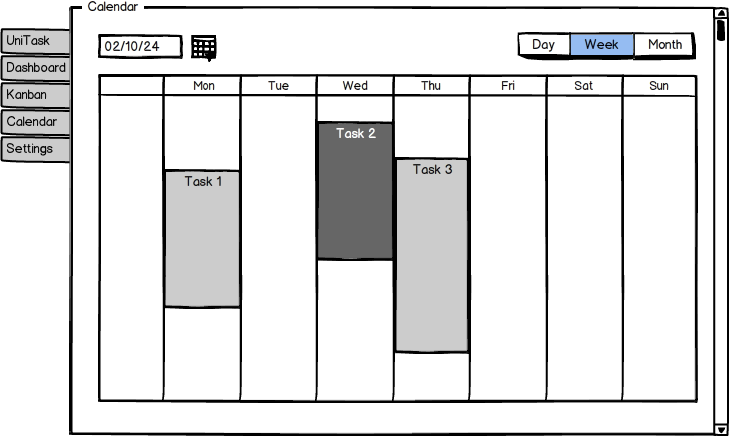
\includegraphics[width=0.65\textwidth]{mockups/Calendar}
            \caption{\centering Mockup Calendar σελίδας}
            \label{fig:unitaskMockupCalendar}
        \end{figure}

        \begin{figure}[h!] \noindent \centering
            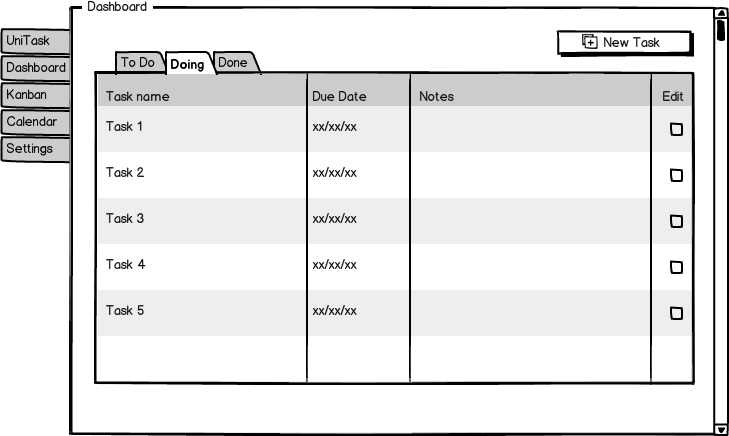
\includegraphics[width=0.65\textwidth]{mockups/Dashboard}
            \caption{\centering Mockup Dashboard σελίδας}
            \label{fig:unitaskMockupDashboard}
        \end{figure}

        \begin{figure}[h!] \noindent \centering
            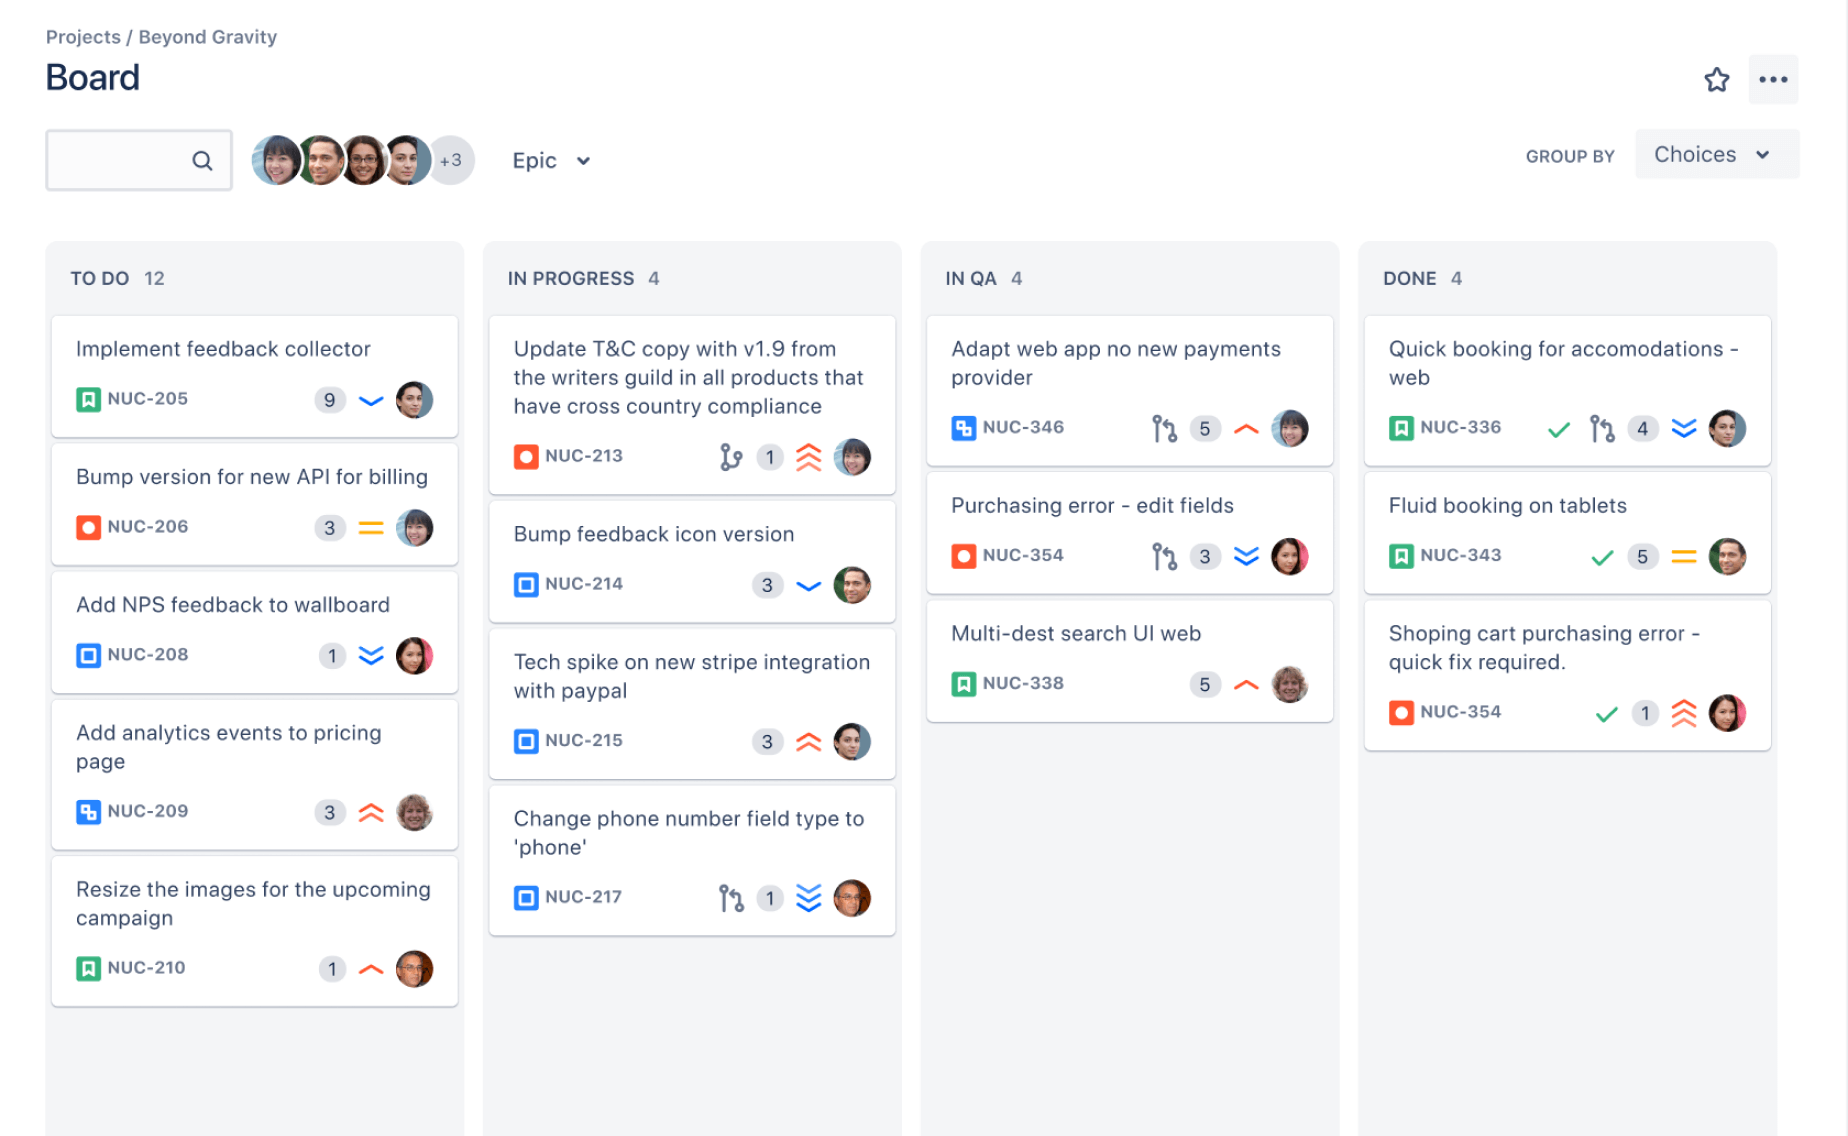
\includegraphics[width=0.65\textwidth]{mockups/Kanban}
            \caption{\centering Mockup Kanban σελίδας}
            \label{fig:unitaskMockupKanban}
        \end{figure}

    \pagebreak

    \section{Παρουσίαση της εφαρμογής}
        Κατά την εκτέλεση της εφαρμογής, είτε τοπικά είτε μέσω της απομακρυσμένης πρόσβασης στο cloud, στη διεύθυνση \texttt{https://unitask-sandbox.mxapps.io/}, εμφανίζεται αρχικά η \textbf{σελίδα σύνδεσης}, όπως φαίνεται στο σχήμα \ref{fig:unitask_Login}. Στη συγκεκριμένη σελίδα, οι χρήστες καλούνται να εισάγουν τα στοιχεία σύνδεσής τους για να αποκτήσουν πρόσβαση στις λειτουργίες της εφαρμογής.

        Το σύστημα αναγνωρίζει δύο επίπεδα πρόσβασης, ανάλογα με τα στοιχεία σύνδεσης που εισάγονται: δικαιώματα διαχειριστή (Administrator) και δικαιώματα χρήστη (User). Ο ρόλος του χρήστη (User) αντιστοιχεί σε φοιτητές που κάνουν χρήση της εφαρμογής, ενώ ο ρόλος του διαχειριστή παρέχει επιπλέον λειτουργίες διαχείρισης.

       \begin{figure}[h!] \noindent \centering
            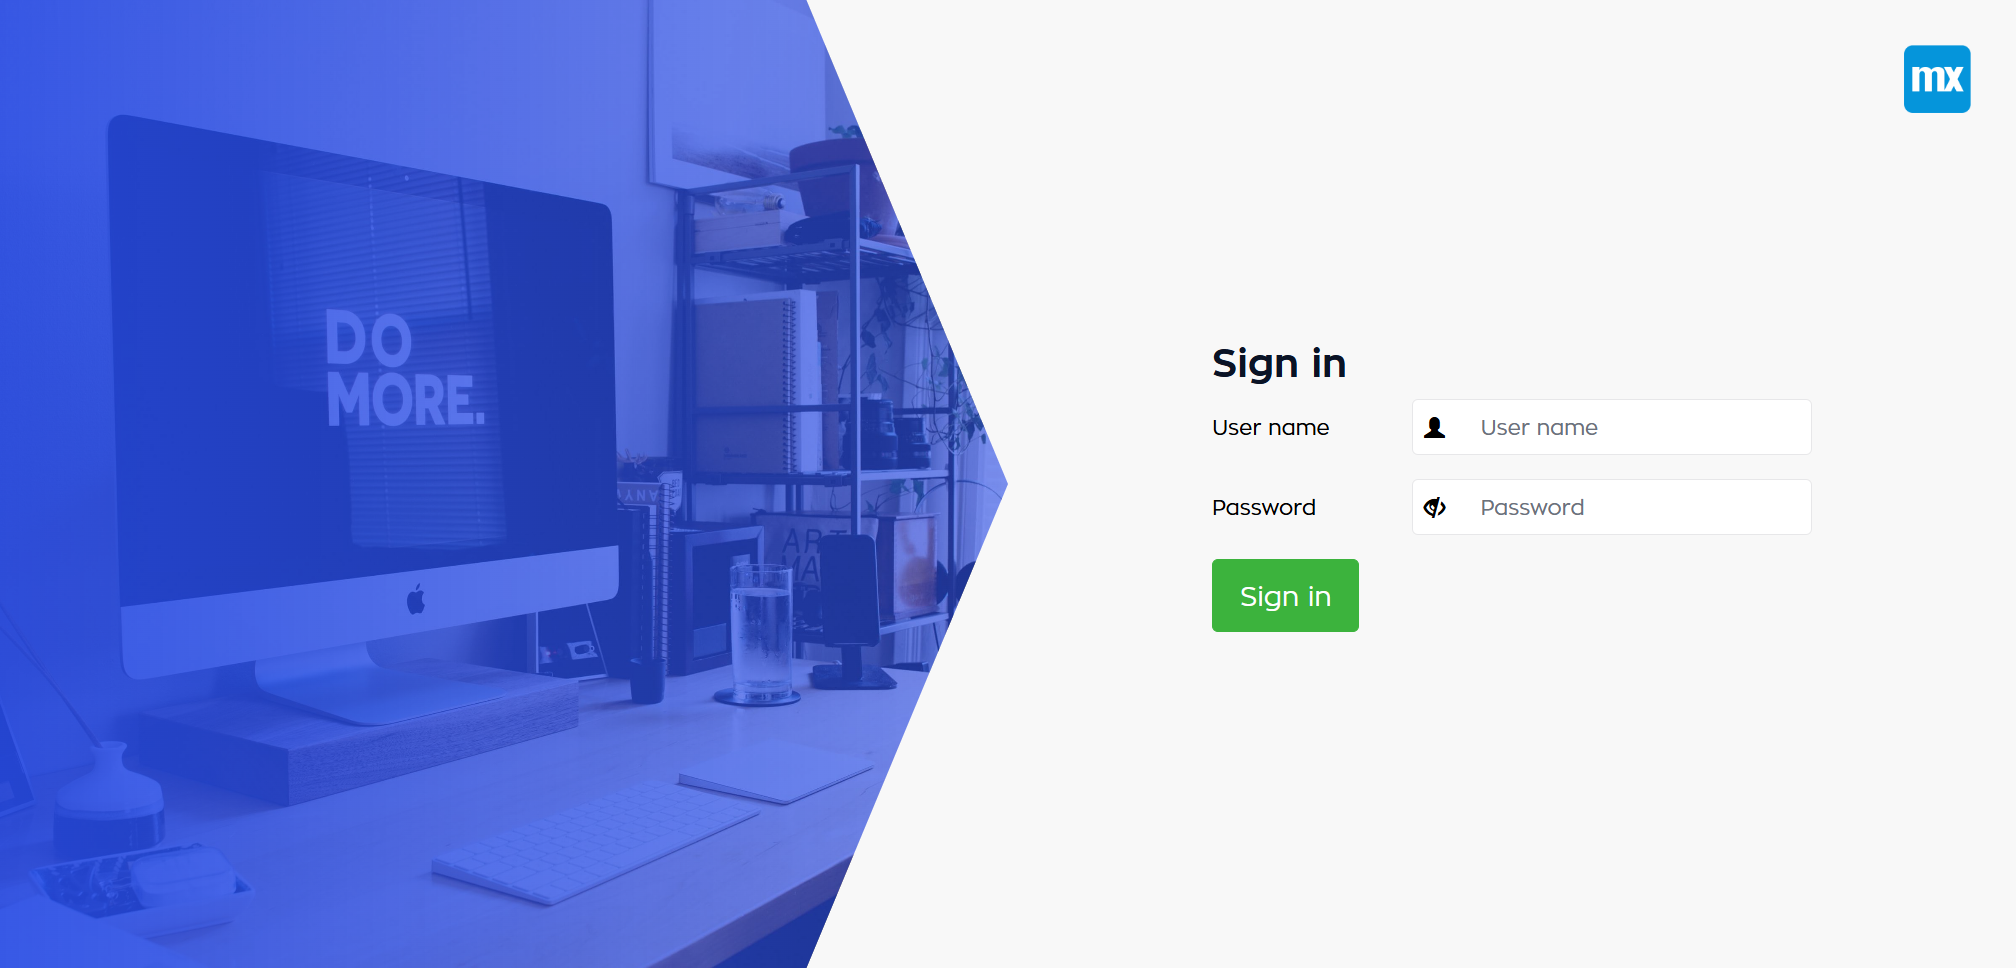
\includegraphics[width=\textwidth]{UniTask/Login}
            \caption{\centering Σελίδα σύνδεσης}
            \label{fig:unitask_Login}
        \end{figure}

        Αρχικά, πραγματοποιείται σύνδεση με τον λογαριασμό διαχειριστή (Administrator) προκειμένου να παρουσιαστούν οι λειτουργίες διαχείρισης χρηστών, συμπεριλαμβανομένης της δυνατότητας προσθήκης νέου χρήστη. Μετά την επιτυχή εισαγωγή των διαπιστευτηρίων του διαχειριστή, τα οποία έχουν οριστεί προκαταβολικά κατά την ανάπτυξη της εφαρμογής (βλ. ενότητα \ref{sec:unitask_mendix}), εμφανίζεται η \textbf{σελίδα διαχείρισης χρηστών}, όπως απεικονίζεται στο σχήμα \ref{fig:unitask_AccountOverview}. Η σελίδα αυτή παρέχει στους διαχειριστές μια ολοκληρωμένη επισκόπηση της λίστας χρηστών της εφαρμογής, καθώς και εργαλεία για τη διαχείρισή τους. Το layout της σελίδας αποτελείται από μια κάθετη μπάρα μενού η οποία περιλαμβάνει τις ίδιες δυνατότητες με τους απλούς χρήστες η οποίες θα αναλυθούν στη συνέχεια.

       \begin{figure}[h!] \noindent \centering
            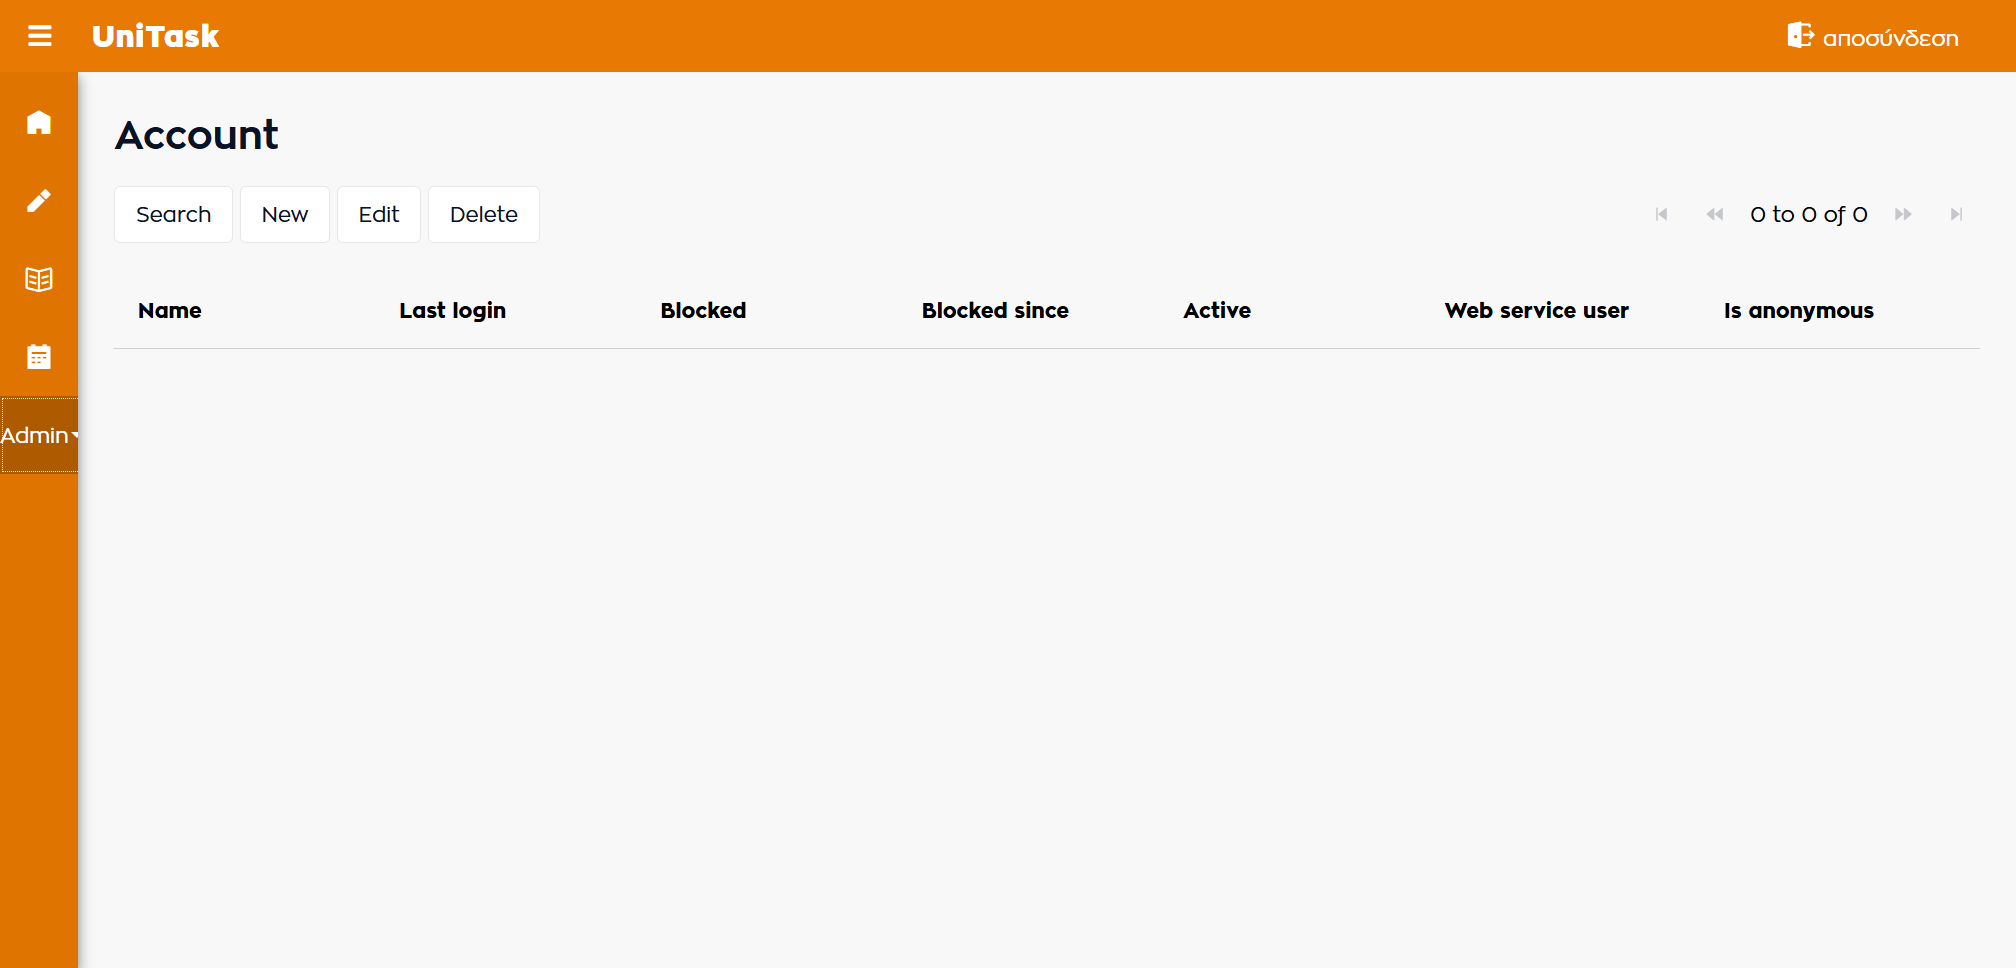
\includegraphics[trim={0 12cm 0 0}, clip, width=\textwidth]{UniTask/AccountOverview}
            \caption{\centering Σελίδα διαχείρισης χρηστών}
            \label{fig:unitask_AccountOverview}
        \end{figure}

        Πατώντας στο κουμπί {\Zona New}, εμφανίζεται η αναδυόμενη σελίδα του σχήματος \ref{fig:unitask_NewAccount} με μια \textbf{φόρμα για την προσθήκη νέου χρήστη}. Η φόρμα περιλαμβάνει πεδία για την εισαγωγή του ονόματος χρήστη ({\Zona Username}), του ρόλου του χρήστη ({\Zona User role}) όπου επιλέγεται αν πρόκειται για προσθήκη διαχειριστή ή χρήστη, του κωδικού πρόσβασης ({\Zona New password} και {\Zona Confirm password}). Λόγω του ότι ο χρήστης User έχει κληρονομήσει γνωρίσματα από την κλάση \texttt{System.User} του Mendix, έχουν προστεθεί πεδία όπως το {\Zona Blocked}, η οποία γίνεται αληθής μετά από κάποιες αποτυχημένες προσπάθειες σύνδεσης, το {\Zona Active} που γίνεται αληθές όταν ο χρήστης συνδεθεί, το {\Zona Time zone} όπου ορίζεται η ζώνη ώρας του χρήστη και το {\Zona Language} όπου ορίζεται η γλώσσα του χρήστη.

        \begin{figure}[h!] \noindent \centering
            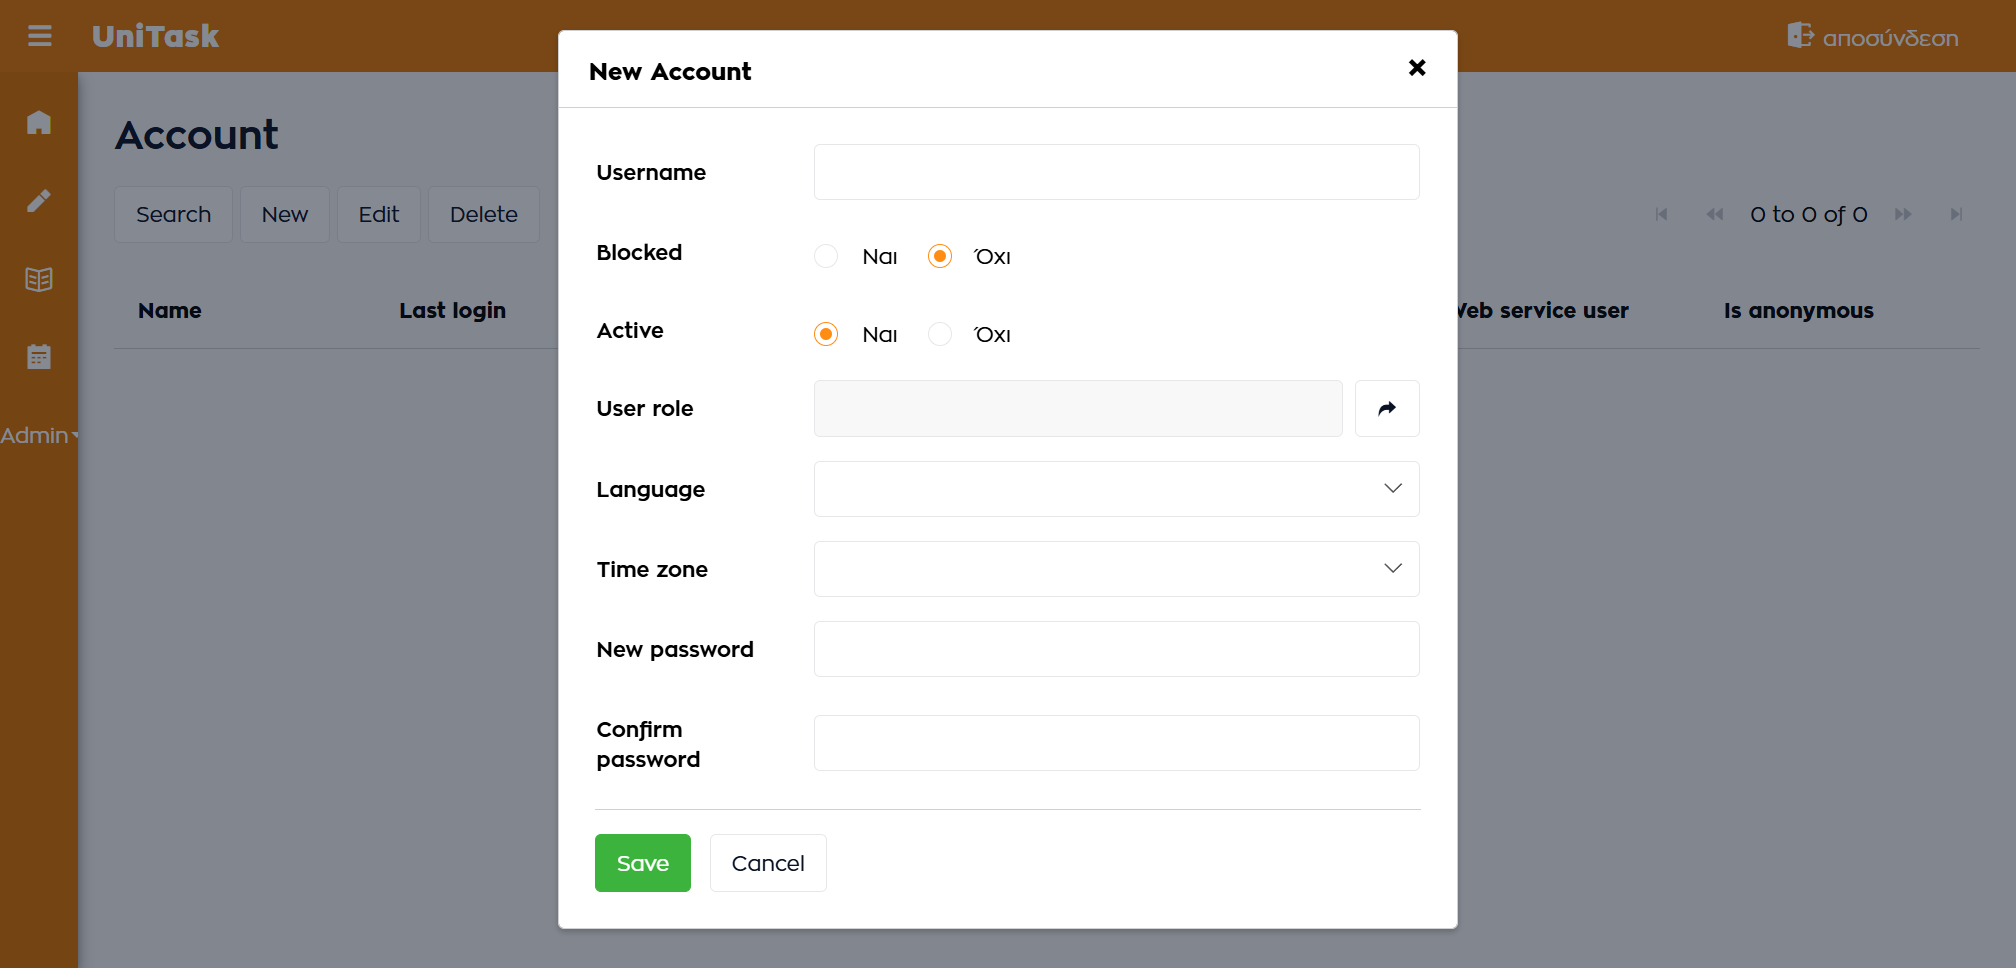
\includegraphics[width=\textwidth]{UniTask/NewAccount}
            \caption{\centering Φόρμα προσθήκης νέου χρήστη}
            \label{fig:unitask_NewAccount}
        \end{figure}

        Ένας νέος χρήστης δημιουργείται με το όνομα \texttt{Foithths}. Ο χρήστης προστίθεται στη λίστα χρηστών, όπως φαίνεται στο σχήμα \ref{fig:unitask_AccountOverview_WithStudent}. Πατώντας στο όνομά του, εμφανίζεται η σελίδα επεξεργασίας του χρήστη, όπως φαίνεται στο σχήμα \ref{fig:unitask_EditAccount}. Στη λίστα των χρηστών υπάρχει η δυνατότητα αναζήτησης χρηστών βάσει όλων των στοιχείων τους (σχήμα \ref{fig:unitask_SearchAccounts}), όπως επίσης και η δυνατότητα διαγραφής τους.

        \begin{figure}[h!] \noindent \centering
            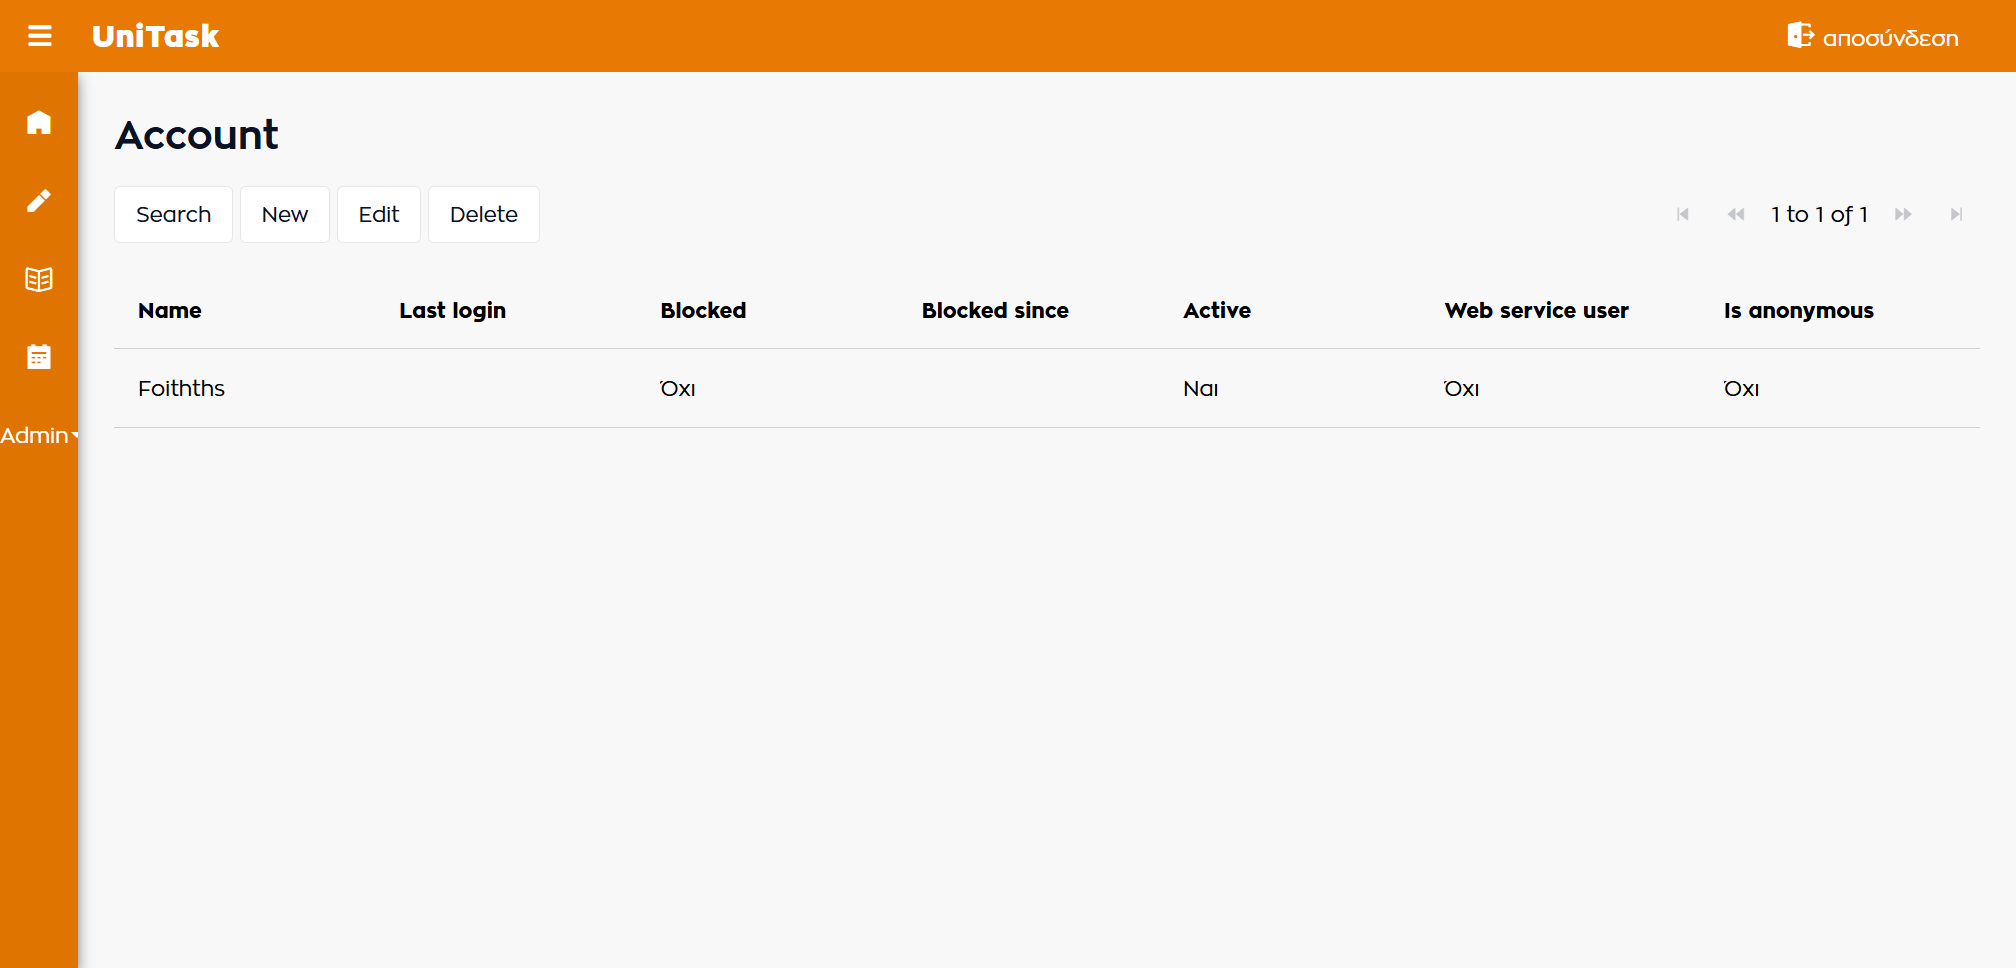
\includegraphics[trim={0 17cm 0 0}, clip, width=\textwidth]{UniTask/AccountOverview_WithStudent}
            \caption{\centering Λίστα χρηστών με τον χρήστη \texttt{Foithths}}
            \label{fig:unitask_AccountOverview_WithStudent}
        \end{figure}

        \begin{figure}[h!] \noindent \centering
            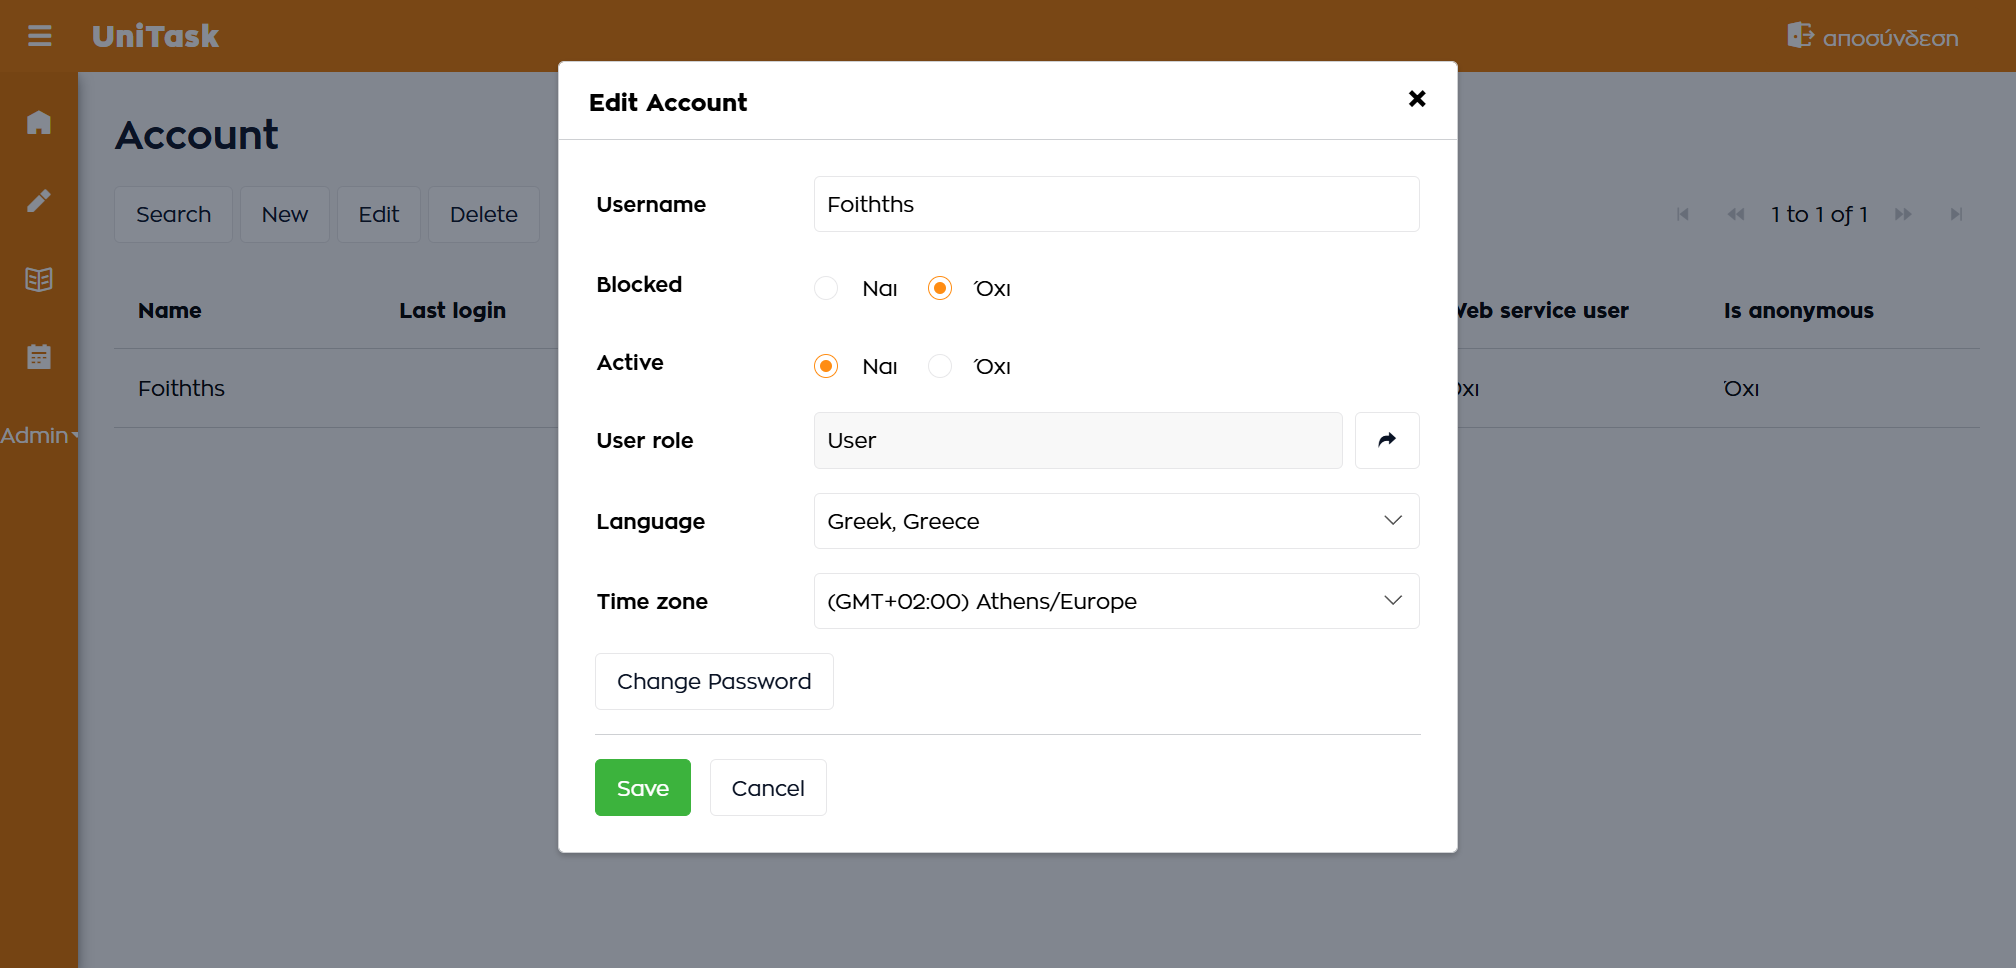
\includegraphics[trim={0 3cm 0 0}, clip, width=\textwidth]{UniTask/EditAccount}
            \caption{\centering Επεξεργασία στοιχείων χρήστη}
            \label{fig:unitask_EditAccount}
        \end{figure}

        \begin{figure}[h!] \noindent \centering
            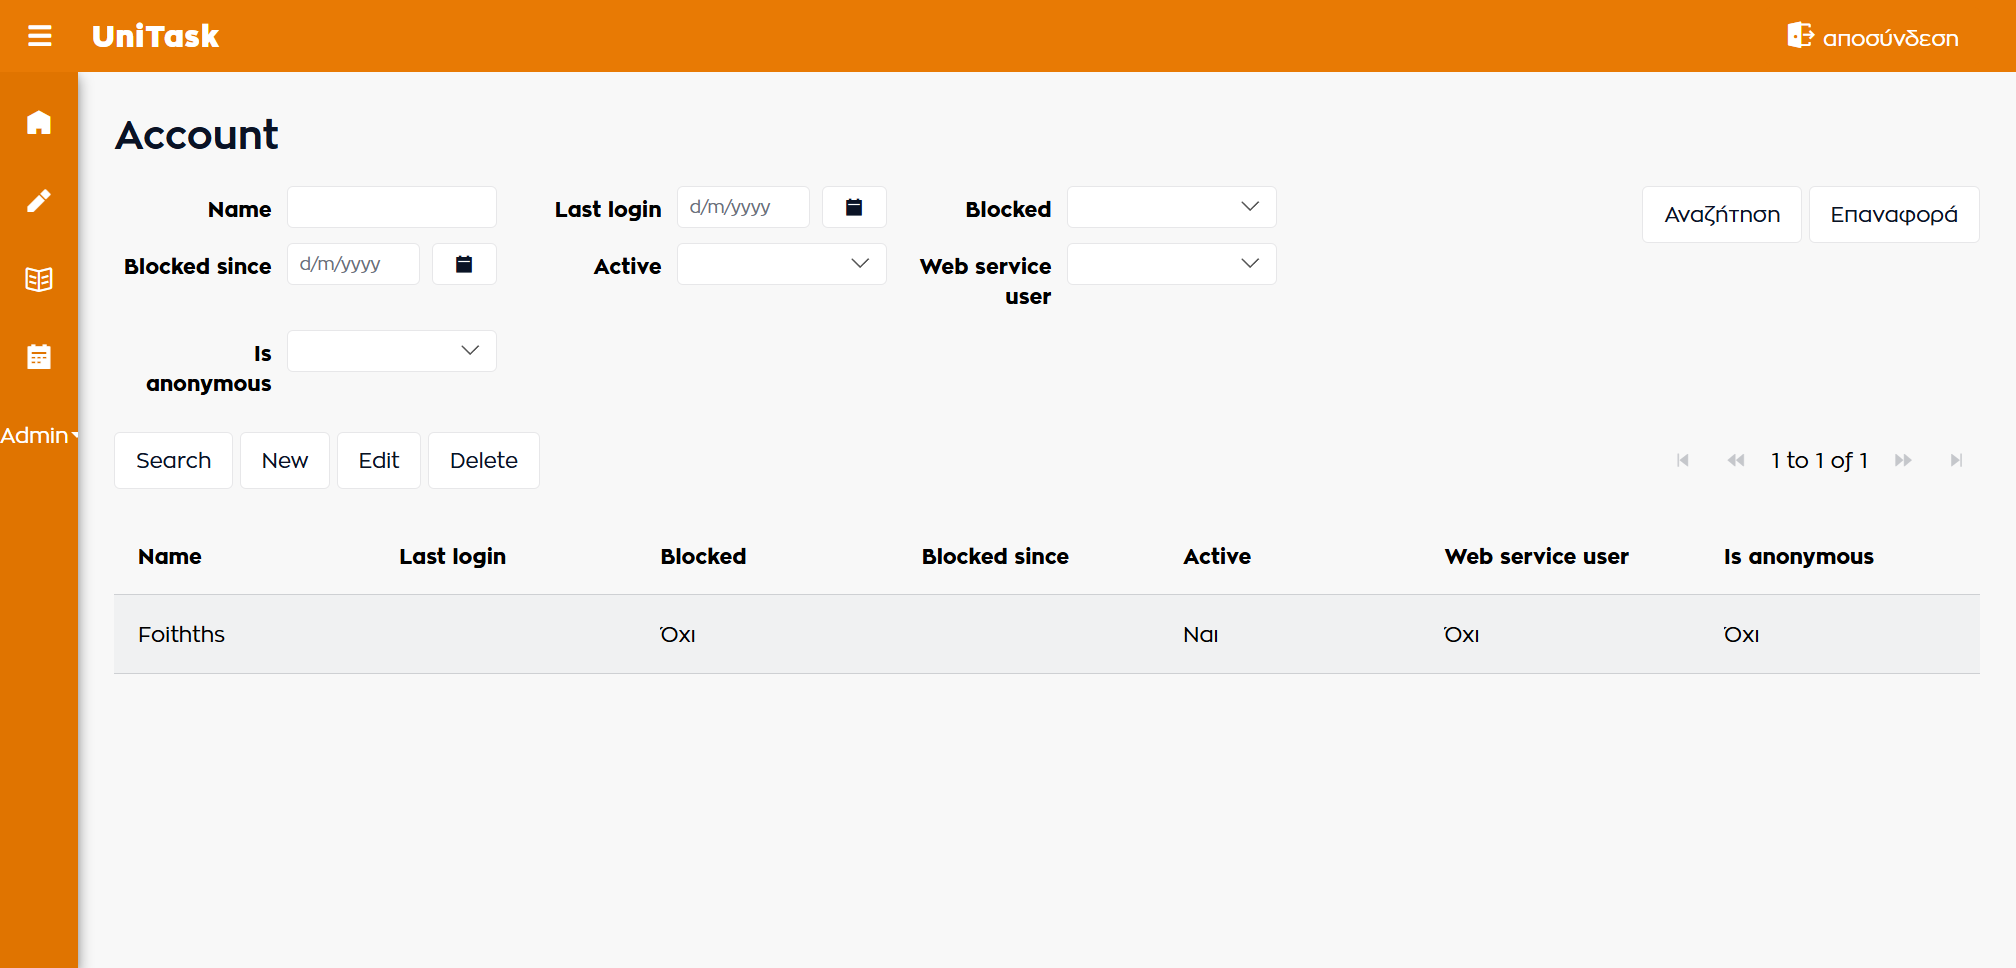
\includegraphics[trim={0 7cm 0 0}, clip, width=\textwidth]{UniTask/SearchAccounts}
            \caption{\centering Αναζήτηση χρήστη}
            \label{fig:unitask_SearchAccounts}
        \end{figure}

        Μετά την αποσύνδεση από τον λογαριασμό διαχειριστή και τη σύνδεση ως \texttt{Foithths}, εμφανίζεται η \textbf{αρχική σελίδα} της εφαρμογής (σχήμα \ref{fig:unitask_Home}). Η σελίδα περιλαμβάνει ένα κεντρικό call to action κουμπί ({\Zona όλες οι εργασίες}) το οποίο οδηγεί στο {\Zona dashboard}.

        \begin{figure}[h!] \noindent \centering
            
\includegraphics[width=\textwidth]{UniTask/Home}
            \caption{\centering Αρχική σελίδα εφαρμογής}
            \label{fig:unitask_Home}
        \end{figure}

        \begin{figure}[h!] \noindent \centering
            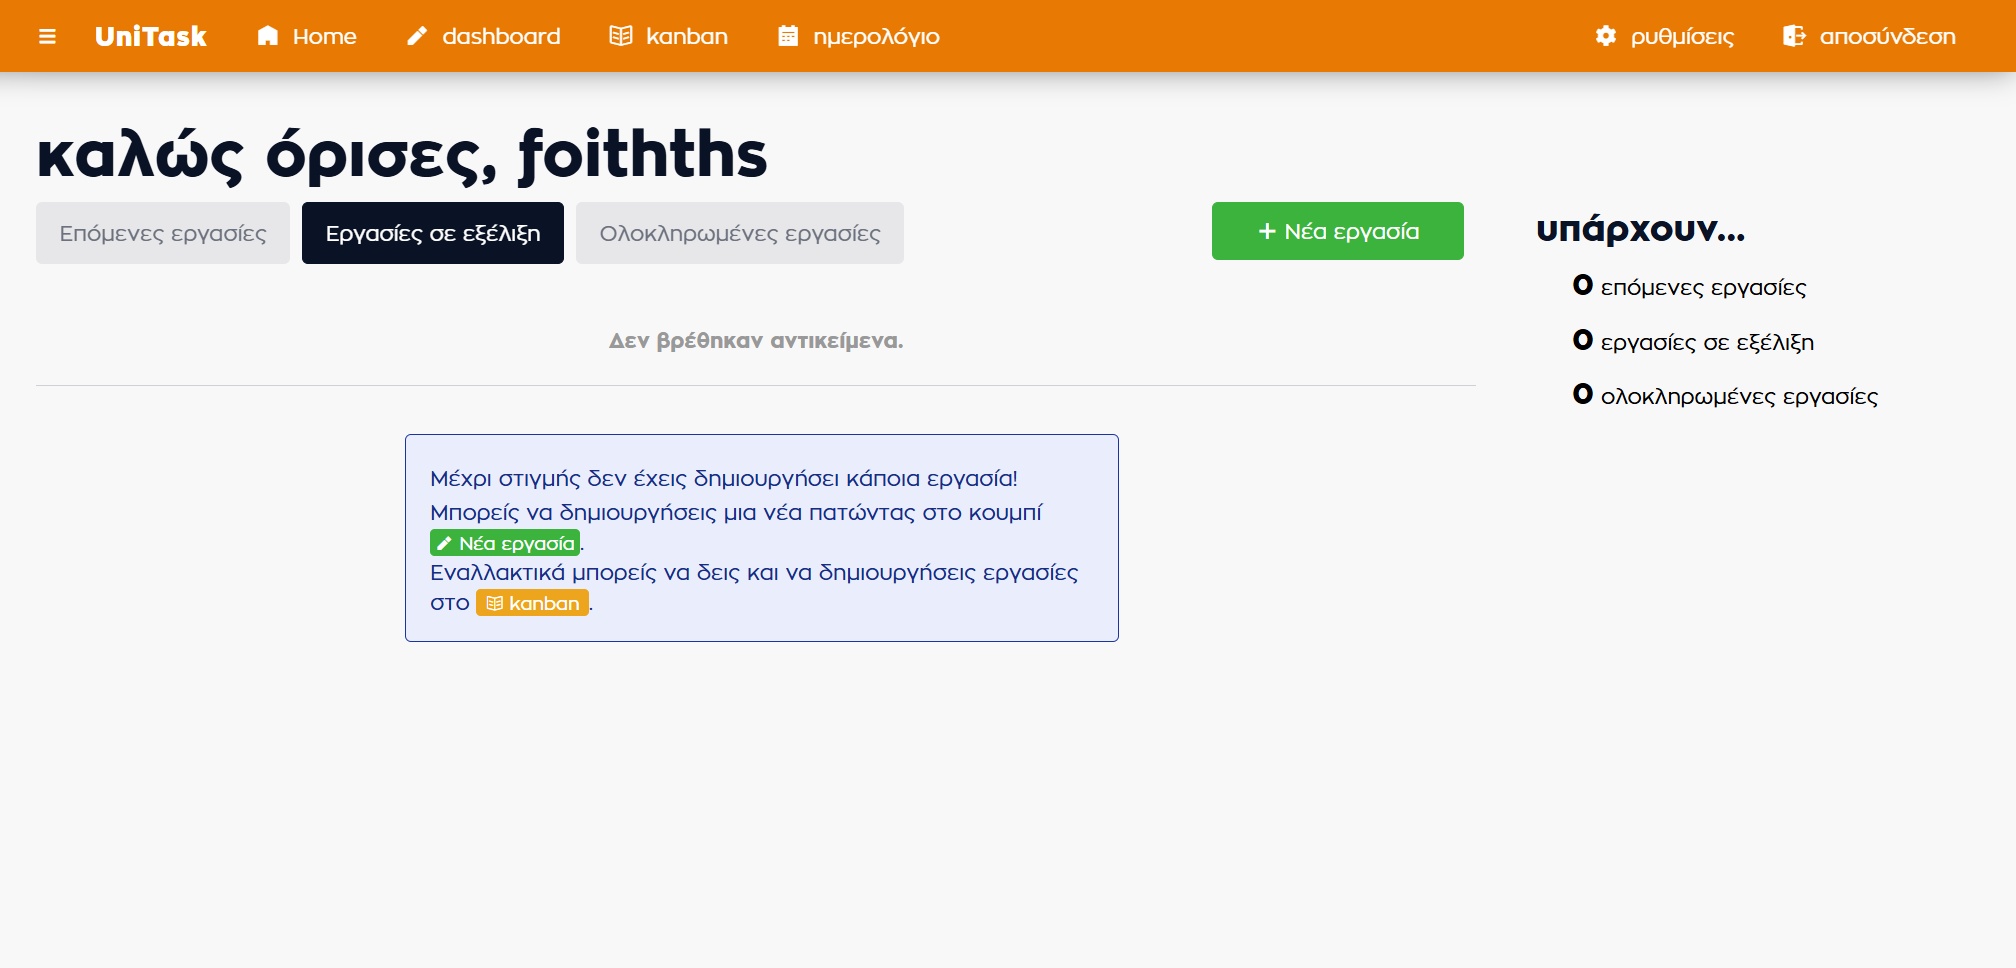
\includegraphics[width=\textwidth]{UniTask/TaskDashboard}
            \caption{\centering Dashboard εργασιών}
            \label{fig:unitask_TaskDashboard}
        \end{figure}

        Στο σχήμα \ref{fig:unitask_TaskDashboard} εμφανίζεται η σελίδα {\ZonaSB dashboard}. Πρόκειται για την κεντρική σελίδα προβολής, δημιουργίας και επεξεργασίας των εργασιών του χρήστη. Περιλαμβάνονται τρεις καρτέλες ({\Zona Επόμενες εργασίες}, {\Zona Εργασίες σε εξέλιξη}, {\Zona Ολοκληρωμένες εργασίες}). Οι επόμενες εργασίες αφορούν εργασίες που έχουν σκοπό να πραγματοποιηθούν στο άμεσο μέλλον αλλά όχι τη δεδομένη χρονική στιγμή, οι εργασίες σε εξέλιξη αφορούν εργασίες που βρίσκονται σε εξέλιξη και οι ολοκληρωμένες εργασίες αφορούν εργασίες που έχουν ολοκληρωθεί.

        Στη σελίδα επίσης περιλαμβάνεται ένα επεξηγηματικό παράθυρο που εμφανίζεται μόνο όταν ο χρήστης δεν έχει δημιουργήσει κάποια εργασία και του εξηγεί το τρόπο λειτουργίας της εφαρμογής. Στο {\Zona dashboard} επίσης περιλαμβάνονται μετρητές για το σύνολο των εργασιών που υπάρχουν ανά κατηγορία, όπως επίσης και ένα κεντρικό κουμπί δημιουργίας εργασιών ({\Zona Νέα εργασία}).

        \begin{figure}[h!] \noindent \centering
            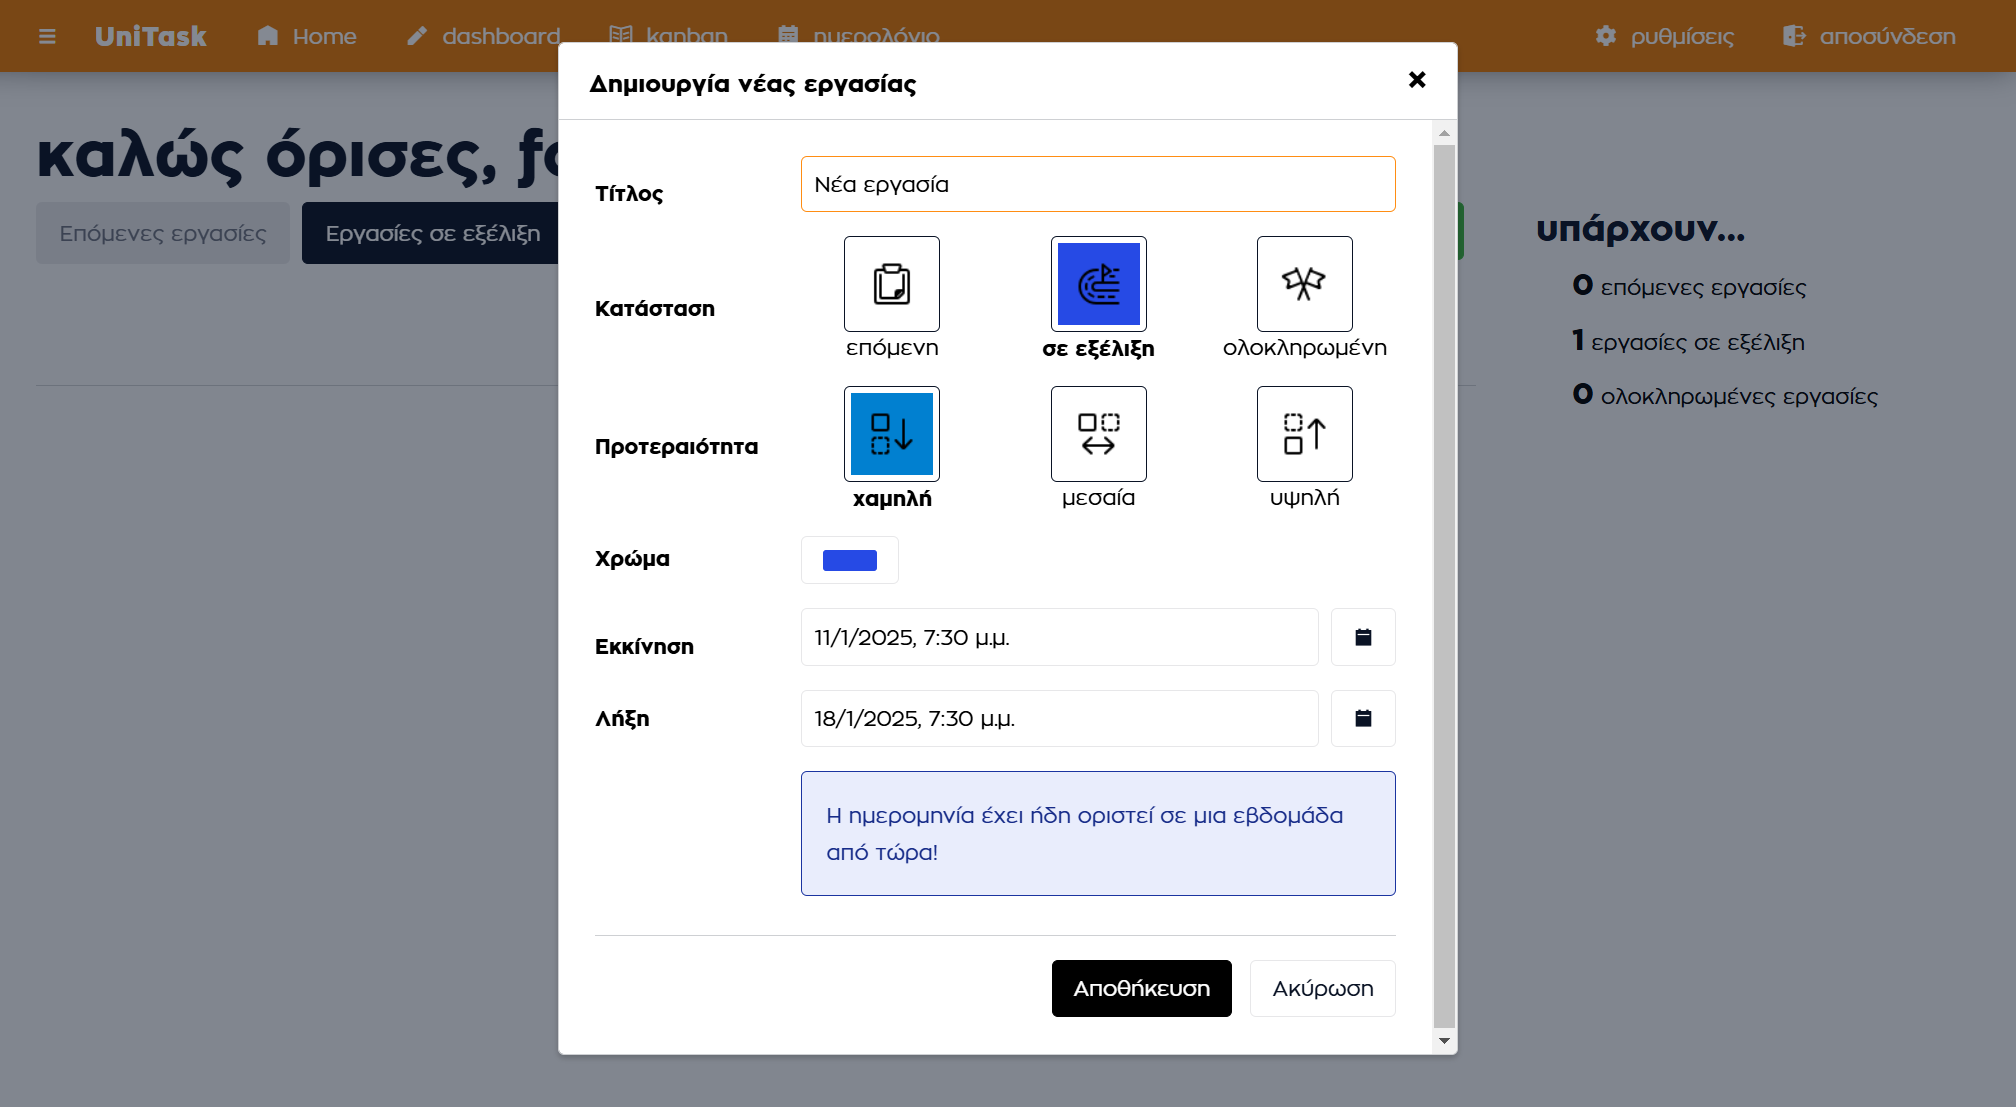
\includegraphics[width=\textwidth]{UniTask/NewTask_Default}
            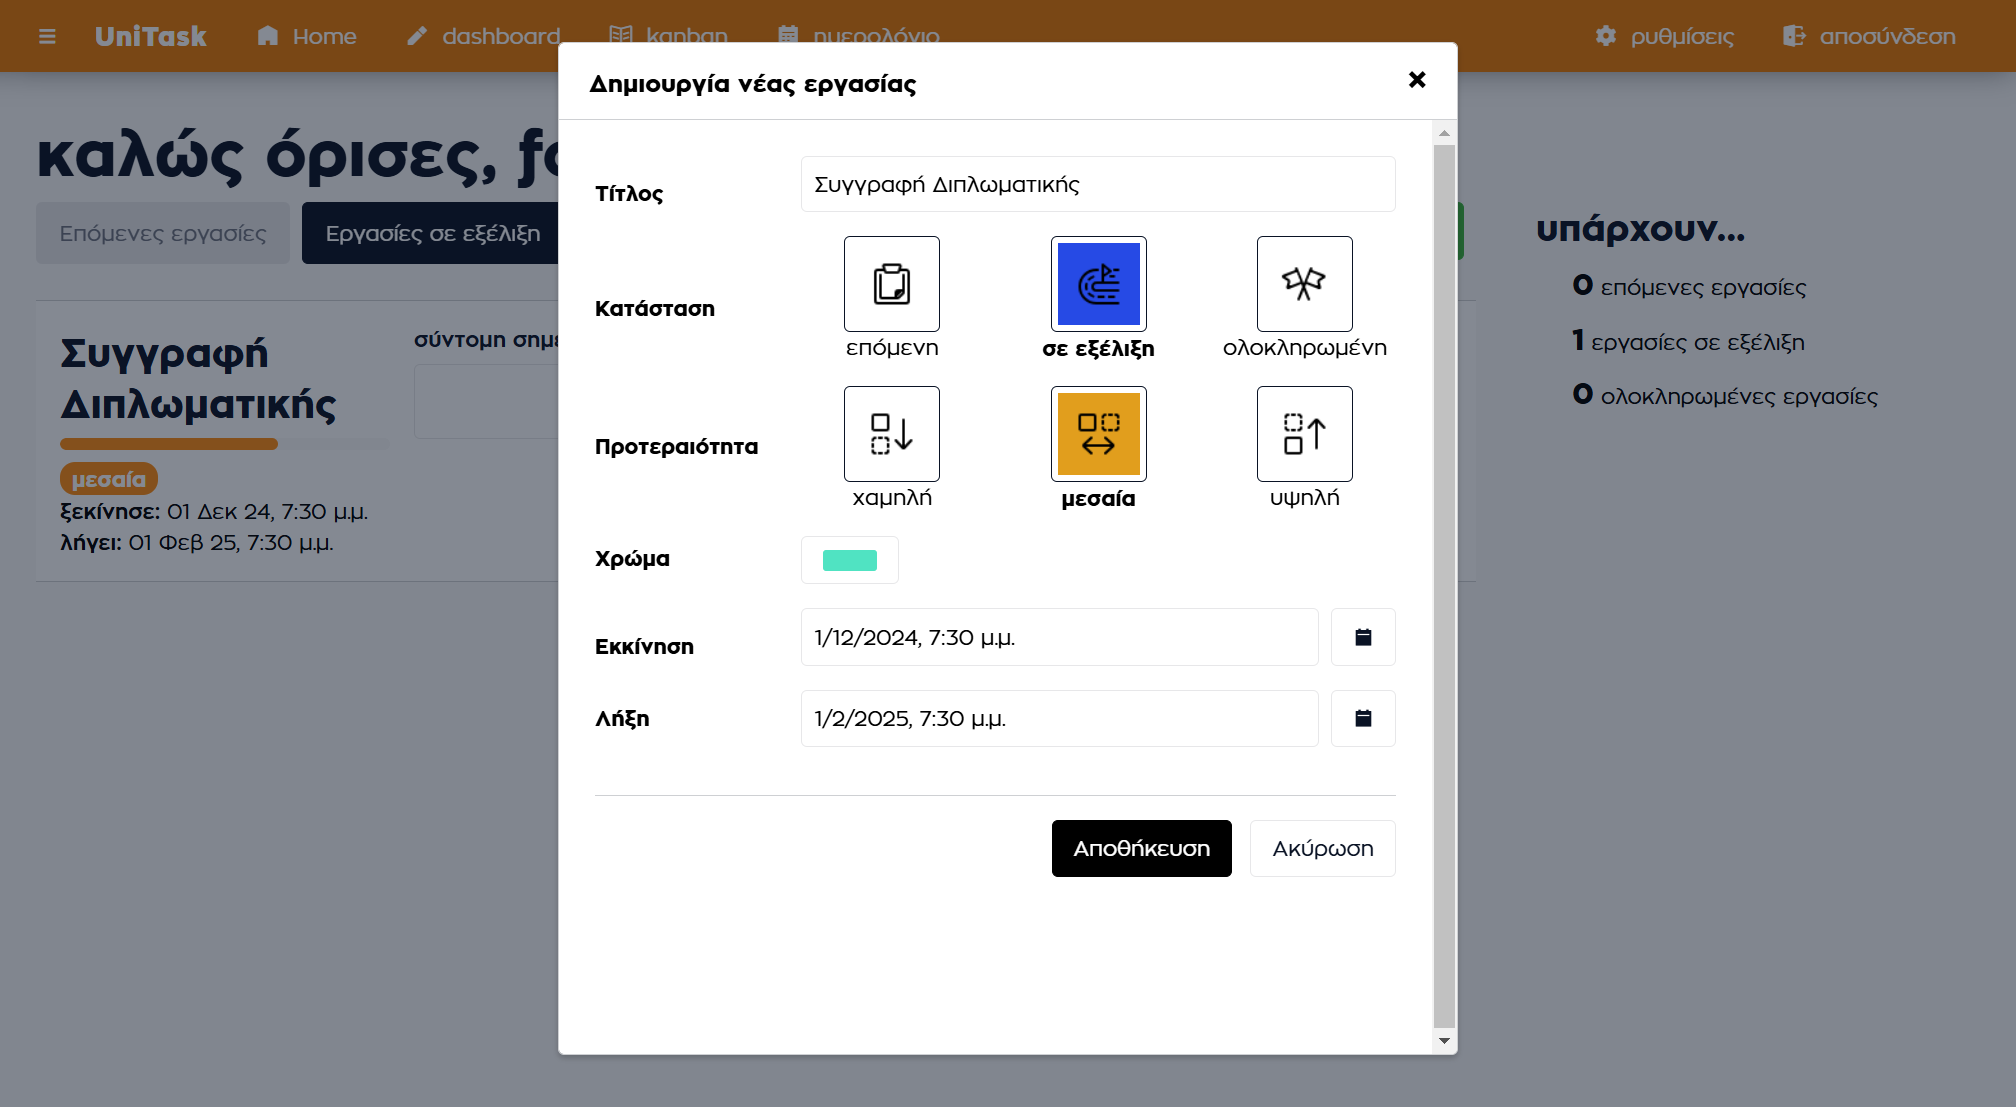
\includegraphics[width=\textwidth]{UniTask/NewTask_Finished}
            \caption{\centering Δημιουργία νέας εργασίας}
            \label{fig:unitask_NewTask}
        \end{figure}

        Πατώντας το, εμφανίζεται ένα αναδυόμενο παράθυρο (σχήμα \ref{fig:unitask_NewTask}.1) με μια φόρμα για τη δημιουργία μιας νέας εργασίας. Η φόρμα αυτή περιλαμβάνει πεδία για την εισαγωγή του τίτλου της εργασίας ({\Zona Τίτλος}), της ημερομηνίας έναρξης ({\Zona Εκκίνηση}) και λήξης ({\Zona Λήξη}), της κατάστασης της εργασίας ({\Zona Κατάσταση}), της προτεραιότητας της εργασίας ({\Zona Προτεραιότητα}) όπως επίσης και του χρώματος της εργασίας ({\Zona Χρώμα}), όπως θα αποτυπωθεί μετέπειτα στο ημερολόγιο. Στο αναδυόμενο παράθυρο ορίζεται προεπιλεγμένα ως ημερομηνία λήξης της εργασίας μια εβδομάδα μετέπειτα από την ημερομηνία δημιουργίας της, ενώ η κατάσταση της εργασίας έχει προκαθοριστεί (γίνεται να τροποποιηθεί φυσικά) ανάλογα με το ποια καρτέλα ήταν ανοιχτή στο dashboard. Αφού επεξεργαστούμε το παράθυρο όπως επιθυμούμε (σχήμα \ref{fig:unitask_NewTask}.2), πατάμε αποθήκευση για την αποθήκευση της εργασίας.

        Σημειώνεται ότι οι επιλογές για την κατάσταση και την προτεραιότητα της εργασίας είναι χρωματικά κωδικοποιημένες (color-coded) και συνοδεύονται από γραφικά σύμβολα, όπως φαίνεται στο σχήμα \ref{fig:unitask_NewTask_AllOptions} με σκοπό να διευκολύνει τον χρήστη για την άμεση αναγνώριση τους.

        \begin{figure}[h!] \noindent \centering
            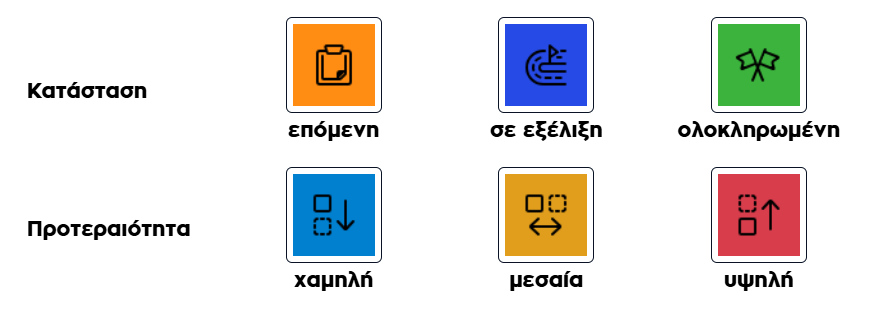
\includegraphics[width=0.7\textwidth]{UniTask/NewTask_AllOptions}
            \caption{\centering Επιλογές κατάστασης και προτεραιότητας εργασίας}
            \label{fig:unitask_NewTask_AllOptions}
        \end{figure}

        \begin{figure}[h!] \noindent \centering
            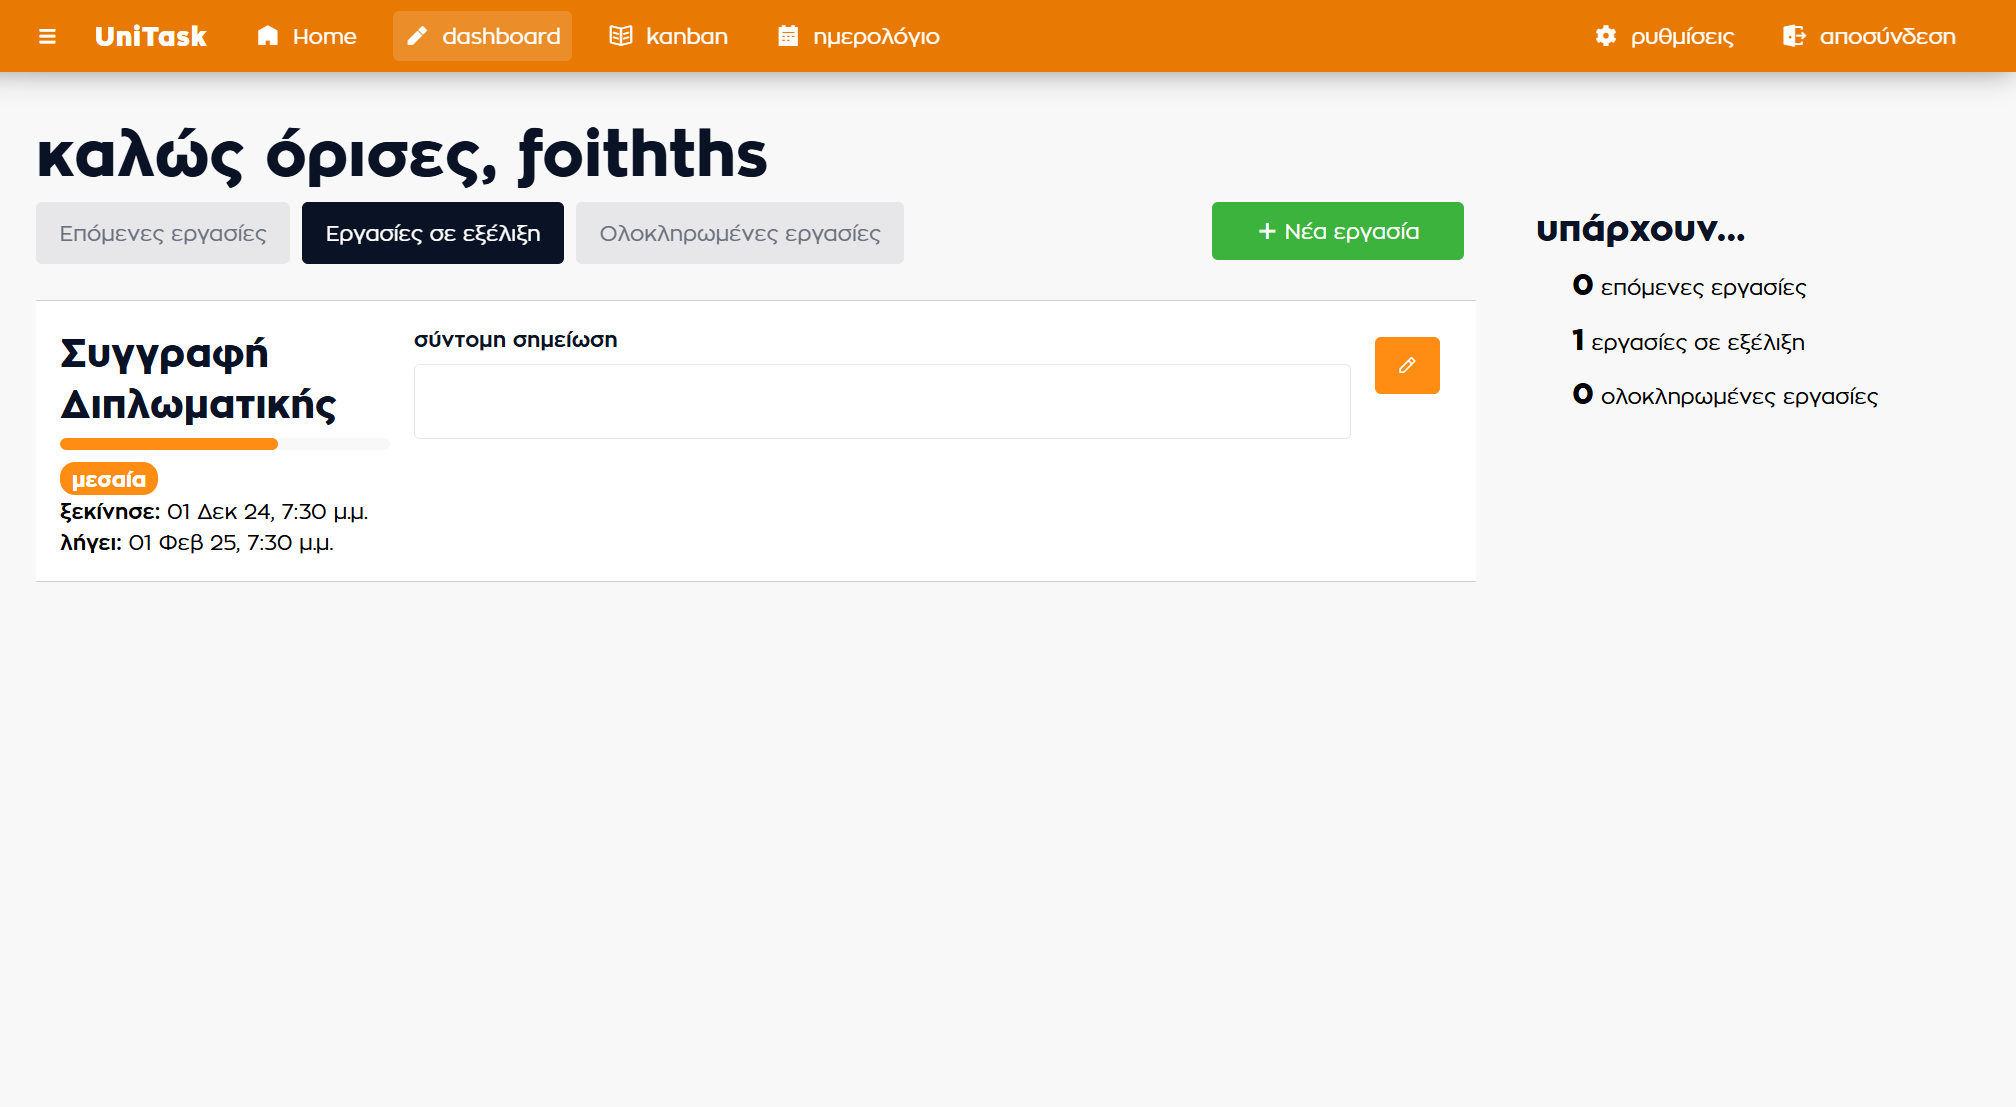
\includegraphics[trim={0 10cm 0 0}, clip, width=\textwidth]{UniTask/TaskDashboard_WithTask}
            \caption{\centering Dashboard με δημιουργημένη εργασία}
            \label{fig:unitask_TaskDashboard_WithTask}
        \end{figure}

        Στη σελίδα πλέον είναι δημιουργημένη η κάρτα με την πρώτη μας εργασία (σχήμα \ref{fig:unitask_TaskDashboard_WithTask}). Το πλαίσιο {\Zona σύντομη σημείωση} επιτρέπει την εισαγωγή μιας συνοπτικής περιγραφής της εργασίας, στα αριστερά εμφανίζεται ο τίτλος της εργασίας, μια μπάρα προόδου (progress bar) η οποία δυναμικά αυξάνεται όσο πλησιάζουμε στη λήξη της εργασίας, όπως επίσης η προτεραιότητα της εργασίας και οι ημερομηνίες και ώρες εκκίνησης και λήξης της εργασίας, ενώ στο δεξί μέρος της κάρτας εμφανίζονται το εικονίδιο για την επεξεργασία της εργασίας.

        Η ταξινόμηση των εργασιών στο dashboard βασίζεται στην προτεραιότητα και στον χρόνο λήξης τους. Έτσι μια εργασία με υψηλή προτεραιότητα θα εμφανίζεται ψηλότερα από μια εργασία με χαμηλή προτεραιότητα που δε λήγει σύντομα.

        \begin{figure}[h!] \noindent \centering
            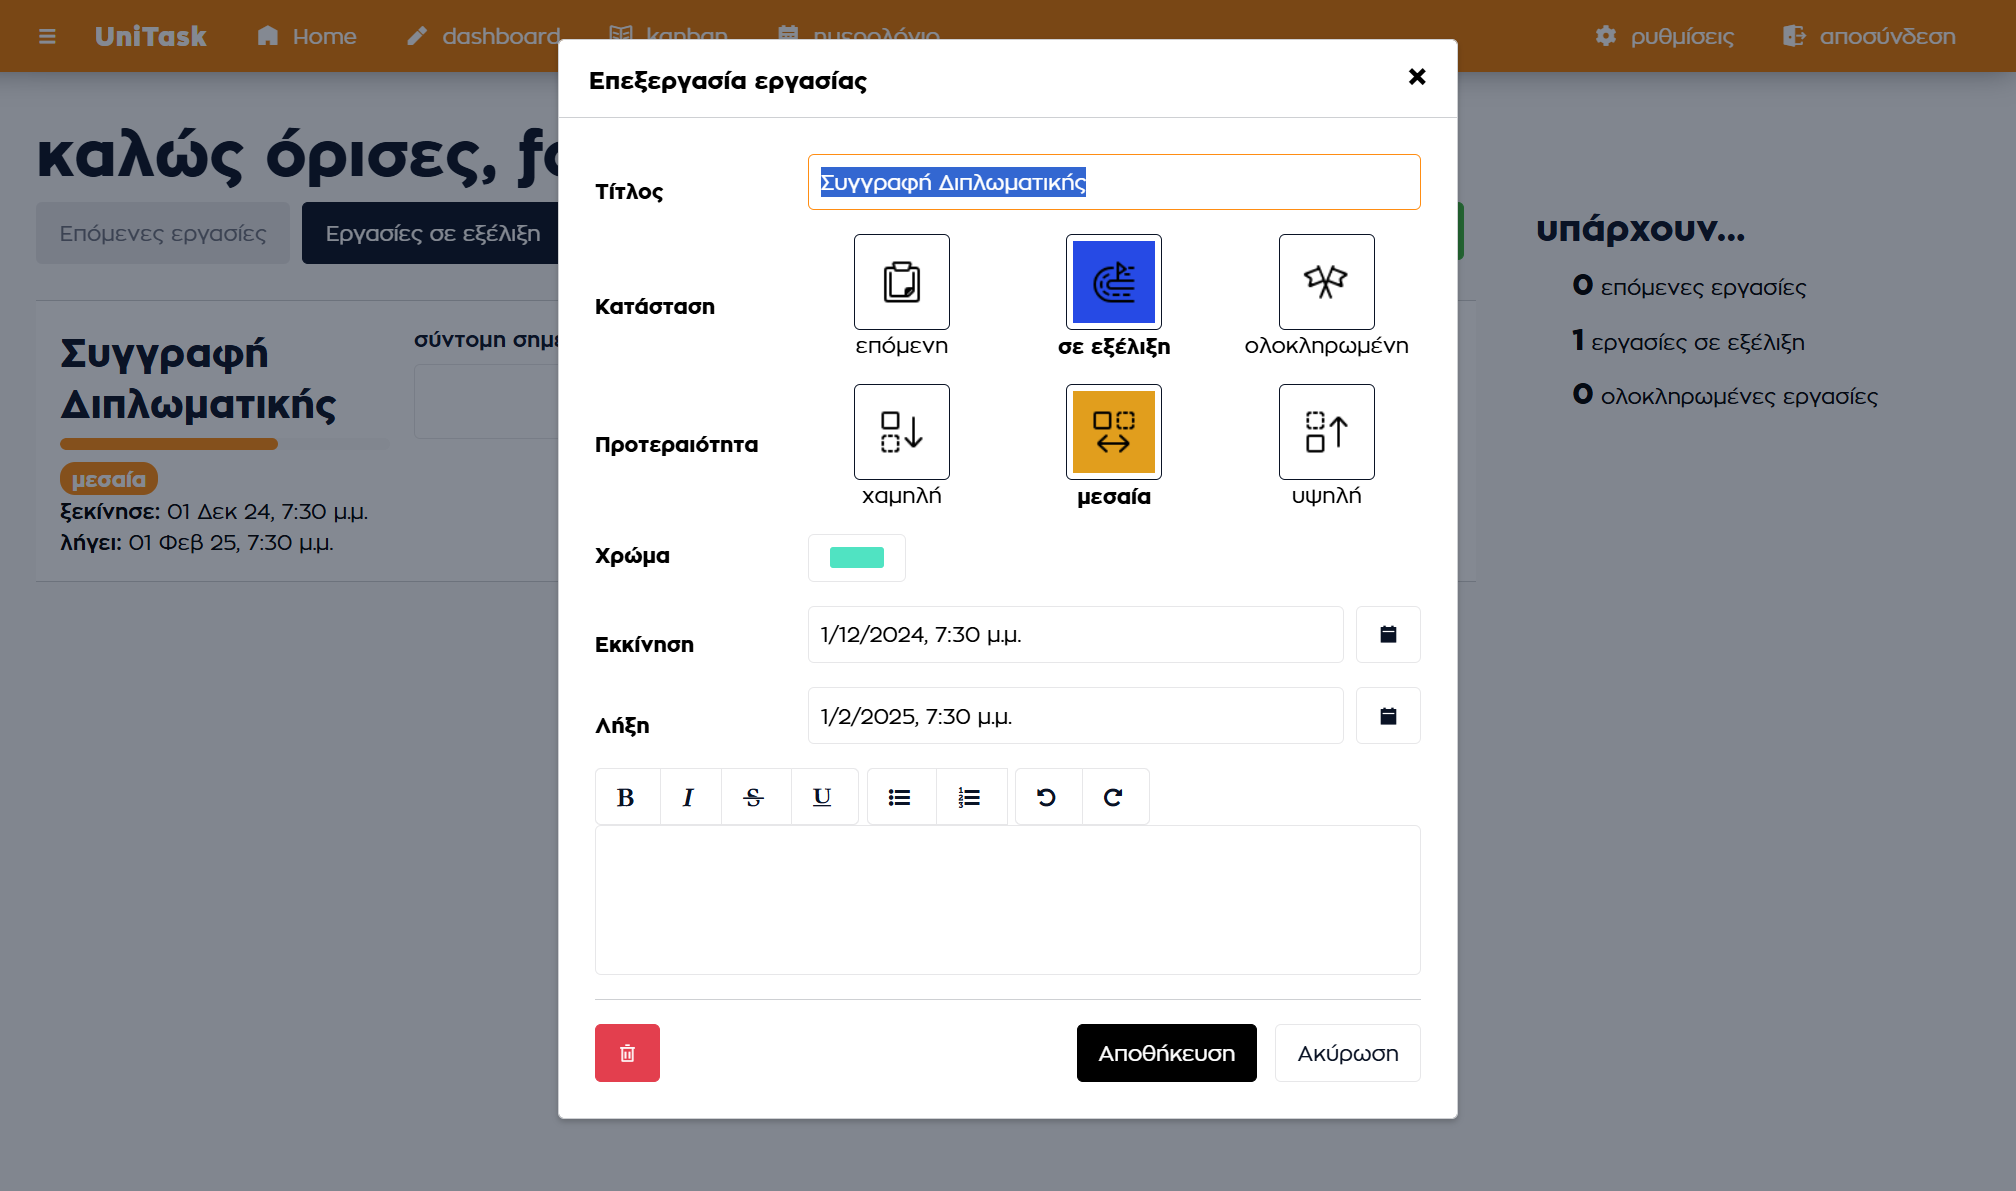
\includegraphics[width=\textwidth]{UniTask/EditTask}
            \caption{\centering Επεξεργασία εργασίας}
            \label{fig:unitask_EditTask}
        \end{figure}

        Με την επιλογή του εικονιδίου επεξεργασίας, εμφανίζεται το αναδυόμενο παράθυρο (σχήμα \ref{fig:unitask_EditTask}), το οποίο επιτρέπει την τροποποίηση των στοιχείων της εργασίας, συμπεριλαμβανομένου του πλαισίου {\Zona σύντομη σημείωση}. Το ίδιο παράθυρο περιλαμβάνει και το κουμπί διαγραφής της εργασίας.

        Για την καλύτερη διευκόλυνση του χρήστη, την τελευταία εβδομάδα πριν λήξη της προθεσμίας εμφανίζεται ενημερωτικό κείμενο στην κάρτα (σχήμα \ref{fig:unitask_cardInfo}.1), ενώ όταν η εργασία έχει λήξει, εμφανίζεται call-to-action κουμπί που μπορεί να μετακινήσει αυτήν την εργασία στις ολοκληρωμένες εργασίες (σχήμα \ref{fig:unitask_cardInfo}.2).

        \begin{figure}[h!] \noindent \centering
            
\includegraphics[width=\textwidth]{UniTask/προθεσμία λήγει}
            
\includegraphics[width=\textwidth]{UniTask/προθεσμία έληξε}
            \caption{\centering Ενημερωτικό κείμενο κάρτας εργασίας}
            \label{fig:unitask_cardInfo}
        \end{figure}

        Επίσης, κατά την αλλαγή κατηγορίας της εργασίας σε ολοκληρωμένη, εμφανίζονται κομφετί ως ένα σύστημα ανταμοιβής για τον χρήστη (σχήμα \ref{fig:unitask_confetti}).

        \begin{figure}[h!] \noindent \centering
            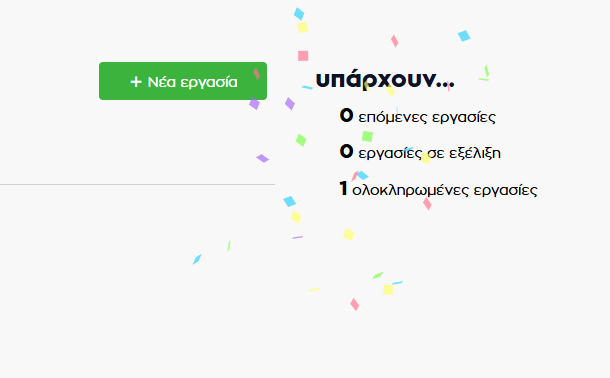
\includegraphics[width=0.7\textwidth]{UniTask/κομφετί}
            \caption{\centering Επιβράβευση όταν ολοκληρωθεί μια εργασία}
            \label{fig:unitask_confetti}
        \end{figure}

        \begin{figure}[h!] \noindent \centering
            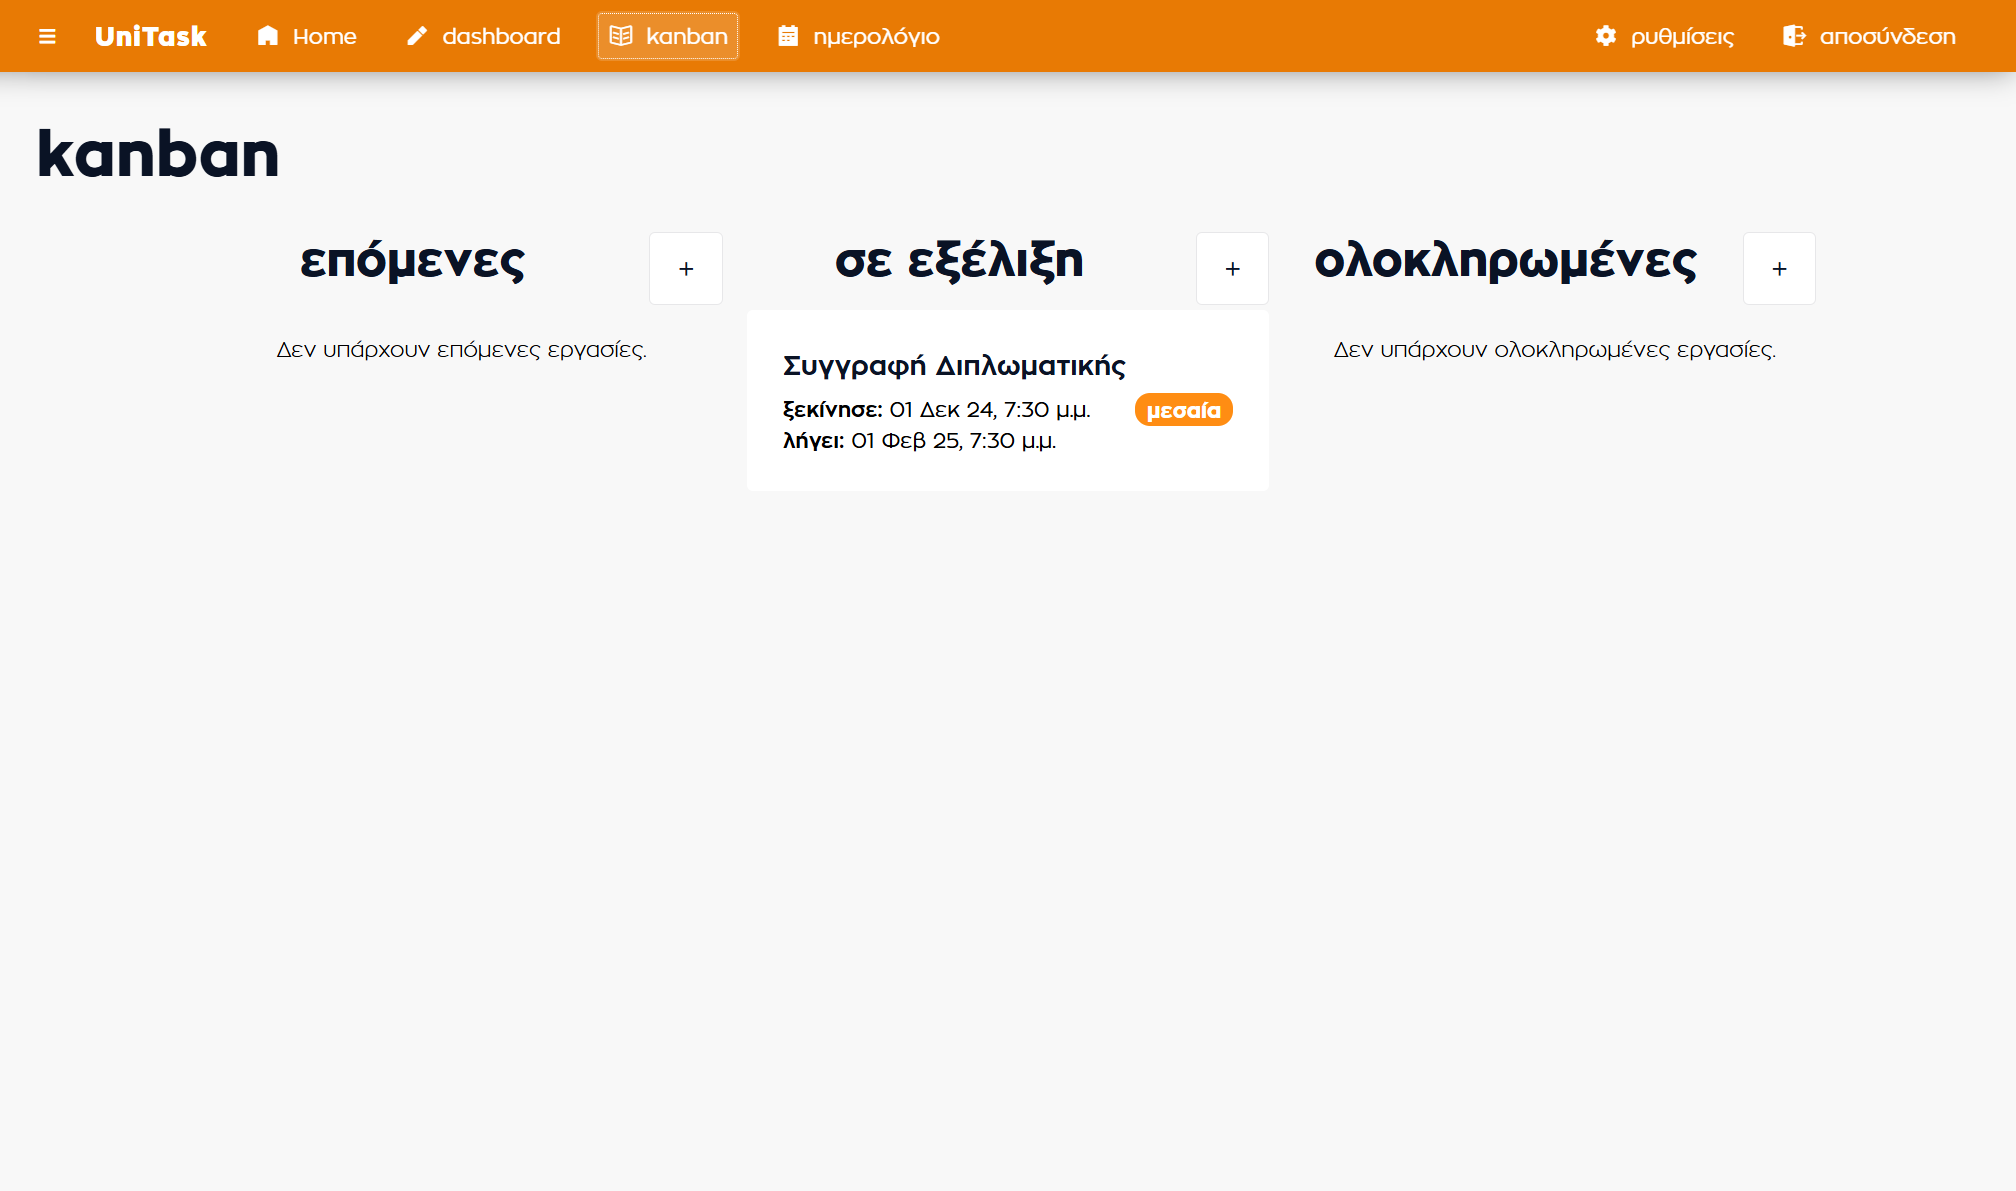
\includegraphics[trim={0 10cm 0 0}, clip, width=\textwidth]{UniTask/Kanban_WithTask}
            \caption{\centering Σελίδα Kanban}
            \label{fig:unitask_Kanban_WithTask}
        \end{figure}

        Η σελίδα {\ZonaSB Kanban} του σχήματος \ref{fig:unitask_Kanban_WithTask} εμφανίζει μια διαφορετική παρουσίαση στις εργασίες με τον τρόπο που έχει εξηγηθεί στην ενότητα \ref{subsec:Kanban}. Στον πίνακα Kanban οι εργασίες χωρίζονται σε τρεις κατηγορίες: τις εργασίες που έχουν ολοκληρωθεί, τις εργασίες που βρίσκονται σε εξέλιξη και τις εργασίες που έχουν σκοπό να πραγματοποιηθούν στο μέλλον. Κάθε στήλη περιλαμβάνει ένα κουμπί δημιουργίας νέας εργασίας που αυτόματα καθορίζει και την κατηγορία της.

        Οι εργασίες απεικονίζονται ως κάρτες που περιλαμβάνουν τον τίτλο, την προτεραιότητα, καθώς και την ημερομηνία έναρξης και λήξης τους, ενώ πατώντας πάνω στην κάρτα μιας εργασίας, εμφανίζεται το αναδυόμενο παράθυρο επεξεργασίας της εργασίας του σχήματος \ref{fig:unitask_EditTask}.

        Στη σελίδα {\ZonaSB ημερολόγιο} (σχήμα \ref{fig:unitask_Calendar_WithTask}) εμφανίζεται ένα ημερολόγιο με τις εργασίες του χρήστη. Οι εργασίες εμφανίζονται στο ημερολόγιο με το χρώμα που έχει οριστεί στην επιλογή του χρήστη κατά τη δημιουργία της εργασίας, υπάρχουν προβολές ανά ημέρα, εβδομάδα ή μήνα ενώ εμφανίζεται και ένα σύντομο παράρτημα στα δεξιά με τη λίστα των εργασιών.

        \begin{figure}[h!] \noindent \centering
            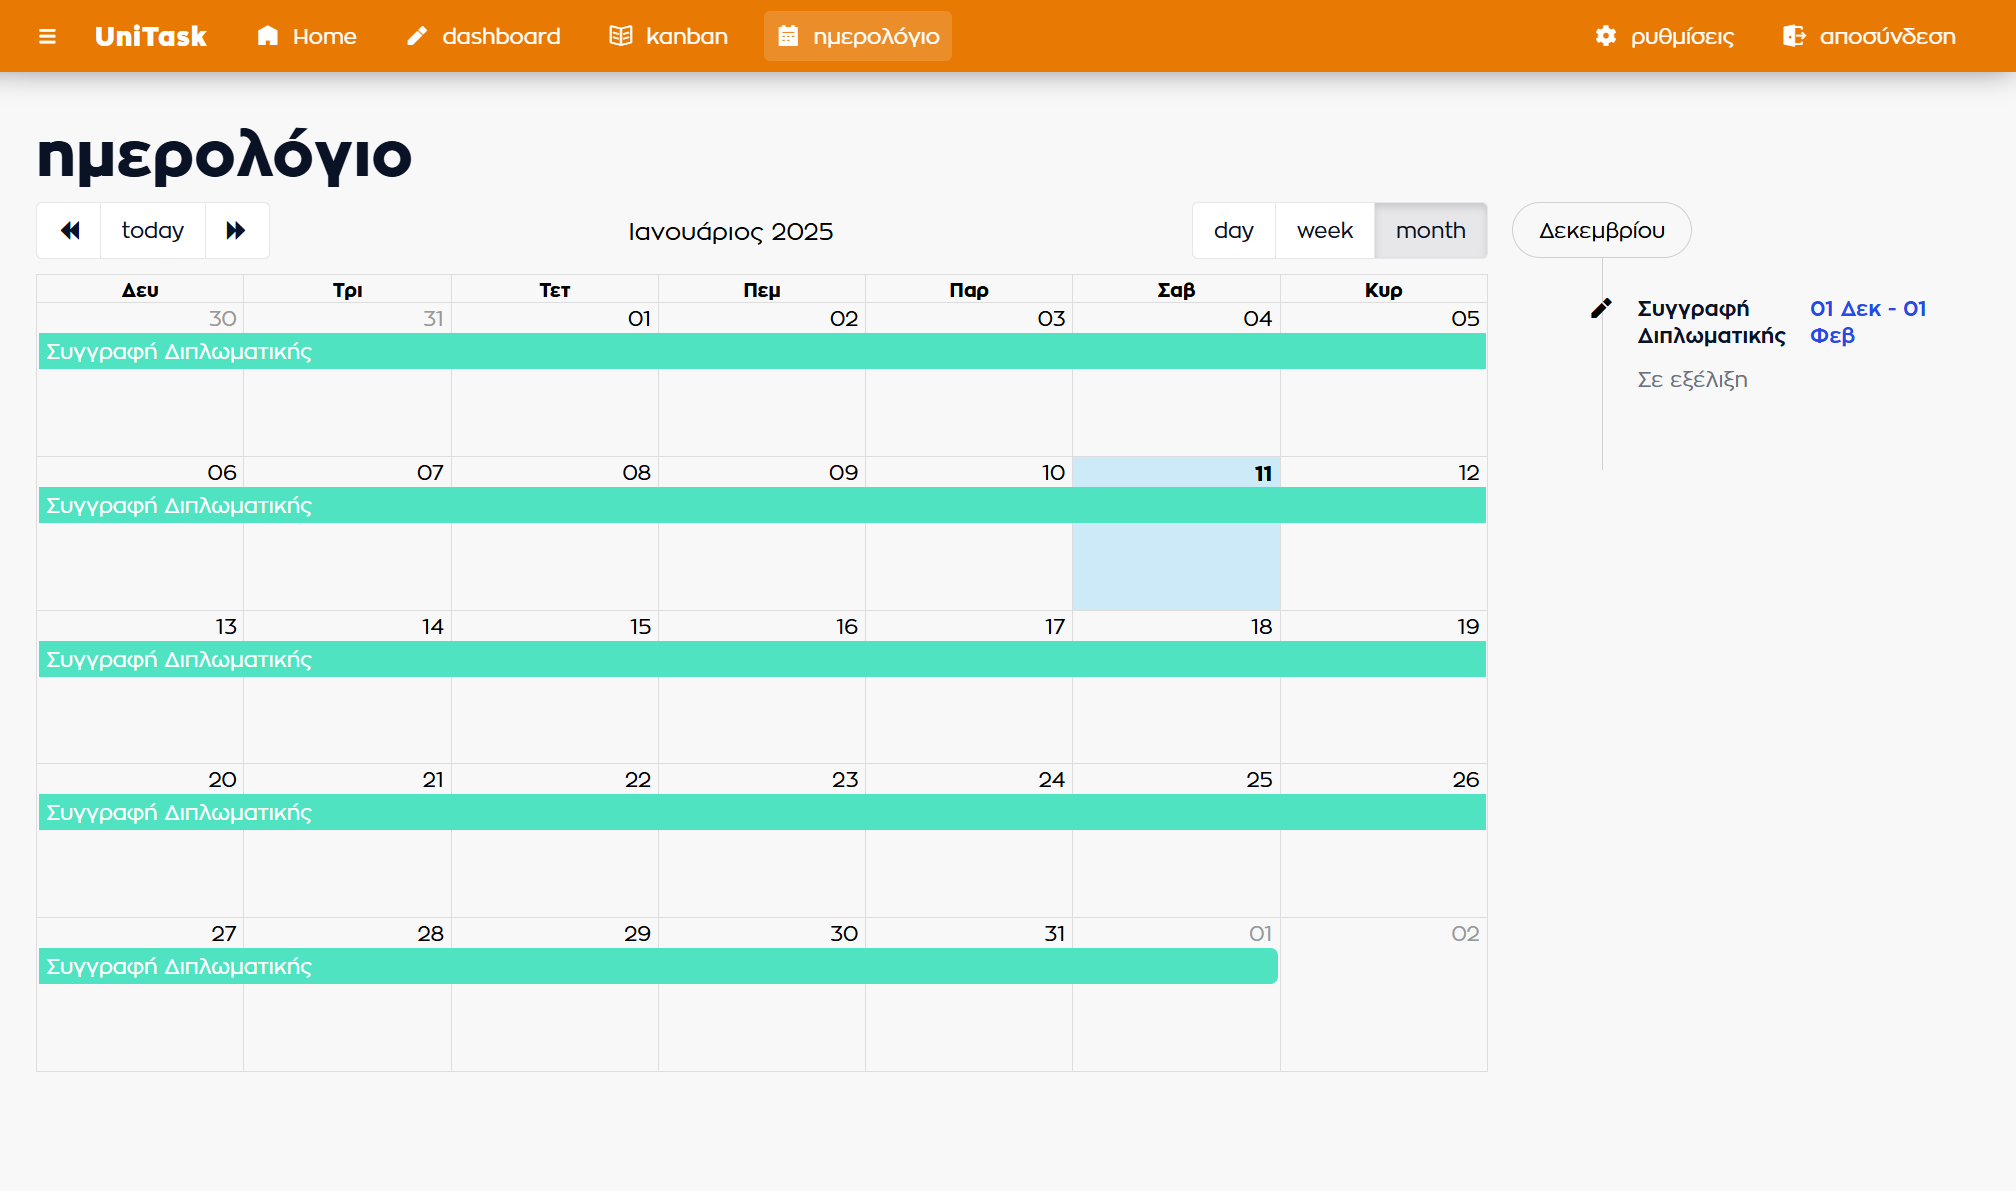
\includegraphics[width=\textwidth]{UniTask/Calendar_WithTask}
            \caption{\centering Σελίδα Calendar}
            \label{fig:unitask_Calendar_WithTask}
        \end{figure}

        Η σελίδα {\ZonaSB ρυθμίσεις} (σχήμα \ref{fig:unitask_Settings}) παρέχει επιλογές για τη μαζική διαγραφή εργασιών ή την ενεργοποίηση της λειτουργίας γρήγορης διαγραφής. Αυτή η λειτουργία εισάγει ένα κουμπί διαγραφής στις κάρτες εργασιών στο dashboard, επιτρέποντας την άμεση διαγραφή των εργασιών που θέλουμε χωρίς να χρειάζεται να μεταβούμε στη σελίδα επεξεργασίας κάθε εργασίας (σχήμα \ref{fig:unitask_Dashboard_Kanban_Calendar_WithTasks}.1). Τέλος, παρέχεται η δυνατότητα αρχικοποίησης των εργασιών. Στην αρχικοποίηση διαγράφονται οι υπάρχουσες εργασίες του χρήστη και δημιουργούνται κάποιες προκαθορισμένες οι οποίες λειτουργούν ως ένα demo (σχήμα \ref{fig:unitask_Dashboard_Kanban_Calendar_WithTasks}).

        \begin{figure}[h!] \noindent \centering
            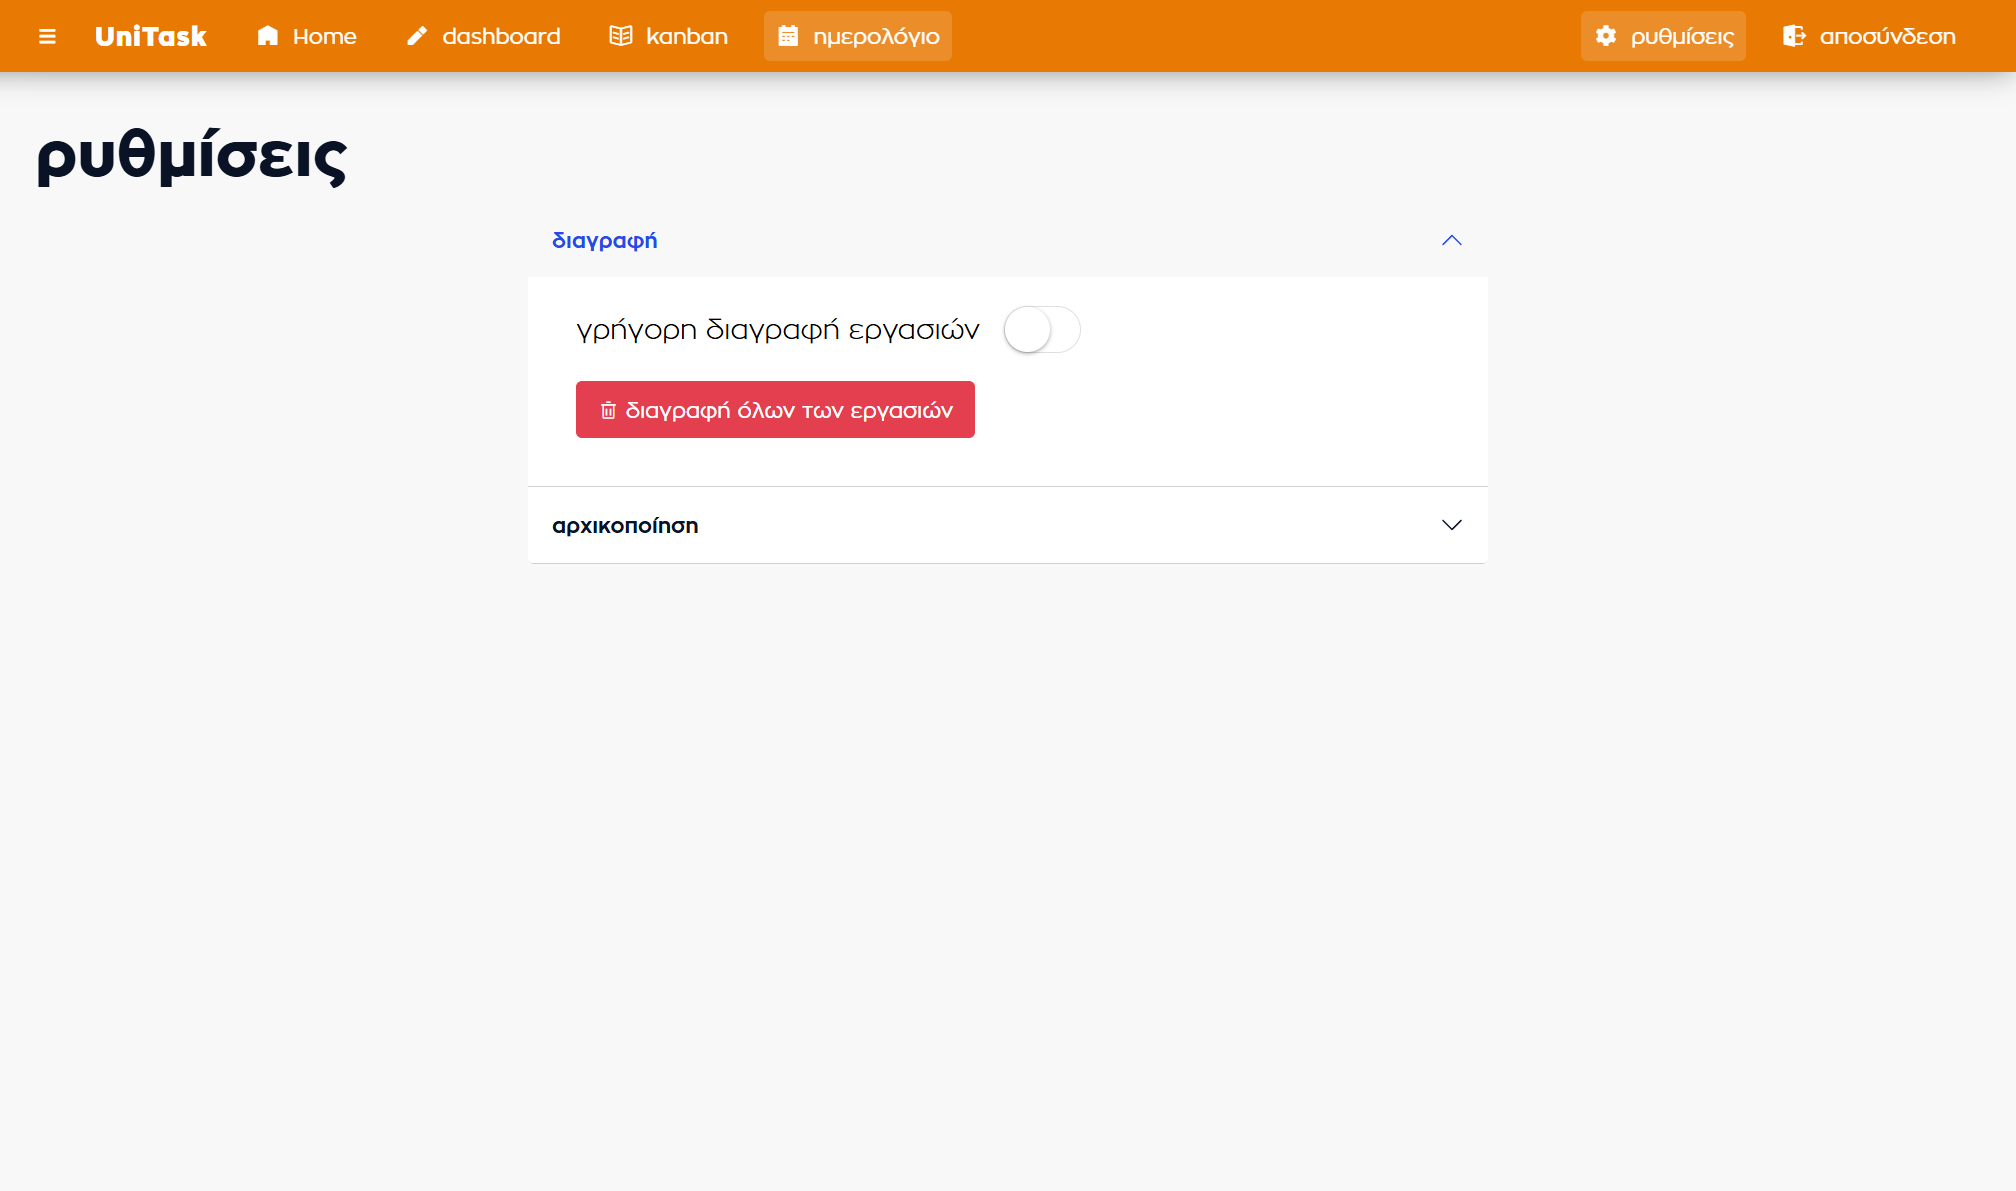
\includegraphics[trim={0 20cm 0 0}, clip, width=\textwidth]{UniTask/Settings_1}
            
\includegraphics[width=\textwidth]{UniTask/Settings_2}
            \caption{\centering Σελίδα ρυθμίσεων}
            \label{fig:unitask_Settings}
        \end{figure}

        Σε κάθε ρύθμιση εμφανίζονται επιβεβαιωτικά αναδυόμενα μηνύματα προκειμένου να αποφευχθούν ακούσιες διαγραφές εργασιών (σχήμα \ref{fig:unitask_InitializationPopUp}).

        \begin{figure}[h!] \noindent \centering
            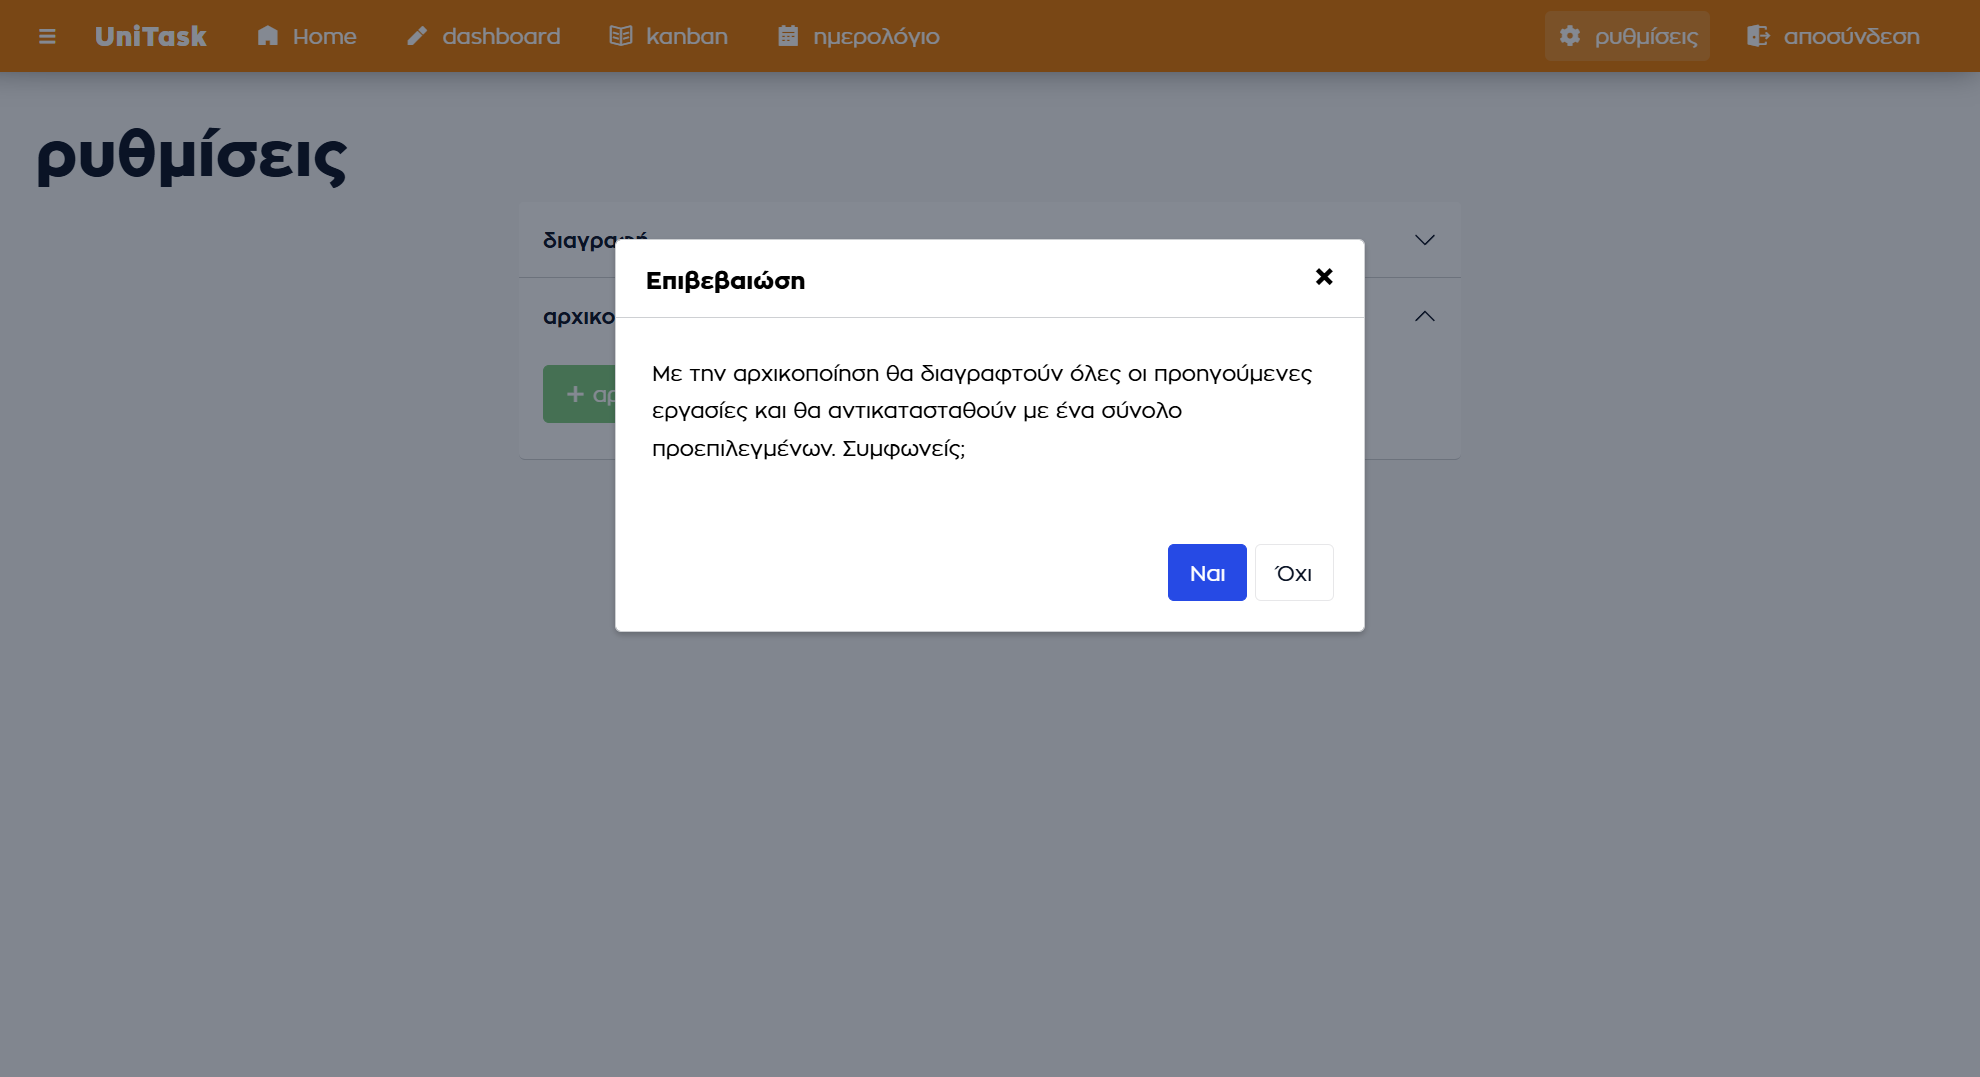
\includegraphics[trim={0 10cm 0 0}, clip, width=\textwidth]{UniTask/InitializationPopUp}
            \caption{\centering Σελίδα ρυθμίσεων}
            \label{fig:unitask_InitializationPopUp}
        \end{figure}

        \begin{figure}[p!] \noindent \centering
            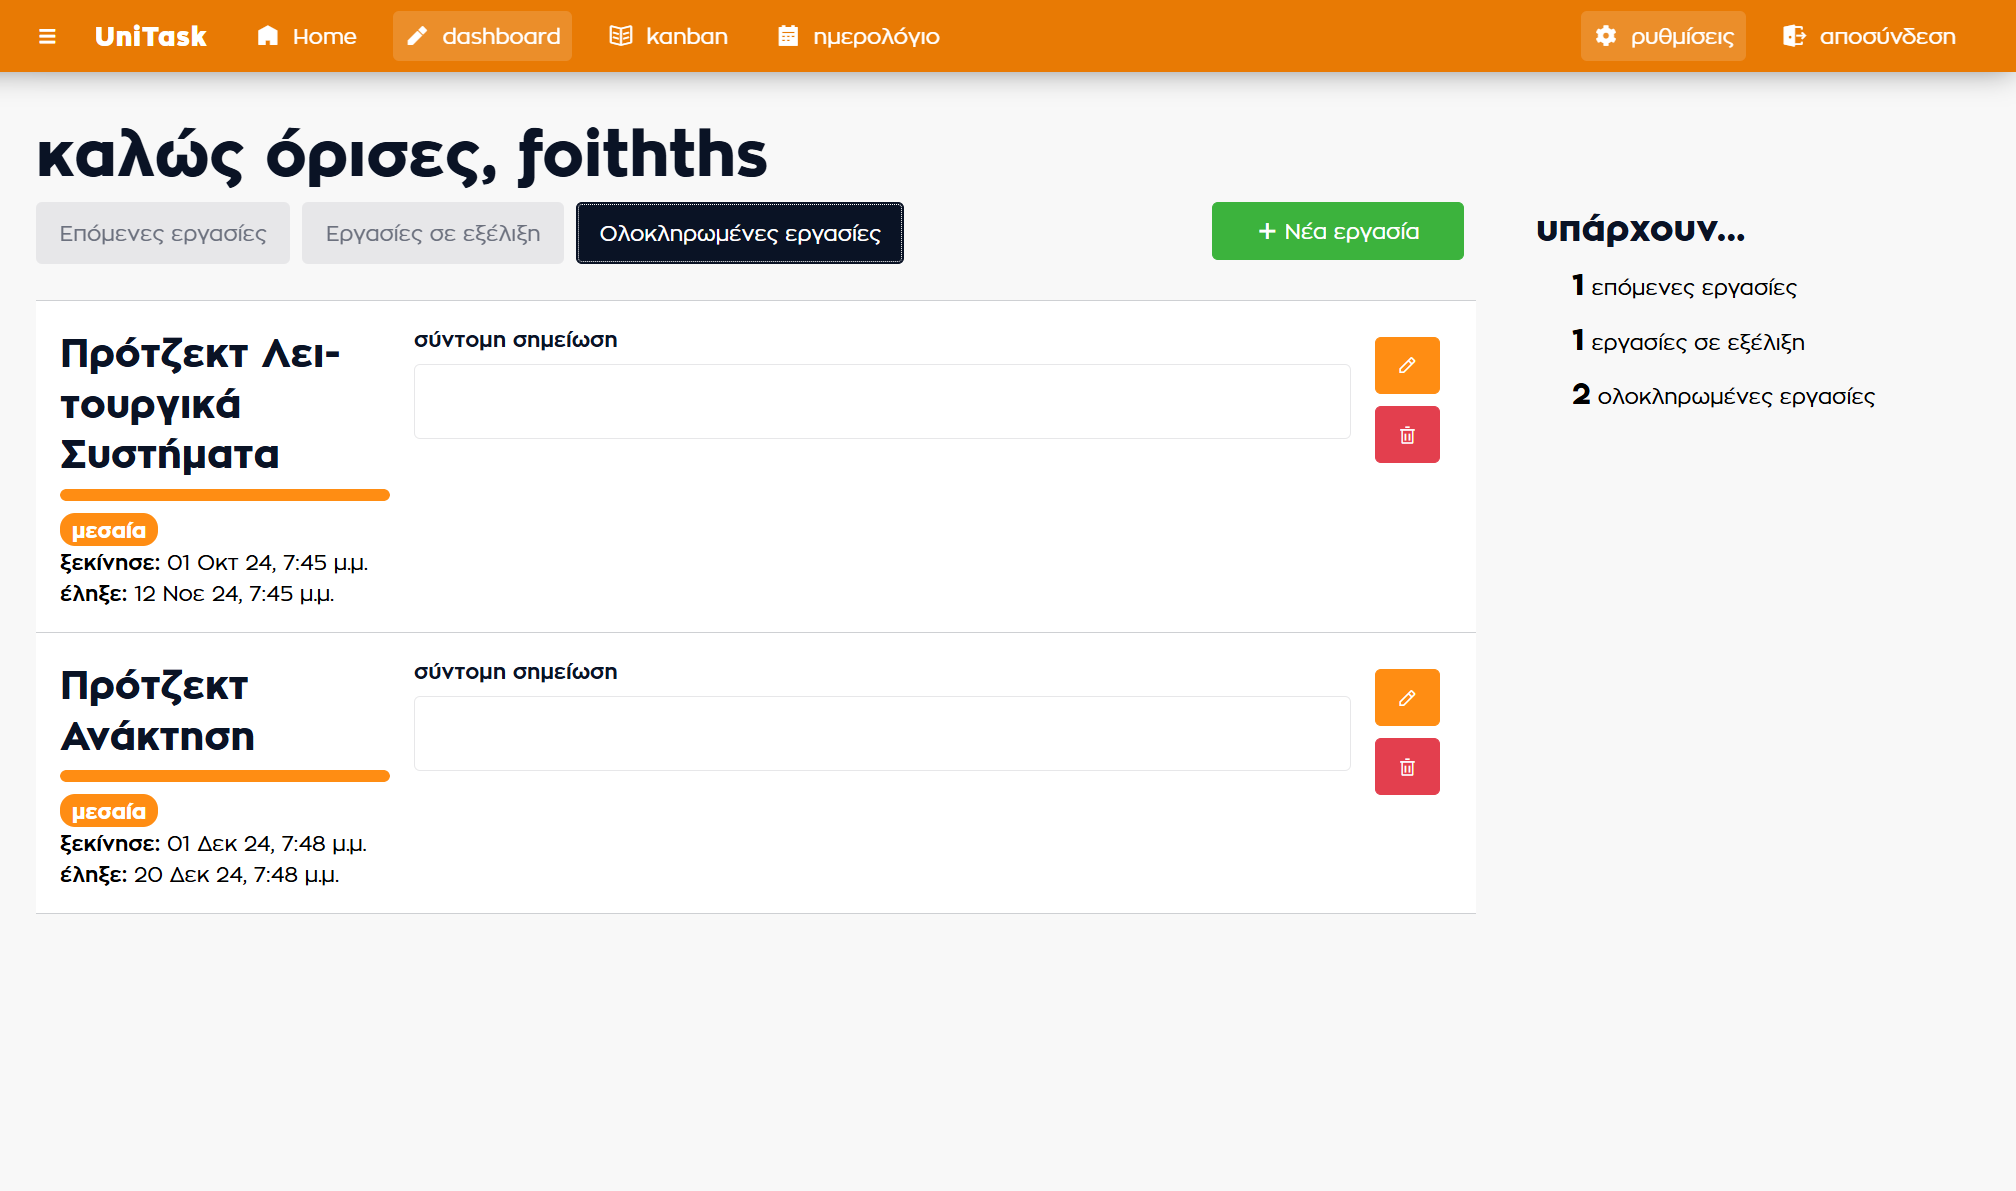
\includegraphics[trim={0 5cm 0 0}, clip, width=\textwidth]{UniTask/TaskDashboard_QuickDelete}
            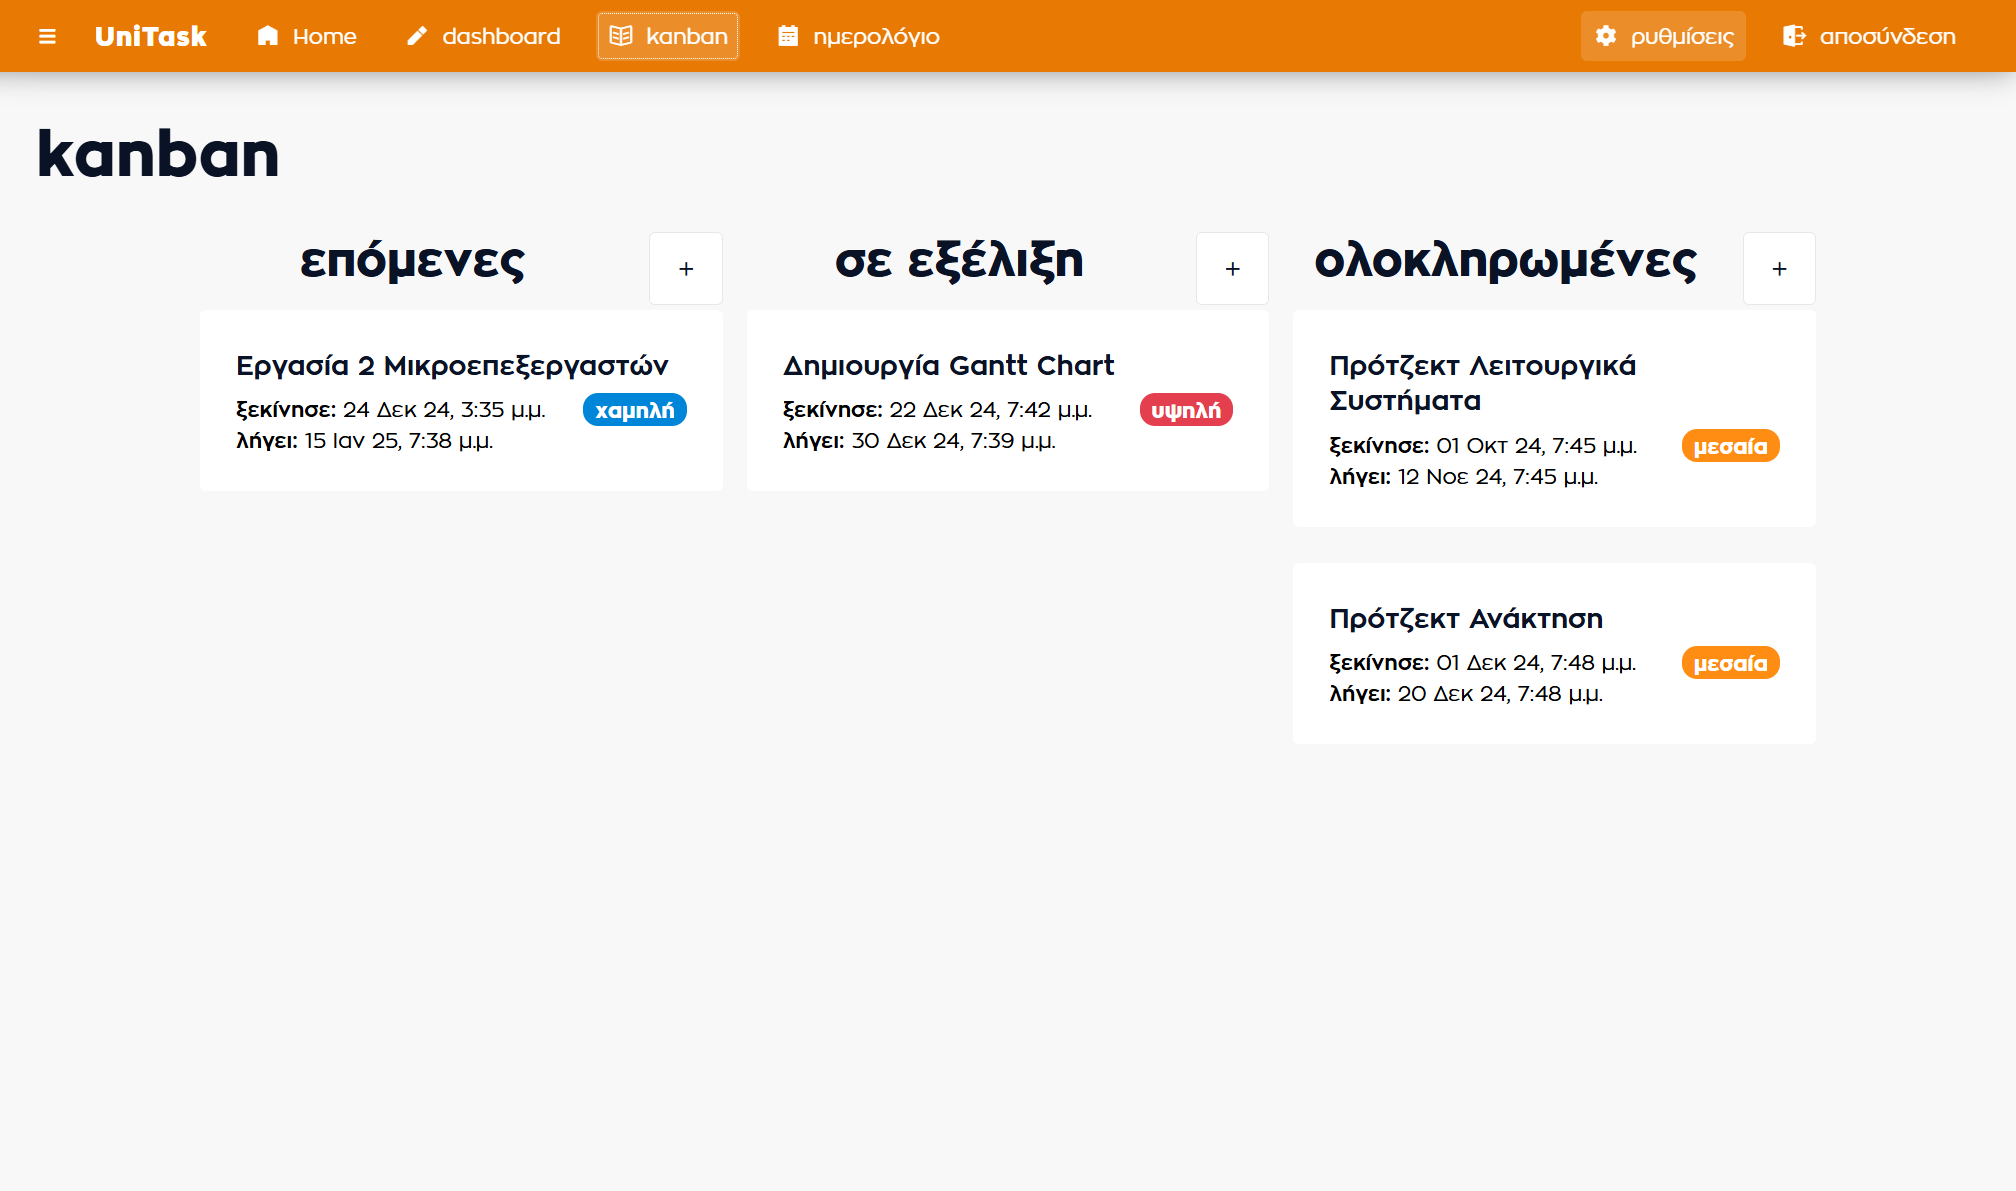
\includegraphics[trim={0 10cm 0 0}, clip, width=\textwidth]{UniTask/Kanban_WithTasks}
            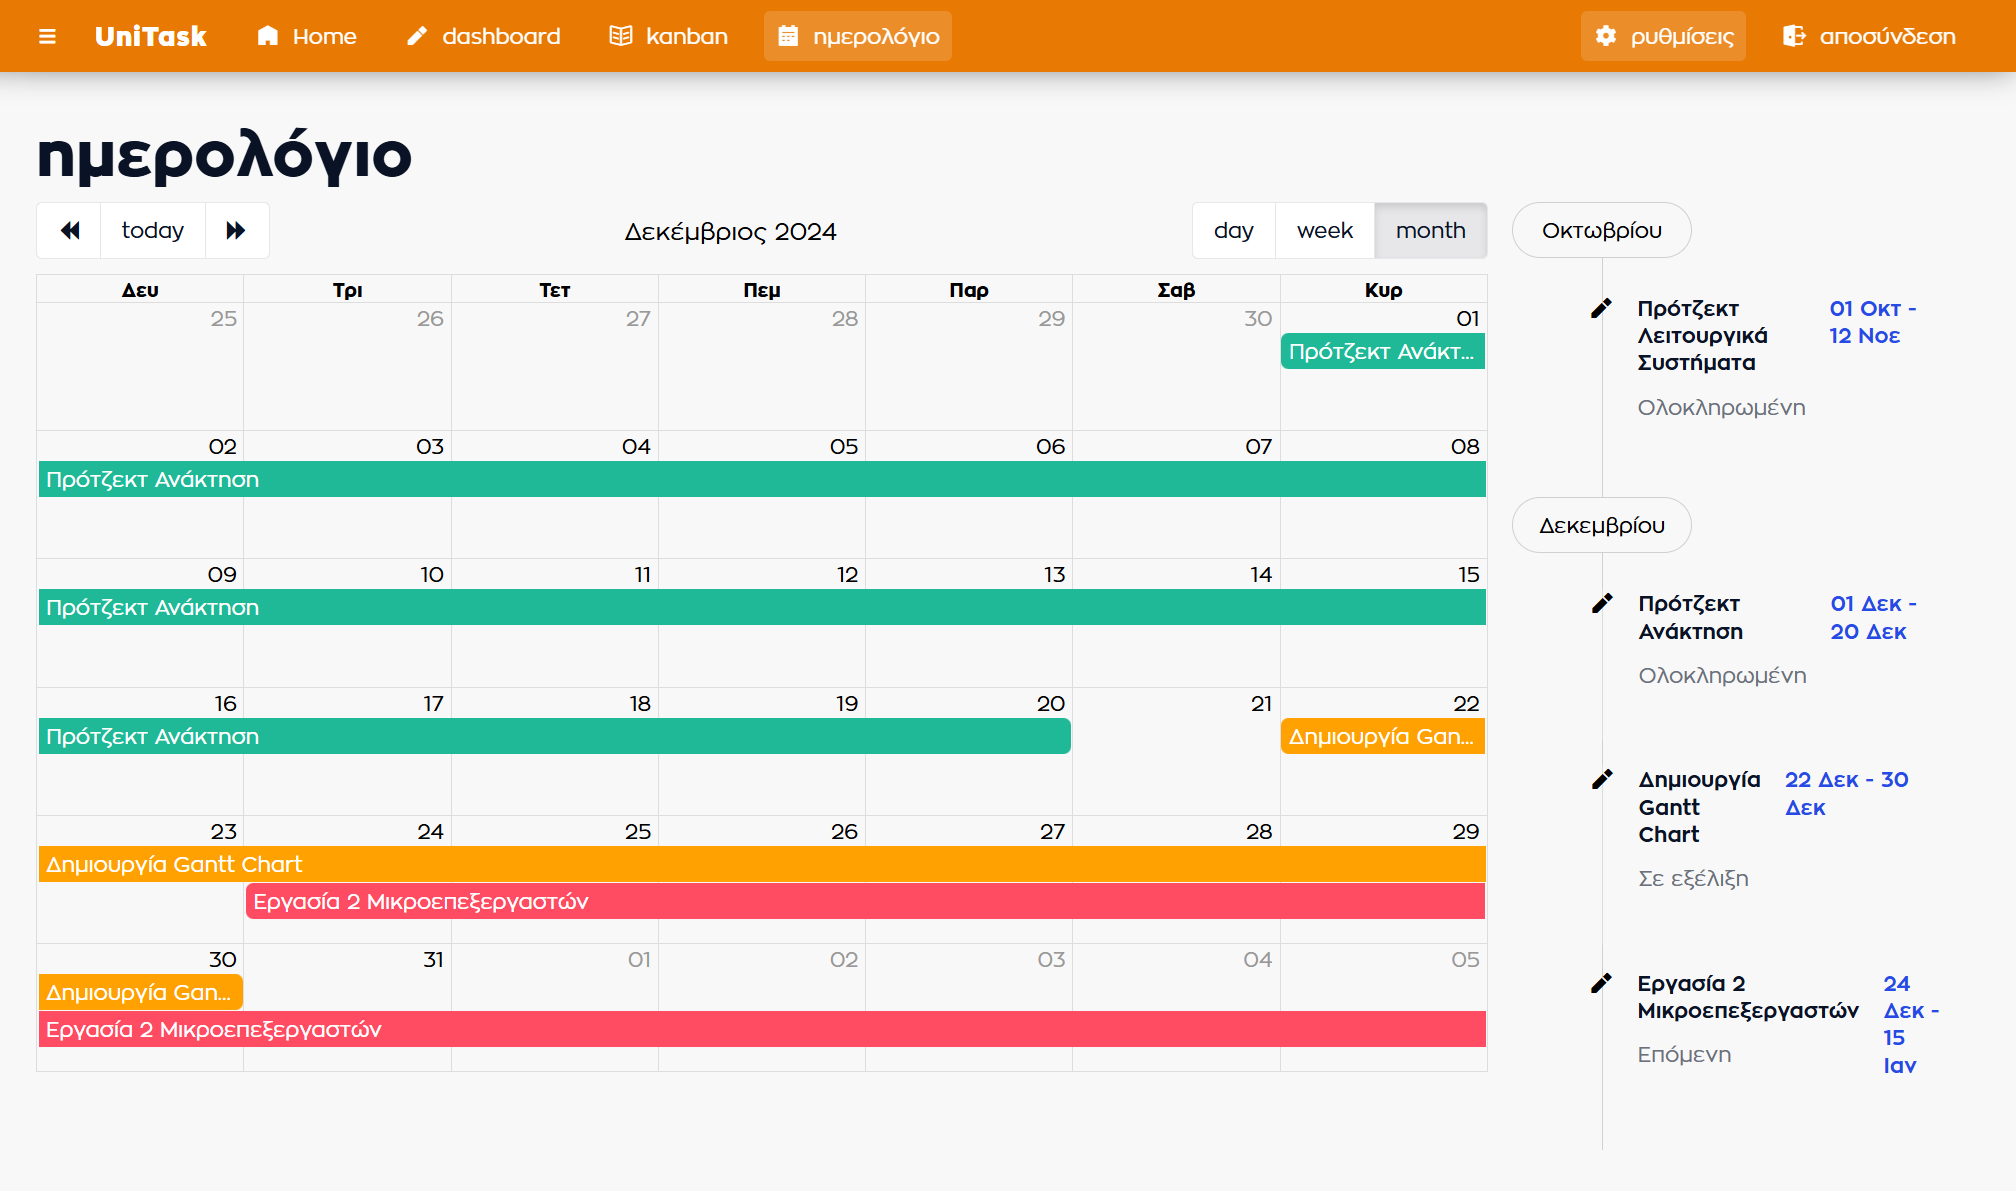
\includegraphics[width=\textwidth]{UniTask/Calendar_WithTasks}
            \caption{\centering Οι σελίδες Dashboard, Kanban και Calendar μετά την αρχικοποίηση των εργασιών. Στο Dashboard φαίνεται η λειτουργία γρήγορης διαγραφής εργασιών.}
            \label{fig:unitask_Dashboard_Kanban_Calendar_WithTasks}
        \end{figure}

    \section{Δομή της εφαρμογής} \label{sec:unitask_mendix}
        Πέρα από τα προκατασκευασμένα modules του Mendix, η λειτουργικότητα της εφαρμογής έχει οργανωθεί σε τρία modules, το \texttt{Administrator}, το \texttt{TaskManager} και το \texttt{UniTask}.

        \subsection{Module \texttt{Administrator}}
            Το \texttt{Administrator} περιλαμβάνει τη λειτουργικότητα που αφορά τη διαχείριση των χρηστών της εφαρμογής. Όλες οι οντότητες του domain model, οι σελίδες και τα microflows του module έχουν δικαιώματα ανάγνωσης και εγγραφής από τον \texttt{Administrator} ρόλο, όπως ορίζεται στο \texttt{Security} της εφαρμογής.

            \subsubsection{Domain model του \texttt{Administrator}}
                \begin{center}
                    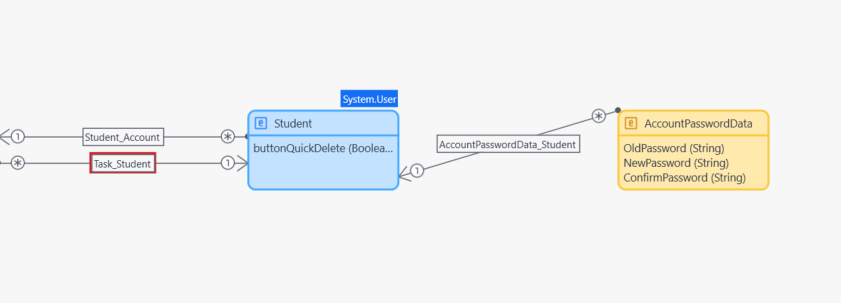
\includegraphics[width=\textwidth]{UniTask_Mendix/Administrator_DomainModel}
                \end{center}

                Το domain model του \texttt{Administrator} περιλαμβάνει την οντότητα \texttt{Student} που κληρονομεί την οντότητα \texttt{System.User} του Mendix. Η οντότητα περιγράφει τον κάθε χρήστη της εφαρμογής και περιλαμβάνει την Boolean ιδιότητα \texttt{buttonQuickDelete} αρχικοποιημένη σε \texttt{False} η οποία χρησιμοποιείται για την ενεργοποίηση της λειτουργίας γρήγορης διαγραφής εργασιών. Η οντότητα \texttt{Student} συσχετίζεται με την οντότητα \texttt{Account} του \texttt{System.User} με σχέση 1-προς-1, η οντότητα \texttt{Task} του \texttt{TaskManager} με σχέση ένα-προς-πολλά (ένα Student συσχετίζεται με πολλά Tasks) και την οντότητα \texttt{AccountPasswordData} με σχέση 1-προς-πολλά (ένα Student συσχετίζεται με πολλά AccountPasswordData).

                Η οντότητα \texttt{AccountPasswordData} είναι μη-διατηρήσιμη οντότητα (δεν αποθηκεύεται στη βάση δεδομένων αλλά μόνο στη μνήμη) και περιλαμβάνει τις ιδιότητες \texttt{OldPassword}, \texttt{NewPassword} και \texttt{ConfirmPassword} και χρησιμοποιείται για την αλλαγή του κωδικού πρόσβασης του χρήστη.

            \subsubsection{Σελίδες του \texttt{Administrator}}
                Στο \texttt{Administrator} περιλαμβάνονται οι εξής σελίδες:

                \begin{figure}[H] \noindent
                    \paragraph{\texttt{Account\_Overview}}
                    \begin{center}
                        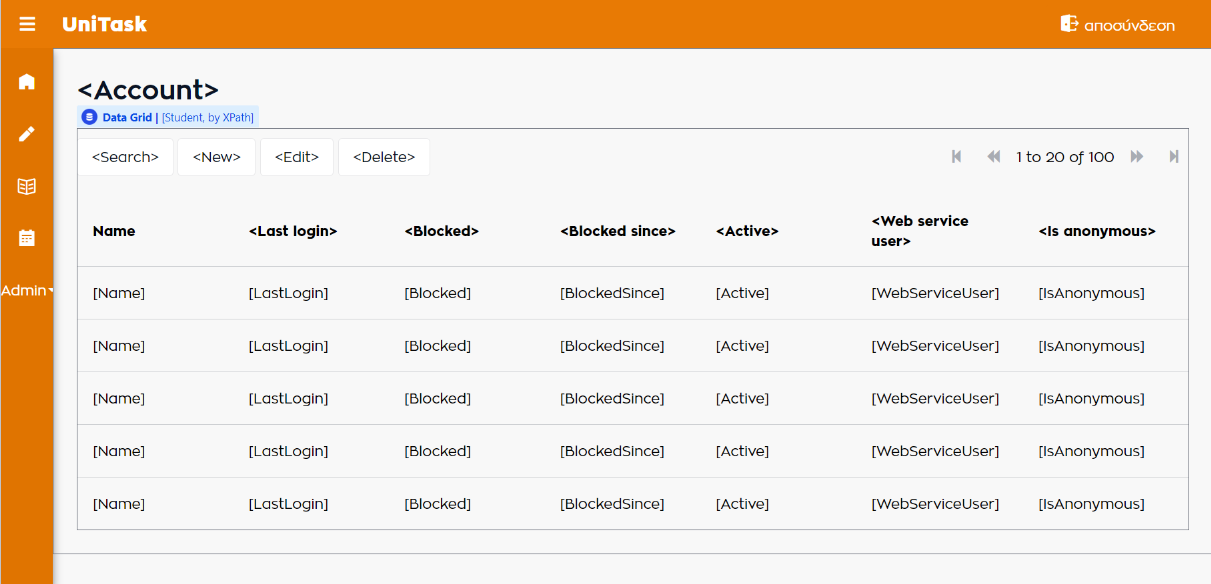
\includegraphics[width=\textwidth]{UniTask_Mendix/Account_Overview}
                    \end{center}
                \end{figure}

                    Η σελίδα χρησιμοποιείται για τη διαχείριση των χρηστών της εφαρμογής από την πλευρά των διαχειριστών.

                    Χρησιμοποιείται το \texttt{UniTask\_SideBar} layout του \texttt{UniTaskDesignSystem} module. Το κύριο μέρος της σελίδας αποτελείται από ένα Data Grid με Data source την οντότητα \texttt{Student} και με στήλες τις ιδιότητες \texttt{Name}, \texttt{Last login}, \texttt{Blocked}, \texttt{Blocked since}, \texttt{Active}, \texttt{Web service user} και \texttt{Is anonymous}.

                \begin{figure}[H] \noindent
                    \paragraph{\texttt{Account\_New}}
                    \begin{center}
                        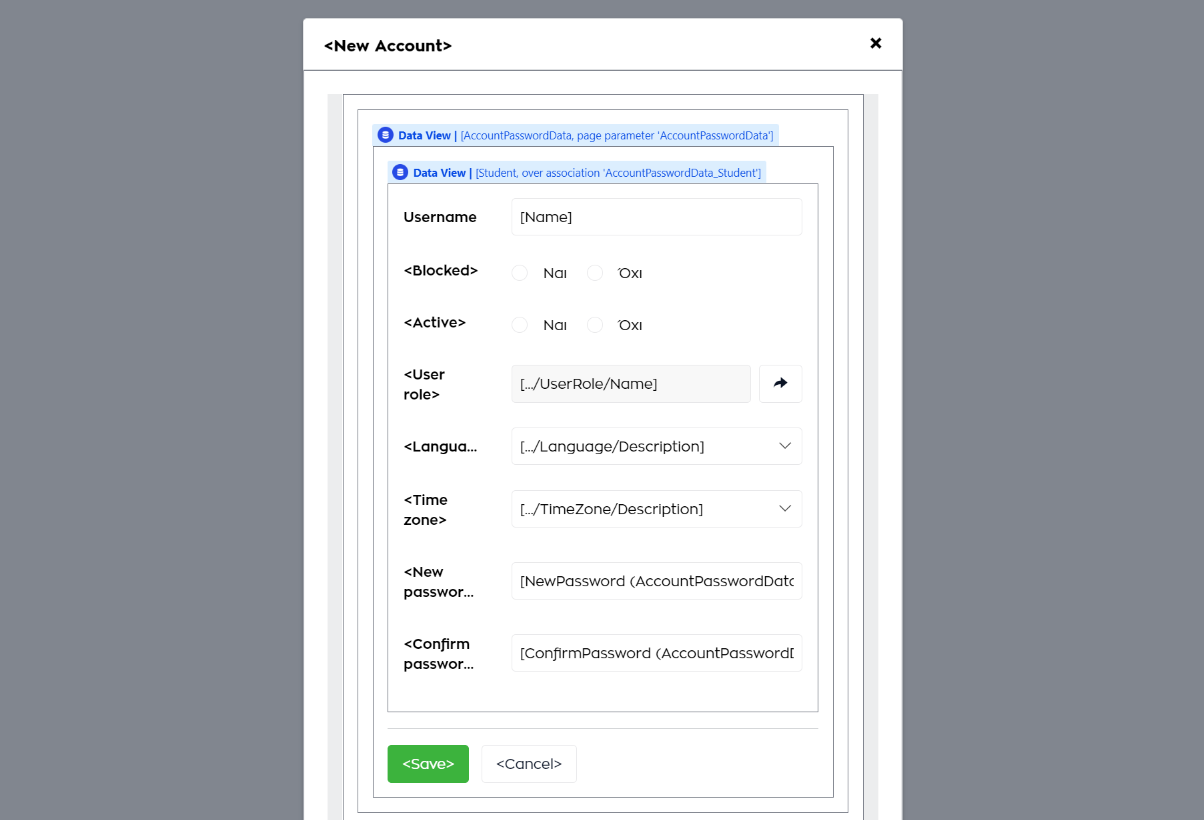
\includegraphics[width=\textwidth]{UniTask_Mendix/Account_New}
                    \end{center}
                \end{figure}

                    Η σελίδα χρησιμοποιείται για τη δημιουργία νέων χρηστών της εφαρμογής.

                    Χρησιμοποιείται το \texttt{PopupLayout} layout του \texttt{Atlas\_Core} module. Η σελίδα περιλαμβάνει δύο Parameters, το \texttt{Student} και \texttt{AccountPasswordData} του module \linebreak \texttt{Administrator}. Η σελίδα αποτελείται από δύο εμφωλευμένα Data Views, το εξωτερικό έχει ως Data source το \texttt{AccountPasswordData}, ενώ το εσωτερικό έχει ως Data source τη συσχέτιση του \texttt{AccountPasswordData} με το \texttt{Student}. Η χρήση του \texttt{AccountPasswordData} είναι απαραίτητη καθώς η δημιουργία ενός νέου χρήστη χρειάζεται την αποθήκευση του κωδικού πρόσβασής του.

                    Στο εσωτερικό Data View περιλαμβάνει Text Boxes, Radio Buttons και Input \linebreak Reference Set Selectors όπου εισάγονται τιμές για τα \texttt{Username}, \texttt{Blocked}, \texttt{Active}, \texttt{User role}, \texttt{Language}, \texttt{Time zone}, \texttt{New password} και \texttt{Confirm password}. Έχει σημασία να σημειωθεί πως οι ιδιότητες (γνωρίσματα) που αποθηκεύουμε στην πραγματικότητα δεν είναι ιδιότητες του \texttt{Student} αλλά του \texttt{System.User} του οποίου αποτελεί παιδί. Το Input Reference Set Selector χρησιμοποιείται για την επιλογή του \texttt{UserRole}, που αποτελεί διαφορετική σελίδα που θα αναλυθεί στη συνέχεια.

                    Τέλος, περιλαμβάνεται κουμπί για την αποθήκευση, το οποίο καλεί το microflow \texttt{ACT\_Account\_Save} του \texttt{Administrator} για την αποθήκευση των τιμών, και κουμπί για την ακύρωση της διαδικασίας.

                \begin{figure}[H] \noindent
                    \paragraph{\texttt{Account\_Edit}}
                    \begin{center}
                        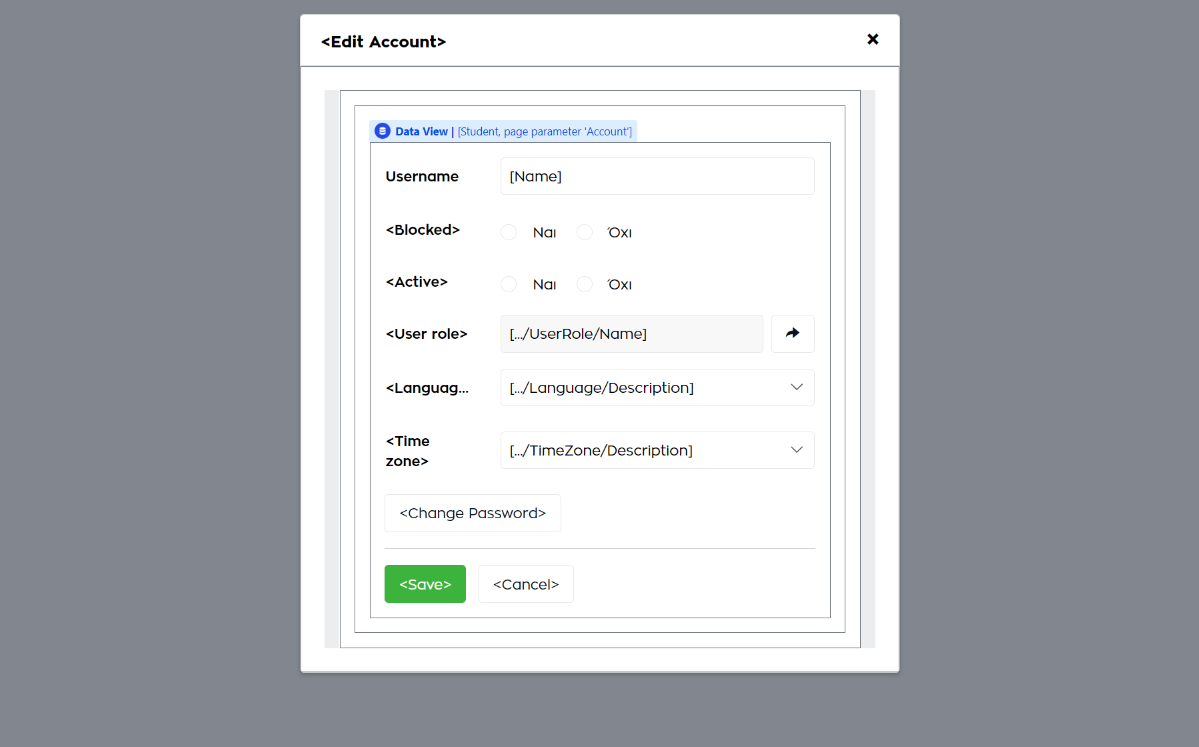
\includegraphics[width=\textwidth]{UniTask_Mendix/Account_Edit}
                    \end{center}
                \end{figure}

                    Η σελίδα χρησιμοποιείται για την επεξεργασία υπαρχόντων χρηστών της εφαρμογής.

                    Χρησιμοποιείται το \texttt{PopupLayout}. Η σελίδα περιλαμβάνει το Parameter \texttt{Student}. Η σελίδα αποτελείται από ένα Data View με Data source το \texttt{Student} με παρόμοια Text Boxes και Radio Buttons όπως και το \texttt{Account\_New}. Επίσης, περιλαμβάνεται το κουμπί που καλεί το microflow \texttt{ACT\_Password\_Change} για την αλλαγή κωδικού.

                    Τέλος, περιλαμβάνεται κουμπί για την αποθήκευση και κουμπί για την ακύρωση της διαδικασίας. Τα κουμπιά καλούν προεπιλεγμένες ενέργειες του Mendix.

                \begin{figure}[H] \noindent
                    \paragraph{\texttt{Change\_Password}}
                    \begin{center}
                        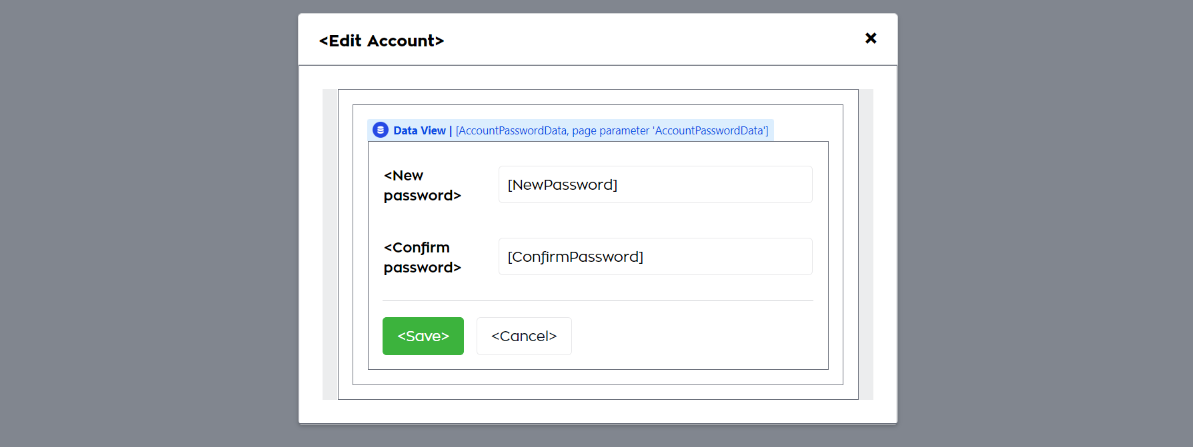
\includegraphics[width=\textwidth]{UniTask_Mendix/Change_Password}
                    \end{center}
                \end{figure}

                    Η σελίδα χρησιμοποιείται για την αλλαγή του κωδικού πρόσβασης υπάρχοντος χρήστη.

                    Χρησιμοποιείται το \texttt{PopupLayout}. Η σελίδα περιλαμβάνει το Parameter \linebreak \texttt{AccountPasswordData}, ένα Data View με Data source το \texttt{Student} με τα απαραίτητα Text Boxes για την αλλαγή των τιμών. Τέλος, περιλαμβάνεται κουμπί για την αποθήκευση που καλεί το microflow \texttt{ChangePassword} του \texttt{Administrator} και κουμπί για την ακύρωση της διαδικασίας.

                \begin{figure}[H] \noindent
                    \paragraph{\texttt{UserRole\_Select}}
                    \begin{center}
                        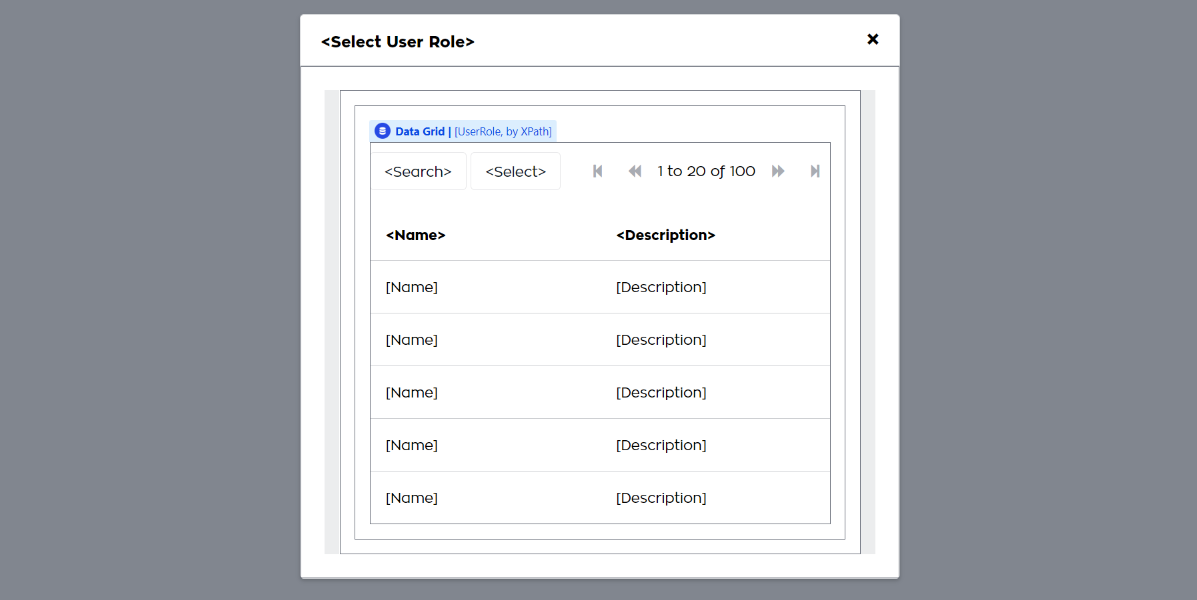
\includegraphics[width=\textwidth]{UniTask_Mendix/UserRole_Select}
                    \end{center}
                \end{figure}

                    Η σελίδα χρησιμοποιείται για την επιλογή του ρόλου του χρήστη κατά τη δημιουργία νέου χρήστη.

                    Χρησιμοποιείται το \texttt{PopupLayout}. Η σελίδα αποτελείται από ένα Data Grid με Data source το \texttt{UserRole} του \texttt{System}.\footnote{Τεχνικά, λόγω των ρόλων χρηστών που έχουν κληρονομηθεί από το Mendix περιλαμβάνεται και ο ρόλος Guest, ο οποίος στην πράξη δε χρησιμοποιείται καθώς έχει πρόσβαση μόνο στη σελίδα σύνδεσης.}

            \subsubsection{Microflows του \texttt{Administrator}}
                Στο \texttt{Administrator} περιλαμβάνονται τα εξής microflows:

                \begin{figure}[H] \noindent
                    \paragraph{\texttt{VAL\_Account}}
                    \begin{center}
                        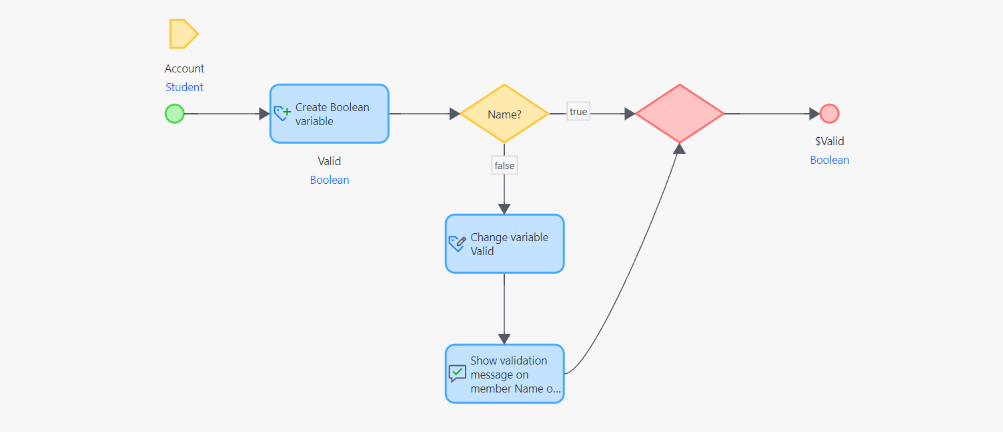
\includegraphics[width=\textwidth]{UniTask_Mendix/VAL_Account}
                    \end{center}
                \end{figure}

                    To microflow καλείται από το microflow \texttt{ACT\_Account\_Save} για να επικυρώσει τον λογαριασμό του χρήστη πριν αποθηκευτούν οι τιμές του.\footnote{Το πρόθεμα \texttt{VAL} χρησιμοποιείται στην ονομασία των microflows για να δηλώσει επικύρωση (validation).}

                    Αρχικά δημιουργείται μια boolean μεταβλητή \texttt{Valid} με αρχική τιμή \texttt{True} η οποία θα επιστραφεί από το microflow. Στη συνέχεια ελέγχεται αν για το αντικείμενο \texttt{Account} τύπου \texttt{Student} ισχύει η συνθήκη (\verb|trim($Account/Name) != ''|). Η έκφραση στη συνθήκη αφού καθαρίσει τα κενά (whitespaces) από το \texttt{Name} του \texttt{Account}, ελέγχει αν είναι διαφορετικό από το κενό string. Αν η συνθήκη δεν ισχύει, τότε η μεταβλητή \texttt{Valid} γίνεται \texttt{False}, η οποία επιστρέφεται μαζί με ένα popout μήνυμα. Αν η συνθήκη ισχύει, δηλαδή αν υπάρχει όνομα, τότε επιστρέφεται \texttt{True}.

                \begin{figure}[H] \noindent
                    \paragraph{\texttt{ACT\_Account\_New}}
                    \begin{center}
                        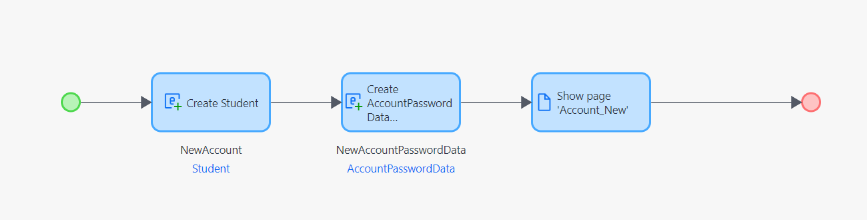
\includegraphics[width=\textwidth]{UniTask_Mendix/ACT_Account_New}
                    \end{center}
                \end{figure}

                    To microflow καλείται από τη σελίδα \texttt{Account\_Overview} με σκοπό τη δημιουργία ενός νέου χρήστη.\footnote{Το πρόθεμα \texttt{ACT} χρησιμοποιείται στην ονομασία των microflows για να δηλώσει μια ενέργεια (action).}

                    Αρχικά δημιουργούνται δύο στιγμιότυπα τύπου \texttt{Student} και \texttt{AccountPasswordData} με ονόματα \texttt{NewAccount} και \texttt{NewAccountPasswordData} αντίστοιχα. Να σημειωθεί πως το \texttt{NewAccountPasswordData} συσχετίζεται με το \texttt{Student}. Τα αντικείμενα δε γίνονται commit ακόμα στη βάση, καθώς είναι κενά. Στη συνέχεια εμφανίζεται η σελίδα \texttt{Account\_New} με τα αντικείμενα \texttt{NewAccount} και \texttt{NewAccountPasswordData} ως Parameters.

                \begin{figure}[H] \noindent
                    \paragraph{\texttt{ACT\_Account\_Save}}
                    \begin{center}
                        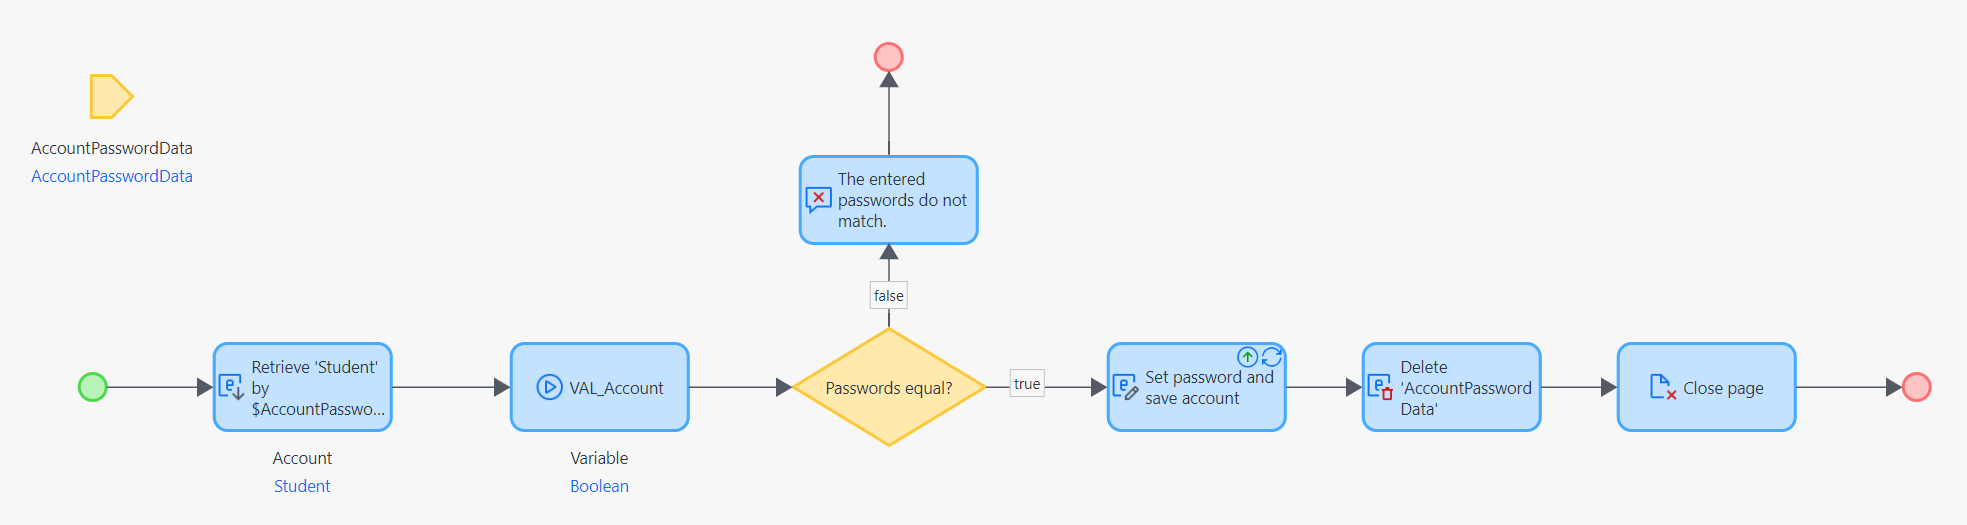
\includegraphics[width=\textwidth]{UniTask_Mendix/ACT_Account_Save}
                    \end{center}
                \end{figure}

                    To microflow καλείται από τη σελίδα \texttt{Account\_New} με σκοπό την αποθήκευση των τιμών του νέου χρήστη.

                    Το microflow έχει ως Parameter το \texttt{AccountPasswordData}. Μαζί με αυτό, ανακτάται το \texttt{Student} αφού συσχετίζονται, και καλείται το microflow \texttt{VAL\_Account} το οποίο ελέγχει αν το \texttt{Name} του \texttt{Student} είναι κενό. Αν το \texttt{Name} είναι κενό, τότε εμφανίζεται ένα popout μήνυμα και το microflow τερματίζεται. Αν το \texttt{Name} δεν είναι κενό, τότε ελέγχεται αν το \texttt{NewPassword} του \texttt{AccountPasswordData} είναι ίσο με το \texttt{ConfirmPassword}, όπως έχουν δοθεί στη φόρμα \texttt{Account\_New}. Αν η συνθήκη δεν ισχύει, τότε εμφανίζεται ένα popout μήνυμα και το microflow τερματίζεται. Αν η συνθήκη ισχύει, τότε το \texttt{NewPassword} γίνεται commit στο \texttt{Account} τύπου \texttt{Student} στο γνώρισμα \texttt{Password} το οποίο είναι Hashed string. Στη συνέχεια το αντικείμενο \texttt{AccountPasswordData} διαγράφεται και κλείνει η σελίδα.

                \begin{figure}[H] \noindent
                    \paragraph{\texttt{ACT\_Account\_Edit}}
                    \begin{center}
                        
\includegraphics[width=\textwidth]{UniTask_Mendix/ACT_Account_Edit}
                    \end{center}
                \end{figure}

                    To microflow καλείται από τη σελίδα \texttt{Account\_Overview} με σκοπό την επεξεργασία ενός υπάρχοντος χρήστη.

                    Το microflow εμφανίζει τη σελίδα \texttt{Account\_Edit} με το \texttt{Account} τύπου \texttt{Student} ως Parameter.

                \begin{figure}[H] \noindent
                    \paragraph{\texttt{VAL\_Password}}
                    \begin{center}
                        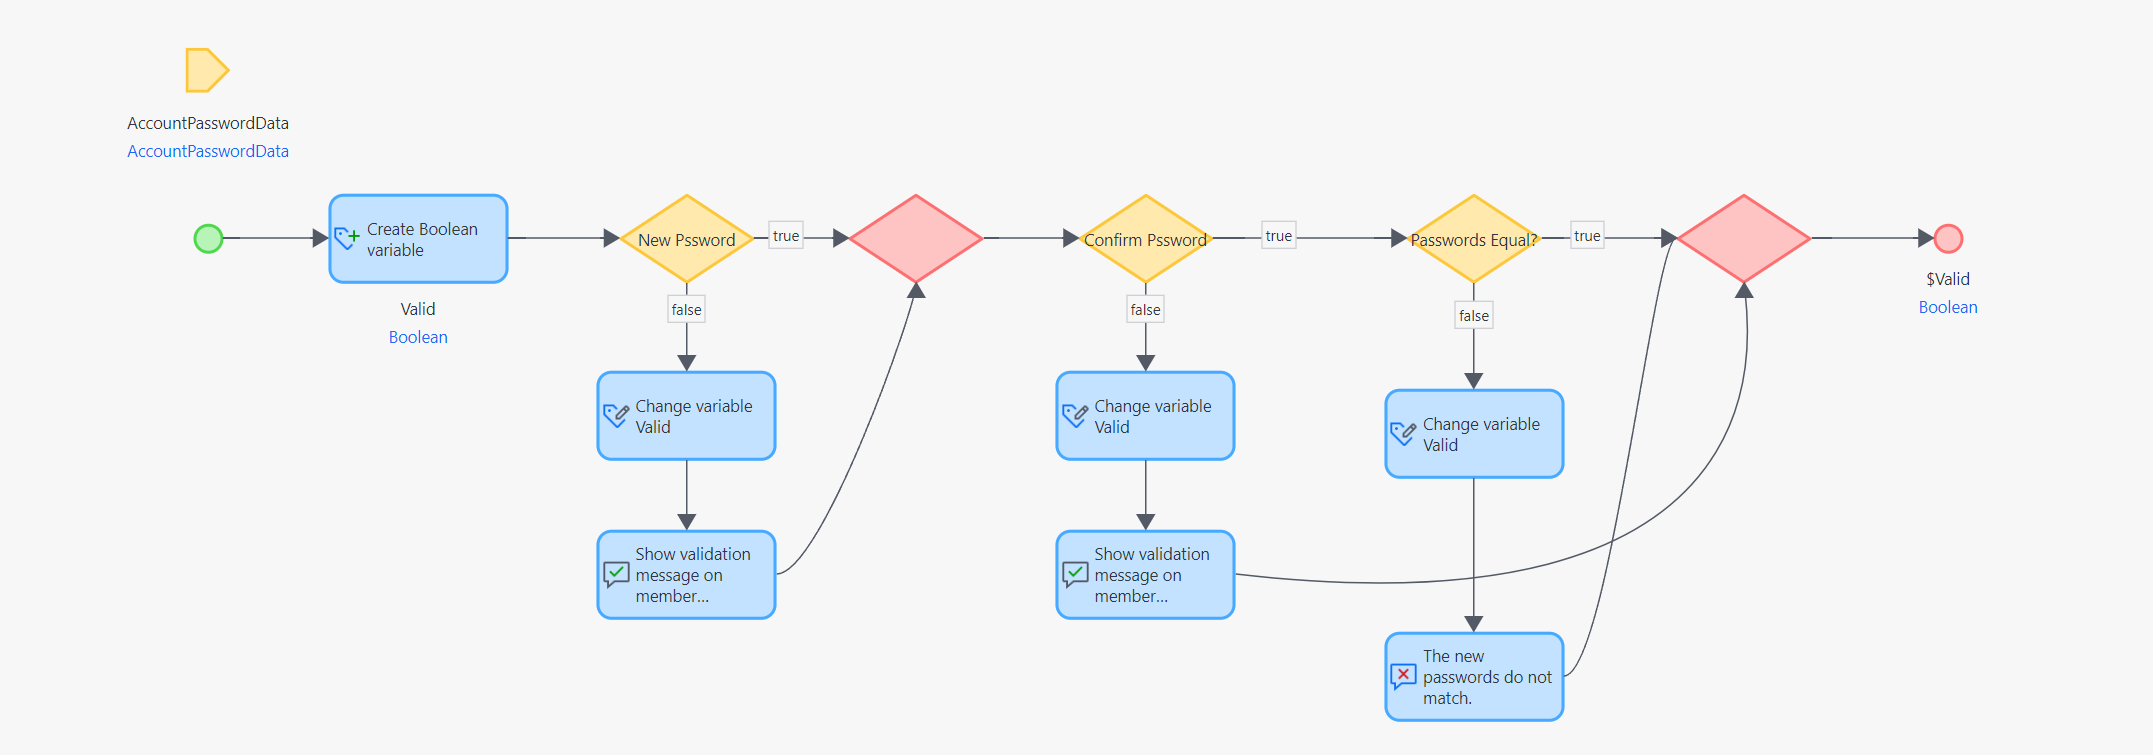
\includegraphics[width=\textwidth]{UniTask_Mendix/VAL_Password}
                    \end{center}
                \end{figure}

                    To microflow καλείται από το microflow \texttt{ChangePassword} με σκοπό τον έλεγχο των συνθηκών για την αλλαγή του κωδικού πρόσβασης.

                    Αρχικά δημιουργείται μια boolean μεταβλητή \texttt{Valid} με αρχική τιμή \texttt{True}. Στη συνέχεια ελέγχεται αν για το \texttt{NewPassword} του αντικειμένου \texttt{AccountPasswordData} ισχύει η συνθήκη (\verb|trim($AccountPasswordData/NewPassword) != ''|). Η έκφραση στη συνθήκη ελέγχει αν έχει δοθεί όντως νέος κωδικός στη φόρμα της σελίδας \texttt{Change\_Password}. Αν η συνθήκη ισχύει, ελέγχεται με παρόμοιο τρόπο και το \texttt{ConfirmPassword} όπως επίσης και το αν είναι ίσο με το \texttt{NewPassword}. Αν κάποια συνθήκη από τις προαναφερθείσες δεν ισχύει, η μεταβλητή \texttt{Valid} γίνεται \texttt{False} και εμφανίζεται κατάλληλο popout μήνυμα. Αν όλες οι συνθήκες ισχύουν, τότε η μεταβλητή \texttt{Valid} παραμένει \texttt{True} και επιστρέφεται από το microflow.

                \begin{figure}[H] \noindent
                    \paragraph{\texttt{ChangePassword}}
                    \begin{center}
                        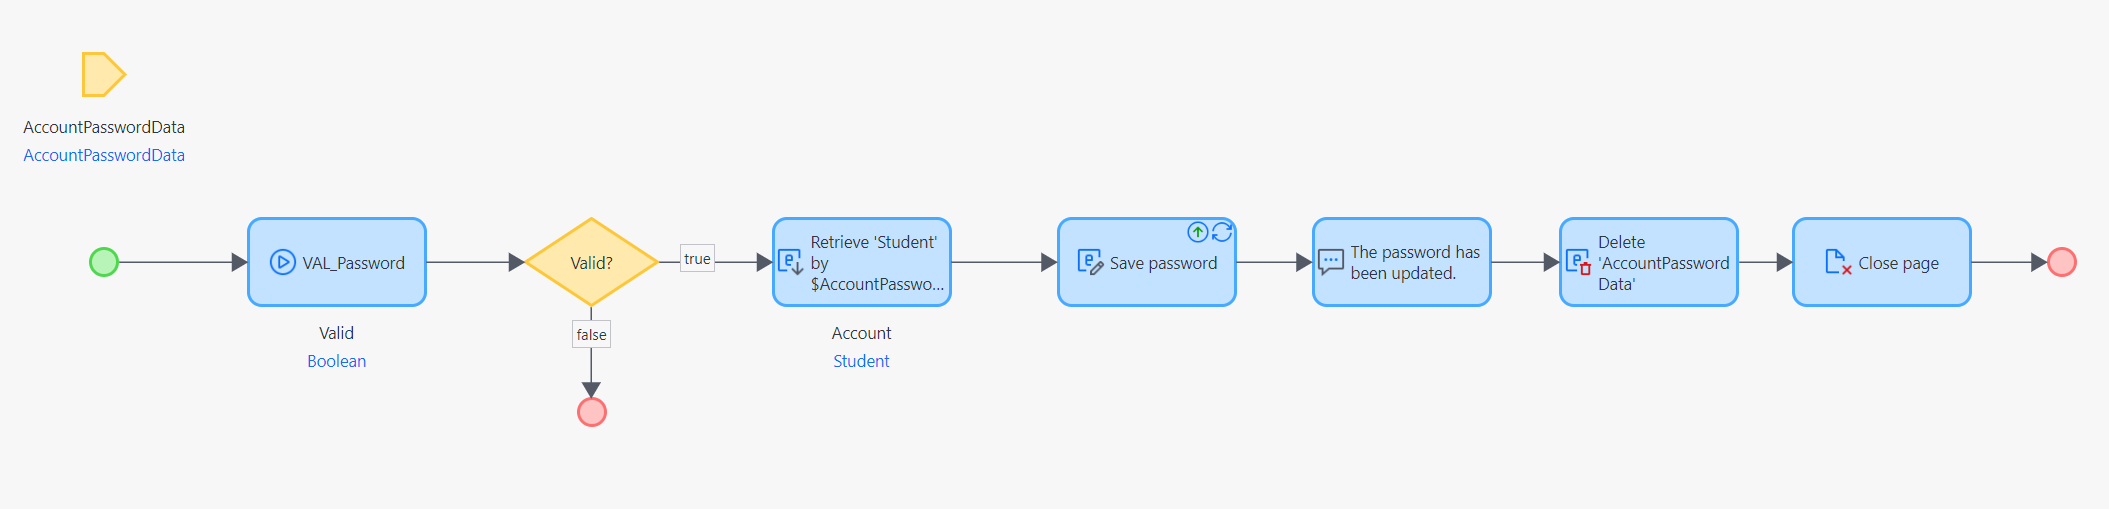
\includegraphics[width=\textwidth]{UniTask_Mendix/ChangePassword}
                    \end{center}
                \end{figure}

                    To microflow καλείται από τη σελίδα \texttt{Change\_Password} με σκοπό την αποθήκευση του νέου κωδικού πρόσβασης για έναν υπάρχων χρήστη.

                    Το microflow έχει ως Parameter το \texttt{AccountPasswordData}. Στην αρχή καλείται το microflow \texttt{VAL\_Password} για τον έλεγχο των συνθηκών. Αν η μεταβλητή \texttt{Valid} που επιστρέφεται από το microflow είναι \texttt{False}, τότε το microflow τερματίζεται. Αν είναι \texttt{True}, τότε γίνεται retrieve και το αντικείμενο \texttt{Student} ως συσχέτιση, γίνεται commit το \texttt{NewPassword} ως Hashed string \texttt{Password} στο \texttt{Student}, εμφανίζεται κατάλληλο popout μήνυμα, διαγράφεται το \texttt{AccountPasswordData} και κλείνει η σελίδα.

                \begin{figure}[H] \noindent
                    \paragraph{\texttt{ACT\_Password\_Change}}
                    \begin{center}
                        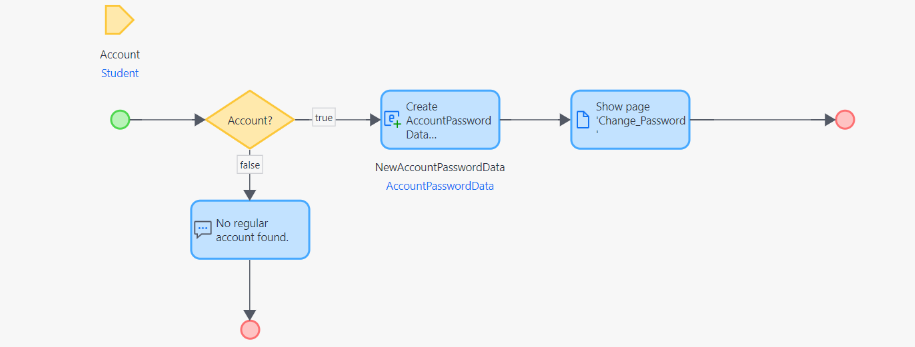
\includegraphics[width=\textwidth]{UniTask_Mendix/ACT_Password_Change}
                    \end{center}
                \end{figure}

                    To microflow καλείται από τη σελίδα \texttt{Account\_Edit} με σκοπό την αλλαγή του κωδικού πρόσβασης ενός υπάρχοντος χρήστη.

                    Με Parameter το \texttt{Account} τύπου \texttt{Student}, αρχικά ελέγχεται αν υπάρχει όντως κάποιο υπαρκτό \texttt{Account}. Αν δεν υπάρχει, εμφανίζεται popout μήνυμα και το microflow τερματίζεται. Αν υπάρχει, τότε δημιουργείται ένα νέο αντικείμενο \texttt{AccountPasswordData} συσχετισμένο με το \texttt{Account} και εμφανίζεται η σελίδα \texttt{Change\_Password} με το \linebreak \texttt{AccountPasswordData} και \texttt{Account} ως Parameters.

                \begin{figure}[H] \noindent
                    \paragraph{\texttt{ASU\_Administrator\_Create}}
                    \begin{center}
                        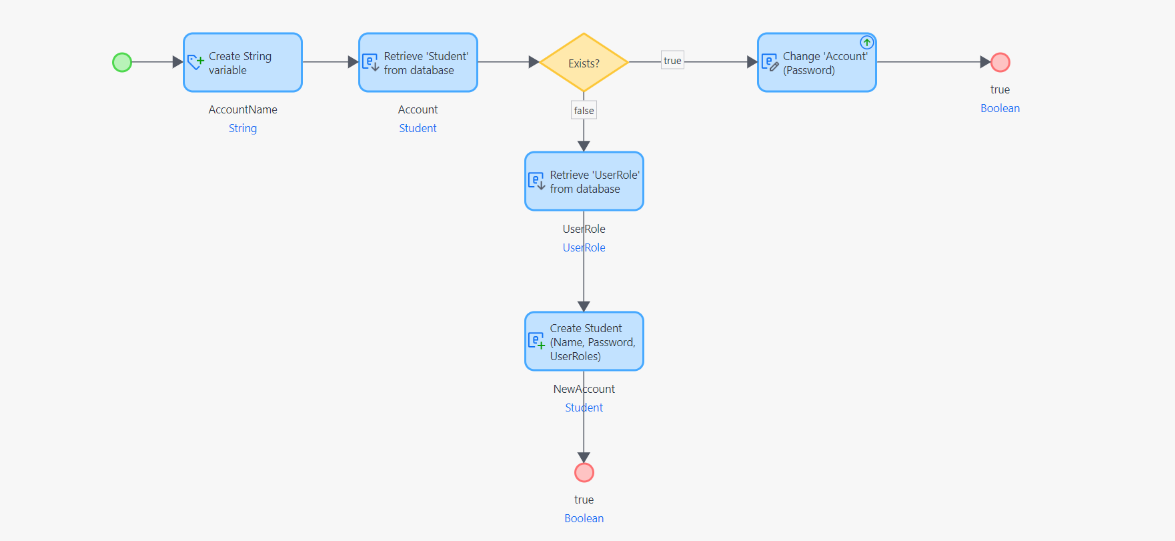
\includegraphics[width=\textwidth]{UniTask_Mendix/ASU_Administrator_Create}
                    \end{center}
                \end{figure}

                    Microflow που καλείται κατά την αρχικοποίηση της εφαρμογής για τη δημιουργία του διαχειριστή της εφαρμογής. \footnote{Το πρόθεμα \texttt{ASU} (After Startup) χρησιμοποιείται στην ονομασία των microflows για να δηλώσει ότι καλείται αμέσως μετά την εκκίνηση της εφαρμογής.}

                    Αρχικά δημιουργείται το String \texttt{AccountName} με τιμή \texttt{'admin'} με το username του διαχειριστή. Στη συνέχεια γίνεται retrieve από τη βάση δεδομένων το \texttt{Student} που έχει ως \texttt{Name} το \texttt{AccountName}. Αν δεν υπάρχει τέτοιος λογαριασμός, τότε γίνονται retrieve τα \texttt{System.UserRoles} και δημιουργείται ένα νέο αντικείμενο \texttt{Student} με \texttt{Name} το \texttt{AccountName}, \texttt{Password} η τιμή \texttt{'admin'} και \texttt{UserRole} το \texttt{UserRole}. Αν υπάρχει ήδη λογαριασμός με το \texttt{AccountName}, τότε αλλάζει ο κωδικός σε \texttt{'admin'}. Είναι προφανές ότι τα στοιχεία σύνδεσης του διαχειριστή έχουν οριστεί ως \texttt{'admin'} και \texttt{'admin'}.

        \subsection{Module \texttt{TaskManager}}
            Το \texttt{TaskManager} περιλαμβάνει τη λειτουργικότητα που αφορά τη διαχείριση των εργασιών της εφαρμογής. Όλες οι οντότητες του domain model, οι σελίδες και τα microflows του module έχουν δικαιώματα ανάγνωσης και εγγραφής από τον \texttt{User} ρόλο, όπως ορίζεται στο \texttt{Security} της εφαρμογής, με εξαίρεση το \texttt{Custom\_LogIn\_Page} που έχει δικαίωμα ο \texttt{Guest}.

            \subsubsection{Domain model του \texttt{TaskManager}}
                \begin{center}
                    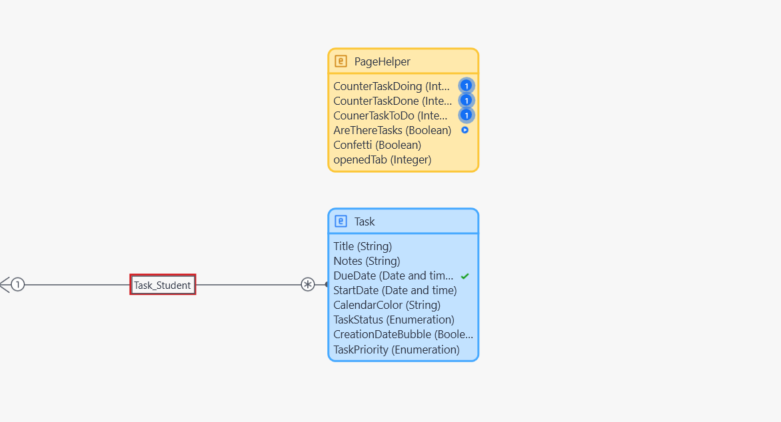
\includegraphics[width=\textwidth]{UniTask_Mendix/TaskManager_DomainModel}
                \end{center}

                Το domain model του \texttt{TaskManager} περιλαμβάνει την οντότητα \texttt{Task} και τη μη-διατηρήσιμη οντότητα \texttt{PageHelper}.

                Η οντότητα \texttt{Task} αναπαριστά την εκάστοτε εργασία του χρήστη της εφαρμογής. Περιλαμβάνει τις ιδιότητες \texttt{Title} τύπου String ως 200 χαρακτήρες με το όνομα της εργασίας, \texttt{Notes} τύπου String με απεριόριστους χαρακτήρες όπου μπορούν να προστεθούν σημειώσεις για αυτή και \texttt{DueDate} τύπου Date and time με την ημερομηνία λήξης. Επίσης, περιλαμβάνει τη \texttt{StartDate} τύπου Date and time με την ημερομηνία έναρξης, η οποία αρχικοποιείται με την τιμή \verb|'%CurrentDateTime%]'| (Token που επιστρέφει την τρέχουσα ημερομηνία και ώρα) και τη \texttt{CalendarColor} τύπου String που αποθηκεύει το χρώμα της εργασίας στο ημερολόγιο. Λόγω της φύσης του widget του ημερολογίου, το String θα έχει πάντα τη μορφή \texttt{'rgb(<0-255>, <0-255>, <0-255>)'} και στην οντότητα αρχικοποιείται με την τιμή \texttt{'rgb(38,74,229)'} που αντιστοιχεί στο μπλε χρώμα.

                Επιπλέον, η οντότητα περιλαμβάνει τις ιδιότητες \texttt{TaskStatus} και \texttt{TaskPriority} όπου είναι Enumeration ιδιότητες των Enumeration εγγράφων \texttt{TaskStatus} και \linebreak \texttt{TaskPriority}, αρχικοποιημένες με \texttt{To\_Do} και \texttt{Low} αντίστοιχα. Το \texttt{TaskStatus} καθορίζει την κατάσταση της εργασίας με τις δυνατές καταστάσεις να είναι \texttt{'To\_Do'}, \texttt{'Doing'} και \texttt{'Done'} ενώ το \texttt{TaskPriority} καθορίζει αν η προτεραιότητα της εργασίας είναι χαμηλή, μεσαία ή υψηλή. Επίσης, περιλαμβάνεται η ιδιότητα \texttt{CreationDateBubble} τύπου Boolean που αρχικοποιείται με \texttt{True}. Η ιδιότητα αυτή χρησιμοποιείται για την εμφάνιση ενός επεξηγηματικού μηνύματος στον χρήστη όταν δημιουργεί μια νέα εργασία. Να σημειωθεί επίσης πως το \texttt{DateDue} περιλαμβάνει ένα Validation rule που ελέγχει αν η ημερομηνία λήξης είναι μετά την ημερομηνία έναρξης \texttt{StartDate}, και αν δεν ισχύει, τότε εμφανίζεται κατάλληλο μήνυμα.

                Η οντότητα \texttt{PageHelper} περιλαμβάνει τις ιδιότητες \texttt{CounterTaskDoing}, \linebreak \texttt{CounterTaskDone} και \texttt{CounterTaskToDo} τύπου Integer, των οποίων οι τιμές καθορίζονται από τα microflows \texttt{CounterTaskDoing}, \texttt{CounterTaskDone} και \texttt{CounterTaskToDo} αντίστοιχα. Οι ιδιότητες αυτές χρησιμοποιούνται για την εμφάνιση των τριών μετρητών. Επίσης, περιλαμβάνει την Boolean ιδιότητα \texttt{AreThereTasks} που καθορίζεται από το microflow \texttt{AreThereTasks} και χρησιμεύει για την εμφάνιση του επεξηγηματικού παραθύρου στο Dashboard, την Boolean ιδιότητα \texttt{Confetti} που αρχικοποιείται με \texttt{False} και χρησιμοποιείται για την εμφάνιση του κομφετί (σύστημα επιβράβευσης), και τέλος την ιδιότητα \texttt{openedTab} τύπου Integer αρχικοποιημένη με μηδέν που χρησιμεύει για την αποθήκευση της τρέχουσας καρτέλας του Dashboard που έχει ανοίξει ο χρήστης.

            \subsubsection{Σελίδες του \texttt{TaskManager}}
                Στο \texttt{TaskManager} περιλαμβάνονται οι εξής σελίδες:

                \begin{figure}[H] \noindent
                    \paragraph{\texttt{Custom\_LogIn\_Overview}}
                    \begin{center}
                        
\includegraphics[width=\textwidth]{UniTask_Mendix/Custom_LogIn_Page}
                    \end{center}
                \end{figure}

                Η σελίδα χρησιμοποιείται για την είσοδο του χρήστη στην εφαρμογή. Πρόσβαση στη σελίδα έχουν μόνο οι \texttt{Guest} χρήστες.

                Χρησιμοποιείται το \texttt{Layout\_LogIn} layout του \texttt{UniTaskDesignSystem} module, με μια φόρμα που περιλαμβάνει τα Text Boxes για το \texttt{Username} και \texttt{Password} του χρήστη και το κουμπί για την είσοδο. Τα κουμπιά καλούν προεπιλεγμένες ενέργειες του Mendix.

                \begin{figure}[H] \noindent
                    \paragraph{\texttt{PAGE\_Home\_Page}}
                    \begin{center}
                        
\includegraphics[width=\textwidth]{UniTask_Mendix/PAGE_Home_Page}
                    \end{center}
                \end{figure}

                Η αρχική σελίδα της εφαρμογής που εμφανίζεται μετά την είσοδο του χρήστη.

                Η σελίδα χρησιμοποιεί το \texttt{UniTask\_TopBar} layout του \texttt{UniTaskDesignSystem} module, το οποίο εμφανίζει το κεντρικό μενού της εφαρμογής στο πάνω μέρος της σελίδας. Περιλαμβάνει το τίτλο {\ZonaSB UniTask} με ένα call to action κουμπί που καλεί το microflow \texttt{ShowPage\_TasksOverview}.

                \begin{figure}[H] \noindent
                    \paragraph{\texttt{PAGE\_Tasks\_Overview}}
                    \begin{center}
                        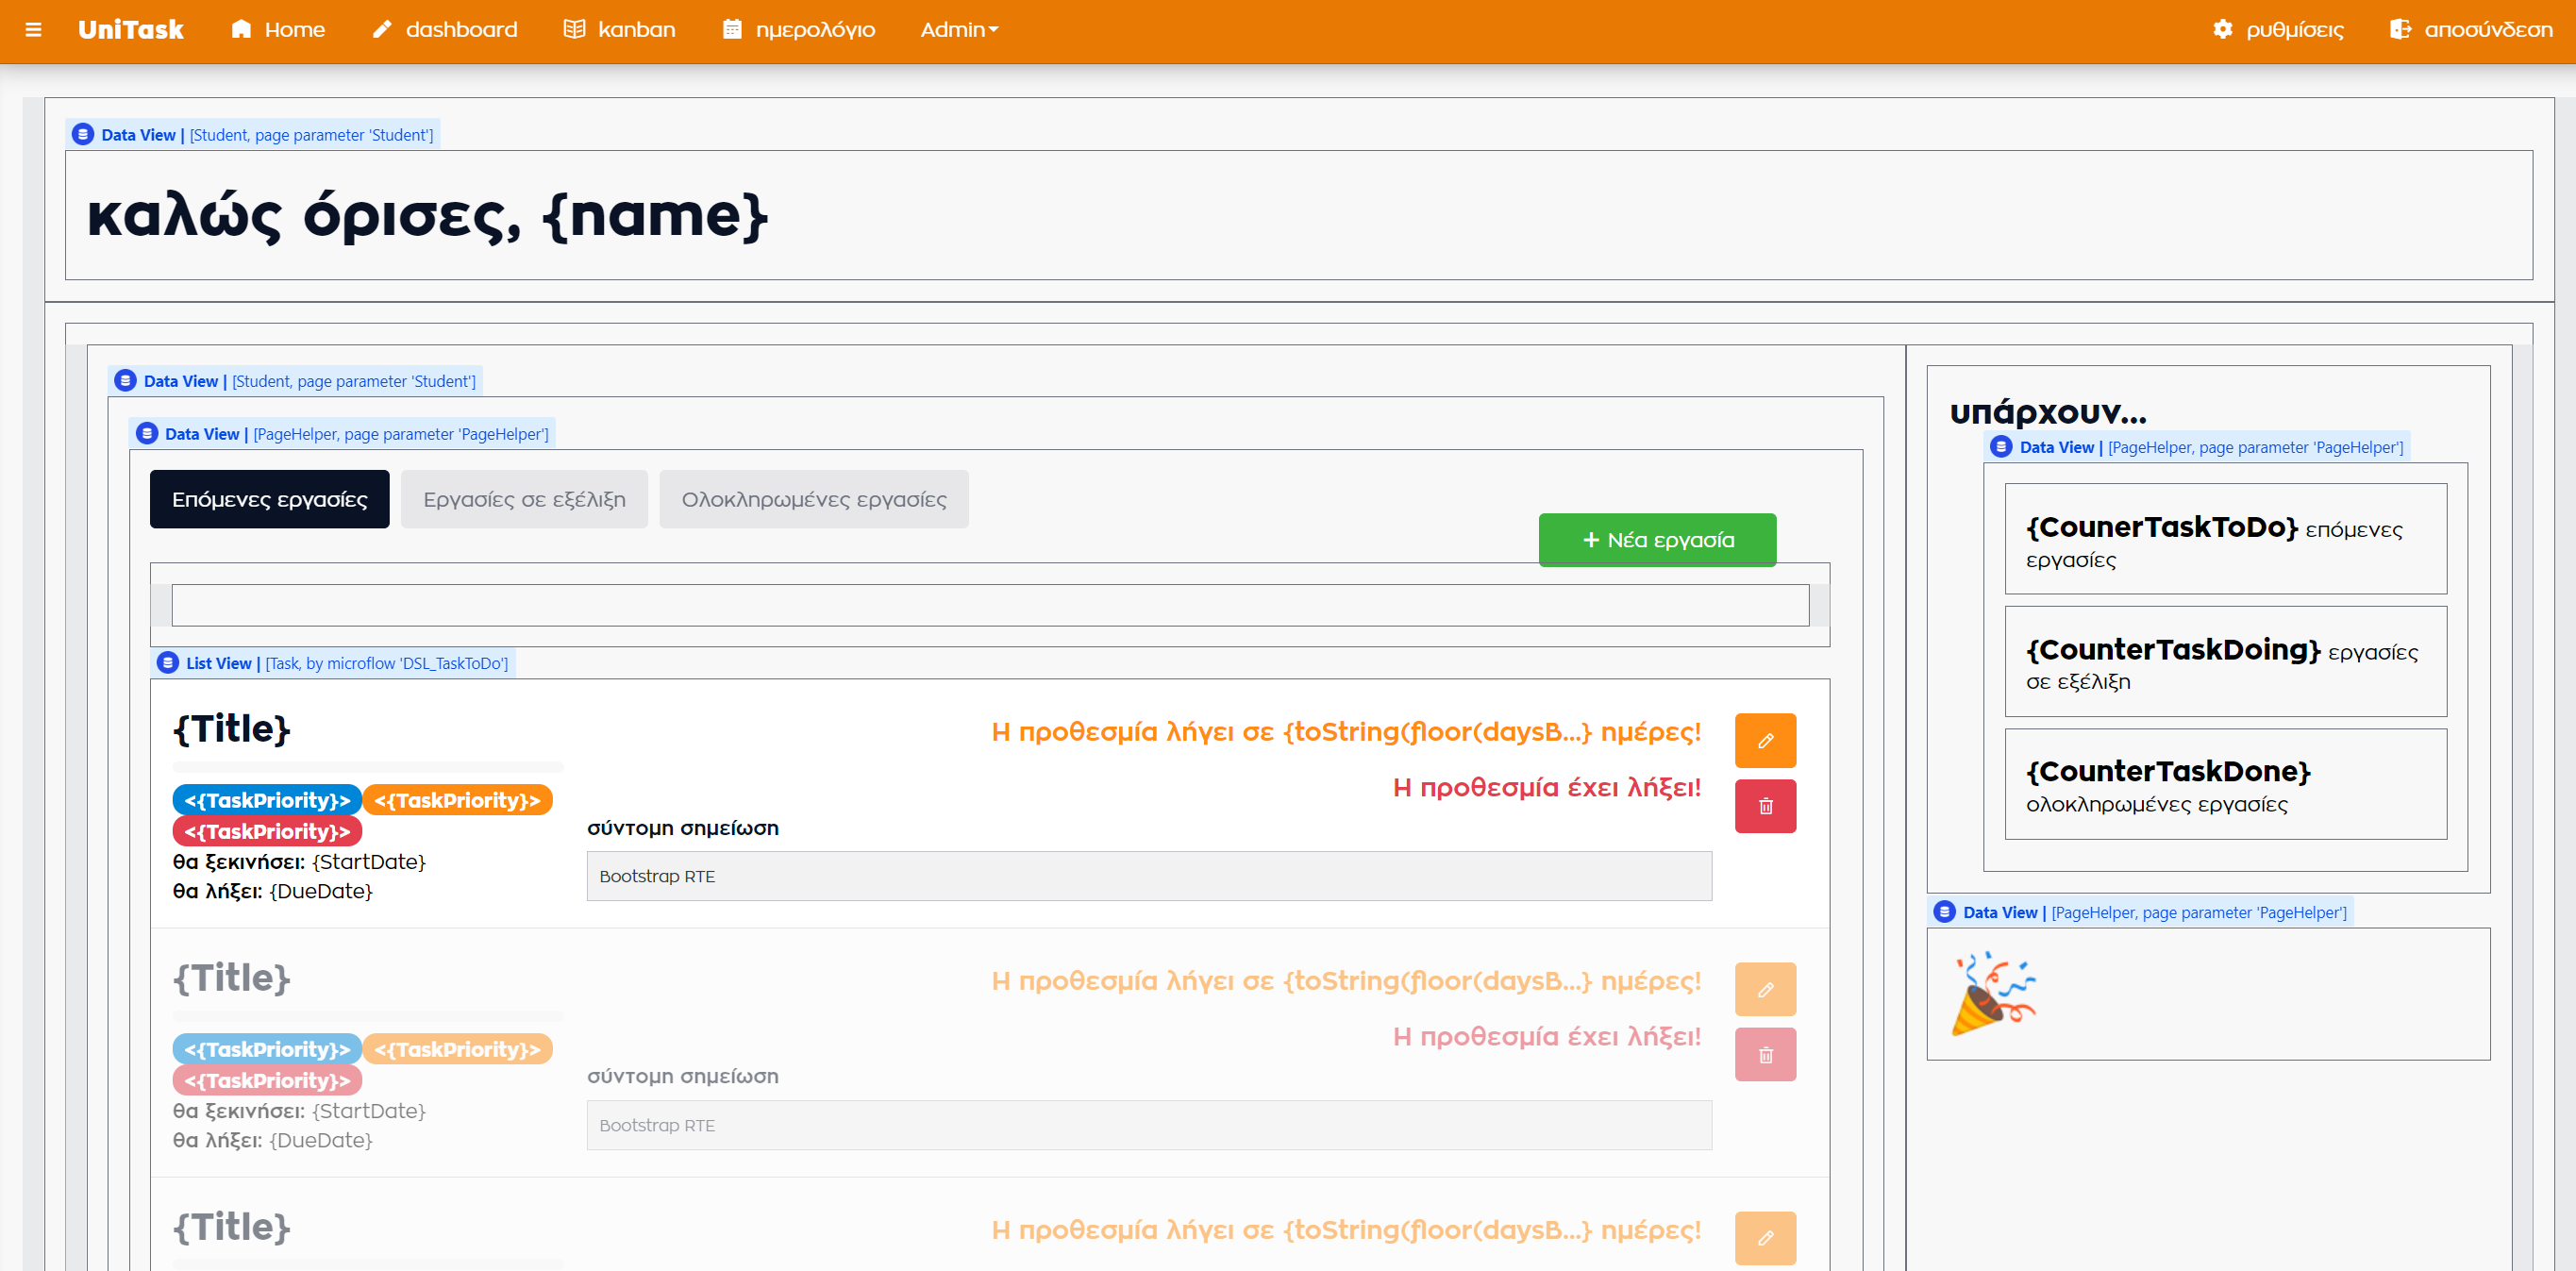
\includegraphics[width=\textwidth]{UniTask_Mendix/PAGE_Tasks_Overview}
                    \end{center}
                \end{figure}

                Η σελίδα χρησιμοποιείται για την εμφάνιση και διαχείριση των εργασιών του χρήστη. Χρησιμοποιεί το \texttt{UniTask\_TopBar} layout του \texttt{UniTaskDesignSystem} module και έχει ως Parameters το \texttt{Student} και το \texttt{PageHelper}.

                Η σελίδα αποτελείται από ένα Layout Grid με διαφορετικά rows. To πρώτο row χρησιμοποιείται για το καλωσόρισμα του χρήστη. Για την εμφάνιση του ονόματός του έχει χρησιμοποιηθεί ένα Data View με Data source το \texttt{Student}. Πίσω από το text widget που εμφανίζει το μήνυμα καλωσορίσματος υπάρχει στην πραγματικότητα η έκφραση \verb|καλώς όρισες, {1}|. Τα \verb|{X}| αποτελούν placeholders για μεταβλητές· στη συγκεκριμένη περίπτωση το \verb|{1}| αντιστοιχεί στο \texttt{Name} του \texttt{Student}.

                Το δεύτερο row του Layout Grid περιλαμβάνει ένα εσωτερικό Layout Grid που δημιουργεί δύο στήλες (9 και 3)\footnote{Χρησιμοποιώντας παρόμοια λογική όπως το Bootstrap, το Mendix χρησιμοποιεί ένα σύστημα 12 στηλών ώστε να καθορίσουμε το πλάτος των στηλών.}. Στην αριστερή στήλη περιλαμβάνονται οι κάρτες με τις εργασίες. Για να επιτευχθεί αυτό έχουν δημιουργηθεί δύο εμφωλευμένα Data Views με Data sources τα \texttt{Student} και \texttt{PageHelper}. Μέσα στο Data View περιλαμβάνεται ένα Tab Container με τρία tabs που αντιστοιχούν στις τρεις καταστάσεις των εργασιών. Σε κάθε tab αντιστοιχίζεται ένα ξεχωριστό πράσινο κουμπί ({\Zona Νέα εργασία}) που, ανάλογα με το tab που είναι ενεργό, καλεί το microflow \texttt{CreateNewTask\_ToDo}, \texttt{CreateNewTask\_Doing} ή \texttt{CreateNewTask\_Done}. Το περιεχόμενο της καρτέλας είναι ένα List View με τις κάρτες εργασιών. Το περιεχόμενο των καρτών γίνεται populate (έχει δηλαδή Data source) από το microflow \texttt{DSL\_TaskToDo}, \texttt{DSL\_TaskDoing} ή \texttt{DSL\_TaskDone} αντίστοιχα. Για την καλύτερη οργάνωση, η κάρτα ουσιαστικά αποτελεί ένα Snippet που επαναχρησιμοποιείται. Έχουν δημιουργηθεί τα Snippets \texttt{TaskCard\_Overview\_Doing}, \texttt{TaskCard\_Overview\_ToDo} και \texttt{TaskCard\_Overview\_Done} που θα αναλυθούν στη συνέχεια.

                Η δεξιά στήλη με τους μετρητές περιλαμβάνει ένα Data View με Data source το \texttt{PageHelper}. Εσωτερικά περιλαμβάνονται containers με text widgets με τις μεταβλητές \texttt{CounterTaskToDo}, \texttt{CounterTaskDoing} και \texttt{CounterTaskDone}.

                Όσον αφορά για το σύστημα επιβράβευσης, το κομφετί αποτελεί ένα add-on widget από το Marketplace του Mendix. Το widget αυτό βρίσκεται τοποθετημένο μέσα σε ένα Data View με Data source το \texttt{PageHelper} και εμφανίζεται μόνο όταν η μεταβλητή \texttt{Confetti} γίνεται \texttt{True}.

                Στο κάτω μέρος του Tab container υπάρχει ένα επεξηγηματικό μπλε παράθυρο (βλέπε σχήμα \ref{fig:unitask_TaskDashboard}) που εμφανίζεται μόνο όταν δεν έχουν δημιουργηθεί εργασίες. Αυτό επιτυγχάνεται με την έκφραση \verb|not($PageHelper/AreThereTasks)| στην συνθήκη Visibility του container που αντιπροσωπεύει το παράθυρο. Αξίζει επίσης να σημειωθεί πως τα call-to-action κουμπιά για τη νέα εργασία και τη σελίδα Kanban είναι και αυτά clickable και έχουν χρησιμοποιηθεί custom CSS κλάσεις για την εμφάνισή τους.

                \begin{figure}[H] \noindent
                    \paragraph{\texttt{TaskCard\_Overview\_Doing}}
                    \begin{center}
                        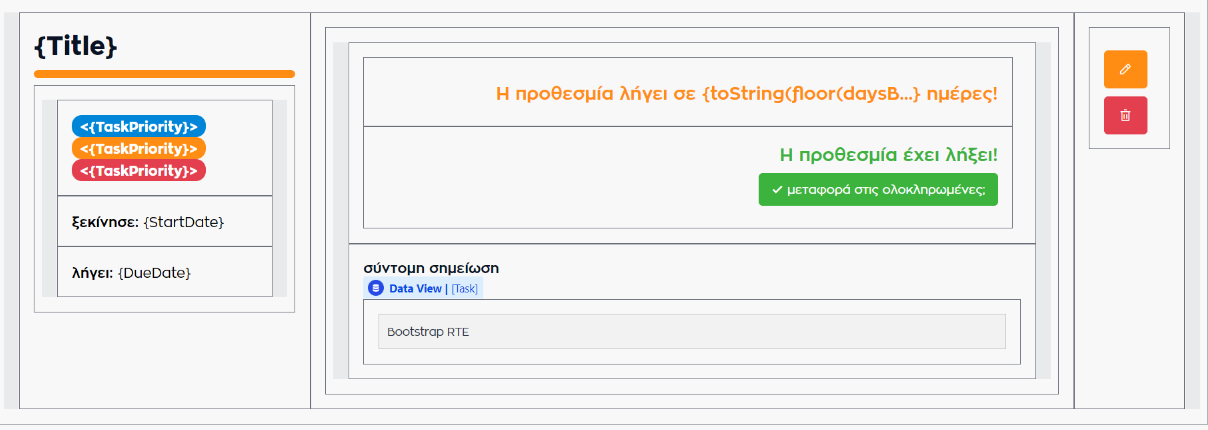
\includegraphics[width=\textwidth]{UniTask_Mendix/TaskCard_Overview_Doing}
                    \end{center}
                \end{figure}

                Πρόκειται για ένα Snippet που χρησιμοποιείται για την εμφάνιση των καρτών με τις εργασίες που βρίσκονται στην κατάσταση \texttt{Doing}. Έχει ως Parameters τα \texttt{Task}, \texttt{PageHelper} και \texttt{Student}.

                Αποτελείται από ένα Layout Grid με τρεις στήλες. Η πρώτη στήλη περιλαμβάνει τον τίτλο, το Progress Bar widget και ένα εσωτερικό Layout Grid με την προτεραιότητα της εργασίας και τις ημερομηνίες έναρξης και λήξης.

                Το Progress Bar χρησιμοποιείται για την εμφάνιση της προόδου της εργασίας και ολοκληρώνεται όσο πλησιάζει η ημερομηνία λήξης. Αυτό επιτυγχάνεται με τον καθορισμό τριών τιμών: Current, Minimum και Maximum value. Στις τιμές Minimum και Maximum value καθορίζονται οι εκφράσεις \verb|dateTimeToEpoch($Task/StartDate)| και \verb|dateTimeToEpoch($Task/DueDate)| αντίστοιχα, στις οποίες ουσιαστικά μετατρέπεται η ημερομηνία και ώρα σε ακέραιο αριθμό. Αυτό βοηθάει στο να είναι καθορισμένο ένα άνω και κάτω αριθμητικό όριο στο οποίο θα κινείται το Current value. Το Current value καθορίζεται από την έκφραση\footnote{Η έκφραση επιστρέφει την τρέχουσα ημερομηνία σε Epoch μορφή, ή --σε περίπτωση που βρισκόμαστε πριν την ημερομηνία έναρξης ή μετά την ημερομηνία λήξης-- αυτές τις ημερομηνίες πάλι σε Epoch μορφή. Η αναπαράσταση μιας χρονικής στιγμής σε Epoch βοηθάει στη σύγκριση μεταξύ ακεραίων για το Progress Bar. Να σημειωθεί πως λέγοντας Epoch μορφή εννοούμε τα δευτερόλεπτα που έχουν περάσει από τη 1η Ιανουαρίου 1970 μέχρι τη χρονική στιγμή που καθορίζουμε.}:

                \begin{lstlisting}[mystyle]
if [%CurrentDateTime%] > $Task/DueDate then dateTimeToEpoch($Task/DueDate)
else if [%CurrentDateTime%] < $Task/StartDate then dateTimeToEpoch($Task/StartDate)
else dateTimeToEpoch([%CurrentDateTime%]) \end{lstlisting}

                \noindent η οποία καταφέρνει τη συγκράτηση της τιμής μέσα σε αυτά τα όρια.

                Η προτεραιότητα εμφανίζεται ως ένα Badge widget. Στην κάρτα βρίσκονται τοποθετημένα και τα τρία, και ανάλογα με το ποιο είναι το \texttt{TaskPriority} εμφανίζεται και εξαφανίζονται τα αντίστοιχα Badges. Τέλος, η ημερομηνία έναρξης και λήξης έχει επιλεχθεί να εμφανίζεται με τη μορφή \texttt{dd MMM yy, h:mm a}, που αντιστοιχεί σε \say{23 Απρ 18, 1:37 μ.μ.} για παράδειγμα.

                Η δεύτερη στήλη περιλαμβάνει ένα Layout Grid με διαφορετικά rows, το πρώτο αφορά δύο containers που εμφανίζονται υπό συνθήκη και περιλαμβάνουν ενημερώσεις για το αν λήγει μια εργασία σε λιγότερο από μια εβδομάδα ή αν έχει ήδη λήξει. Το πρώτο container εμφανίζεται από την έκφραση\footnote{Η έκφραση συγκρίνει τις ημέρες μεταξύ στην τρέχουσα μέρα και της ημερομηνίας λήξης της εργασίας, και επιστέφει \texttt{True} όταν η διαφορά είναι μικρότερη από μια εβδομάδα και η ημερομηνία λήξης ακόμη είναι στο μέλλον.}:
                \begin{lstlisting}[mystyle]
if daysBetween($Task/DueDate, [%CurrentDateTime%]) < 7 and daysBetween($Task/DueDate, [%CurrentDateTime%]) > 0 and $Task/DueDate > [%CurrentDateTime%]
then true else false \end{lstlisting}

                \noindent και εμφανίζει \say{Η προθεσμία λήγει σε \{1\} ημέρες!} όπου το \{1\} αντιστοιχεί σε:

                \begin{lstlisting}[mystyle]
toString(floor(daysBetween($Task/DueDate, [%CurrentDateTime%]))) \end{lstlisting}

                To δεύτερο container εμφανίζεται το \verb|[%CurrentDateTime]| είναι μικρότερο ή ίσο από το \texttt{DueDate} και το κουμπί του καλεί το microflow \texttt{ChangeTaskStatus\_TaskDone}.

                Κάτω από το container υπάρχει ένα Data View με Data source το \texttt{Task} και το Bootstrap RTE widget. Το Rich Text Editor παρέχει στους χρήστες τη δυνατότητα δημιουργίας εμπλουτισμένου περιεχομένου, όπως έντονο (bold) και πλάγιο (italic) κείμενο. Το widget αποθηκεύει το κείμενο σε String μορφή.

                Στη δεξιά στήλη υπάρχουν τα κουμπιά επεξεργασίας και διαγραφής που καλούν τα microflows \texttt{EditTask} και \texttt{DeleteTask} (μετά από επιβεβαίωση) αντίστοιχα. Να σημειωθεί πως το κουμπί διαγραφής εμφανίζεται ανάλογα με την τιμή της Boolean ιδιότητας \texttt{buttonQuickDelete} του \texttt{Student}.

                \begin{figure}[H] \noindent
                    \paragraph{\texttt{TaskCard\_Overview\_ToDo}}
                    \begin{center}
                        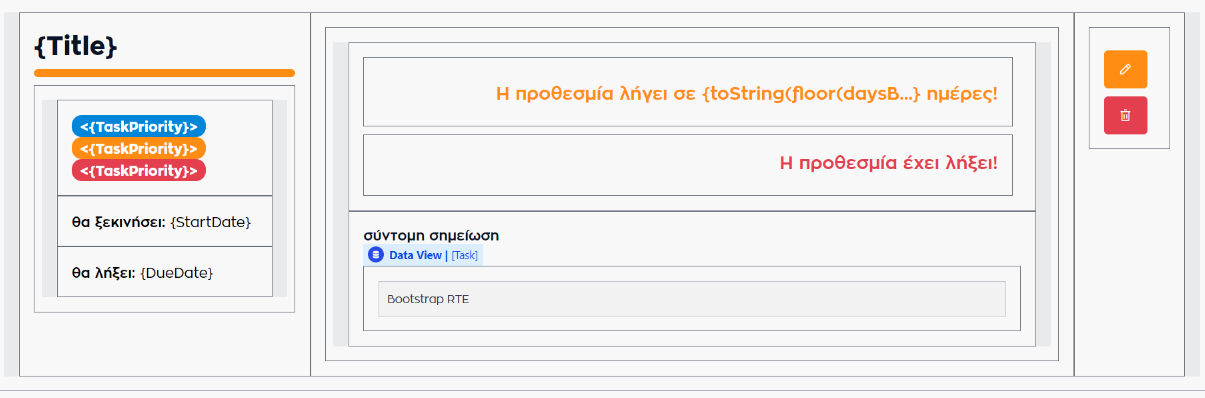
\includegraphics[width=\textwidth]{UniTask_Mendix/TaskCard_Overview_ToDo}
                    \end{center}

                    \paragraph{\texttt{TaskCard\_Overview\_Done}}
                    \begin{center}
                        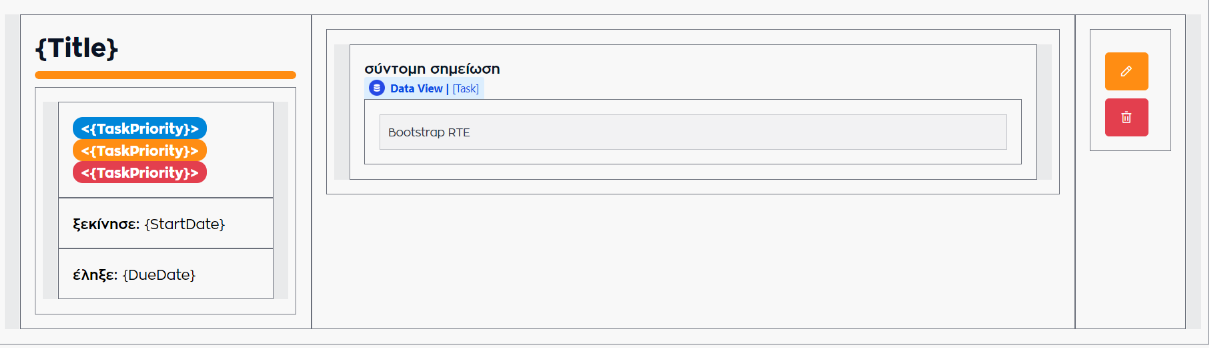
\includegraphics[width=\textwidth]{UniTask_Mendix/TaskCard_Overview_Done}
                    \end{center}
                \end{figure}

                Τα Snippets \texttt{TaskCard\_Overview\_ToDo} και \texttt{TaskCard\_Overview\_Done} είναι παρόμοια με το \texttt{TaskCard\_Overview\_Doing} με τις απαραίτητες διαφοροποιήσεις.

                Να σημειωθεί πως στο \texttt{TaskCard\_Overview\_Done} το Progress Bar πάντα είναι ολοκληρωμένο, ενώ το \texttt{TaskCard\_Overview\_ToDo} πάντα κενό, και επίσης πως στο δεύτερο δεν υπάρχει call-to-action κουμπί για την αλλαγή κατάστασης της εργασίας μετά την ημερομηνία λήξης, καθώς σε ένα σενάριο που ο χρήστης έχει προσθέσει μια εργασία ως To-Do και έχει τελειώσει η προθεσμία της πριν περάσει στην Doing κατάσταση, η προβλεπόμενη κίνηση θα είναι να τη διαγράψει.

                \begin{figure}[H] \noindent
                    \paragraph{\texttt{POPOUT\_Task\_NewEdit}}
                    \begin{center}
                        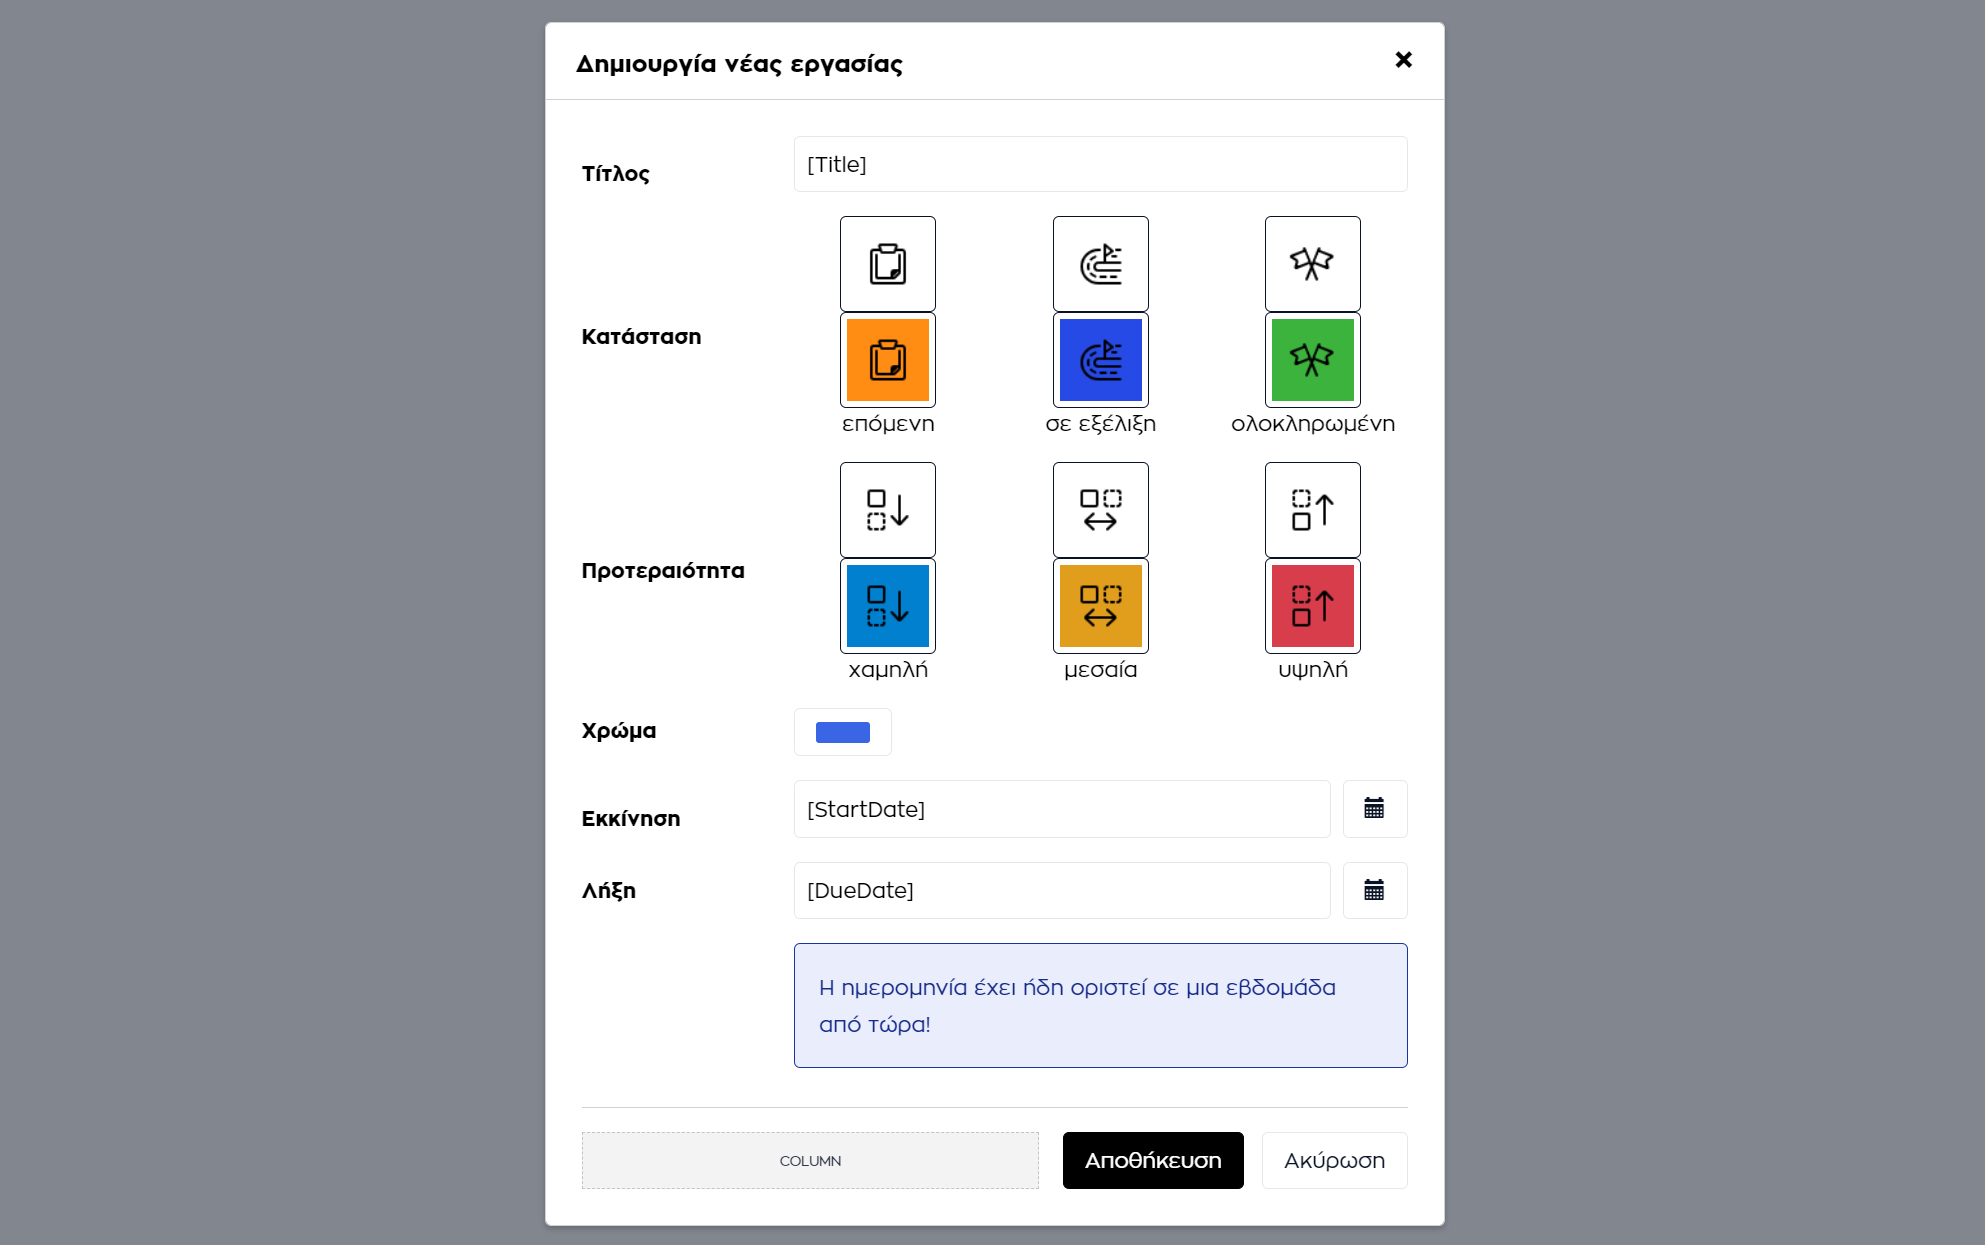
\includegraphics[width=\textwidth]{UniTask_Mendix/POPOUT_Task_NewEdit}
                    \end{center}
                \end{figure}

                Η σελίδα καλείται στα microflows \texttt{CreateNewTask\_ToDo}, \texttt{CreateNewTask\_Doing} και \texttt{CreateNewTask\_Done} και χρησιμοποιείται για τη δημιουργία νέων εργασιών. Χρησιμοποιεί το \texttt{Popout\_Layout} layout του \texttt{Atlas\_Core} και έχει ως Parameters το \texttt{Task} και το \texttt{PageHelper}.

                Περιλαμβάνει ένα Data View με ένα Layout Grid με τα απαραίτητα Text Boxes και Date Pickers για την εισαγωγή του τίτλου και των ημερομηνιών έναρξης και λήξης. Για την επιλογή του χρώματος χρησιμοποιείται το widget ColorPicker που αποθηκεύει το επιλεγμένο χρώμα στη μεταβλητή \texttt{CalendarColor}.

                Για την επιλογή της κατάστασης και της προτεραιότητας έχουν δημιουργηθεί ένα σύνολο από ζεύγη κουμπιών, το ένα άχρωμο και το άλλο έγχρωμο. Ανάλογα με το ποιο είναι το \texttt{TaskStatus} και το \texttt{TaskPriority} εμφανίζεται και εξαφανίζεται το αντίστοιχο σύνολο κουμπιών. Ταυτόχρονα, οι λεζάντες κάτω από τα κουμπιά περιέχουν τη δυναμική κλάση που καθορίζεται από την έκφραση:

                \begin{lstlisting}[mystyle]
if $Task/TaskPriority = TaskManager.TaskPriority.Low then 'labelSelected'
else ''         \end{lstlisting}

Αντίστοιχα στο αρχείο \verb|Styling/web/custom-variables.scss| έχει δημιουργηθεί η κλάση:
                \begin{lstlisting}[mystyle]
.labelSelected {
    font-weight: bold;
}                \end{lstlisting}

                Με αυτόν τον τρόπο επιτυγχάνεται η εμφάνιση της επιλεγμένης κατάστασης και προτεραιότητας με έντονη γραφή. Επιπλέον, το κάθε σύνολο από τα ζεύγη κουμπιών βρίσκεται τοποθετημένο σε ένα container, το οποίο αν πατηθεί καλεί τα microflow \texttt{ChangeTaskStatus\_TaskToDo}, \texttt{ChangeTaskStatus\_TaskDoing}, \texttt{ChangeTaskStatus\_}\linebreak\texttt{TaskDone} και \texttt{ChangeTaskPriority\_Low}, \texttt{ChangeTaskPriority\_Medium} και \linebreak \texttt{ChangeTaskPriority\_High} αντίστοιχα.

                Τέλος, η εμφάνιση του μπλε παραθύρου που ενημερώνει ότι η ημερομηνία λήξης έχει προκαθοριστεί αυτόματα βασίζεται στην Boolean μεταβλητή \texttt{CreationDateBubble} του \texttt{Task}, και επίσης όταν γίνεται κλικ στο Date Picker για την ημερομηνία λήξης, καλείται το microflow  \texttt{DisableCreationDateBubble}.

                Για να αποθηκευτεί η νέα εργασία καλείται το microflow \texttt{SaveTask}.

                \begin{figure}[H] \noindent
                    \paragraph{\texttt{POPOUT\_Task\_NewEdit\_Edit}}
                    \begin{center}
                        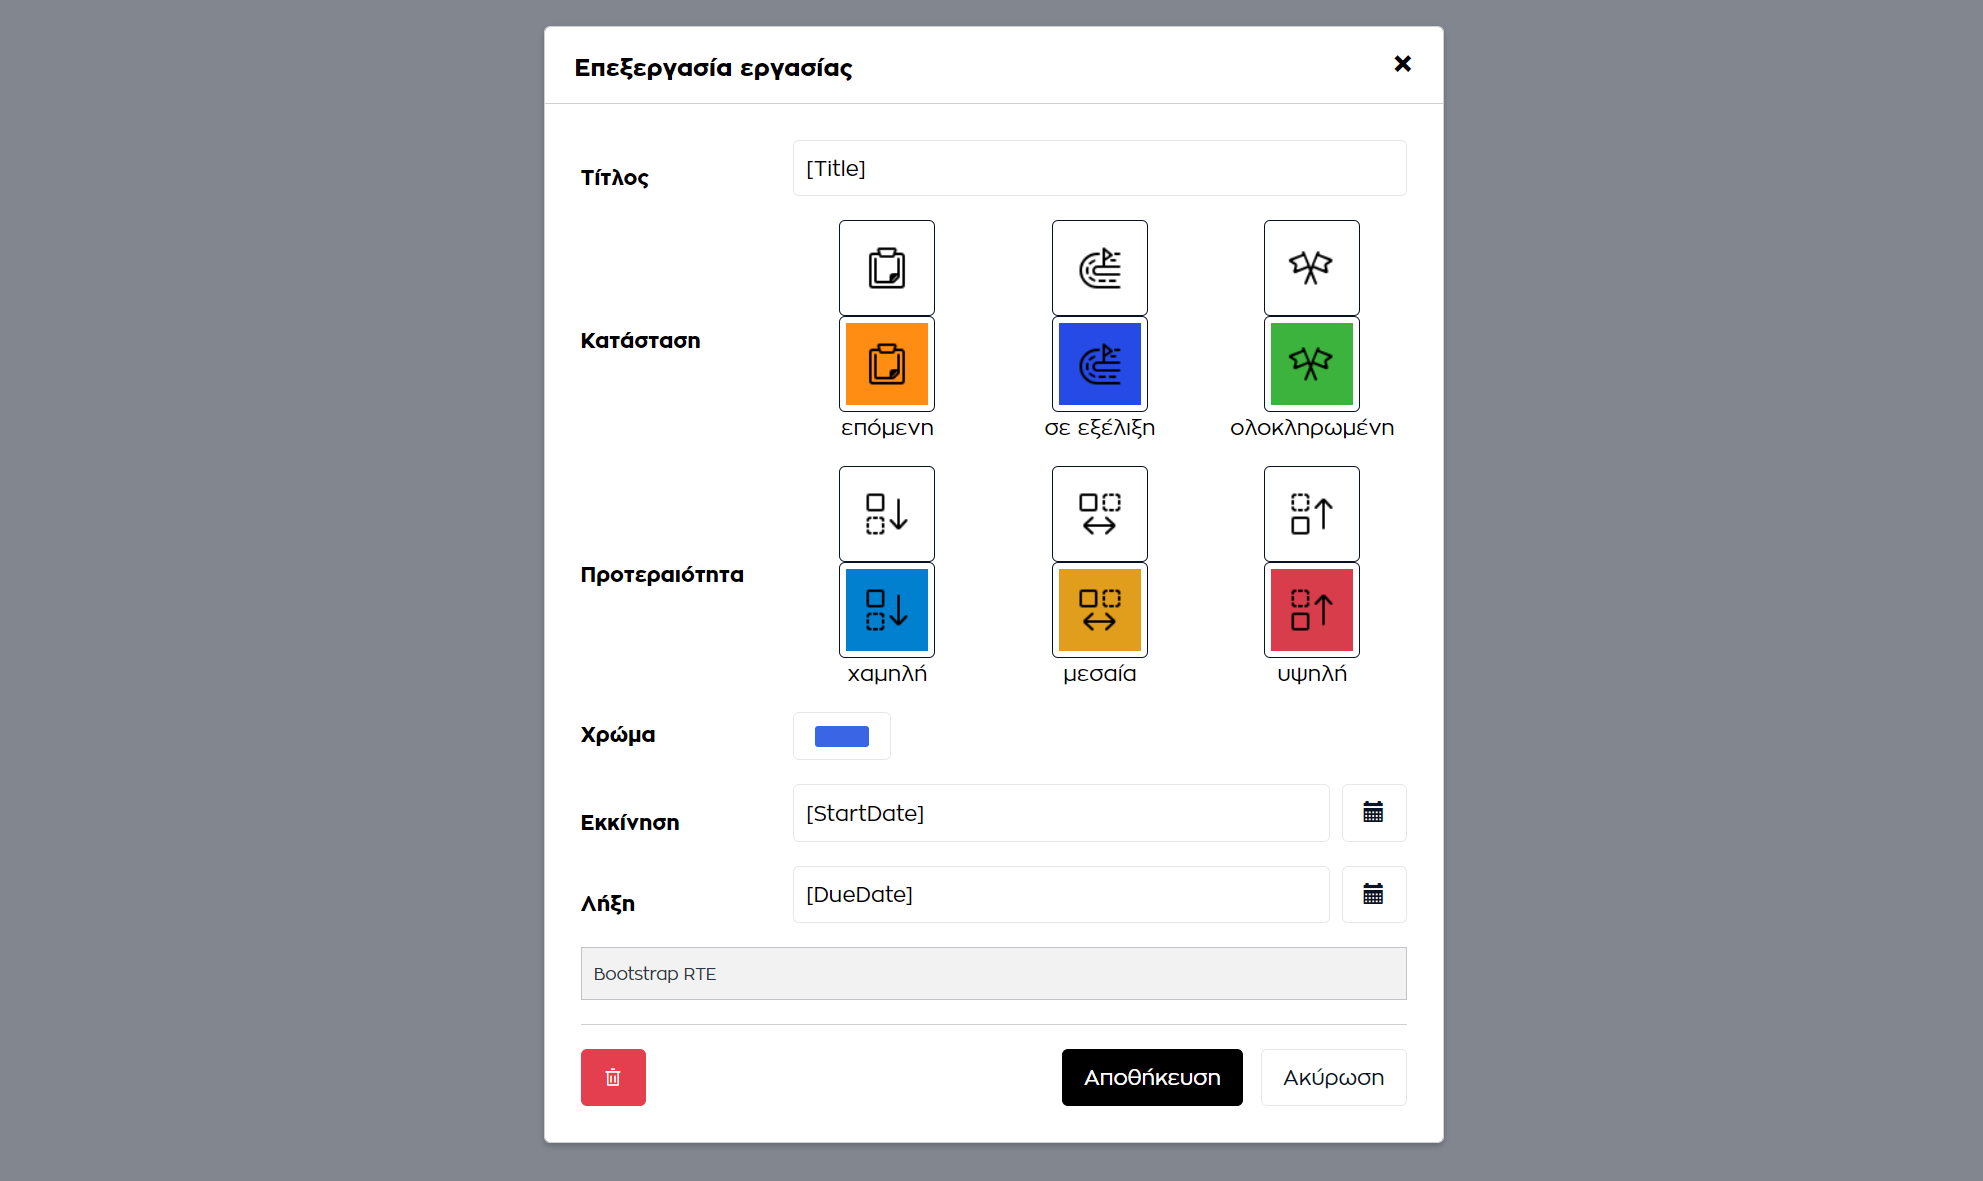
\includegraphics[width=\textwidth]{UniTask_Mendix/POPOUT_Task_NewEdit_Edit}
                    \end{center}
                \end{figure}

                Η σελίδα καλείται από το microflow \texttt{Edit\_Task}. Χρησιμοποιείται αντίστοιχη λογική με την \texttt{POPOUT\_Task\_NewEdit} με τη διαφορά ότι δεν υπάρχει επεξηγηματικό παράθυρο για την ημερομηνία λήξης, υπάρχει το widget Bootstrap RTE για την επεξεργασία της ιδιότητας \texttt{Notes} και επιπλέον υπάρχει το κουμπί διαγραφής της εργασίας που καλεί το microflow \texttt{DeleteTask} μετά από επιβεβαίωση.

                \begin{figure}[H] \noindent
                    \paragraph{\texttt{PAGE\_Tasks\_Kanban}}
                    \begin{center}
                        \includegraphics[width=\textwidth]{UniTask_Mendix/PAGE_Tasks_Kanban}
                    \end{center}
                \end{figure}

                Η σελίδα χρησιμοποιείται ως ένας εναλλακτικός τρόπος εμφάνισης των εργασιών του χρήστη σε έναν Kanban πίνακα. Χρησιμοποιεί το \texttt{UniTask\_TopBar} layout του \texttt{UniTaskDesignSystem} module και έχει ως Parameter το \texttt{PageHelper}.

                Η σελίδα αποτελείται από ένα Layout Grid με 3 στήλες, με τις δύο ακραίες να αποτελούν negative space. Η κεντρική στήλη περιέχει ένα Layout Grid με 3 στήλες. Το πρώτο row του περιλαμβάνει τις επικεφαλίδες του πίνακα μαζί με κουμπιά για την προσθήκη νέας εργασίας. Κάθε κουμπί είναι προσαρμοσμένο να δημιουργεί μια εργασία που αντιστοιχεί στην κατάσταση της επικεφαλίδας, καλώντας τα microflows \texttt{CreateNewTask\_ToDo}, \texttt{CreateNewTask\_Doing} και \texttt{CreateNewTask\_Done} αντίστοιχα. Το δεύτερο row περιλαμβάνει Galleries με Data sources τα \texttt{DSL\_TaskToDo}, \texttt{DSL\_TaskDoing} και \texttt{DSL\_TaskDone} που δημιουργούν τις κάρτες, που αν πατηθούν καλούν το microflow \texttt{EditTask}. Τέλος, περιλαμβάνεται το Confetti widget, όπως και στην Dashboard σελίδα.

                \begin{figure}[H] \noindent
                    \paragraph{\texttt{TaskCard\_Kanban}}
                    \begin{center}
                        \includegraphics[width=\textwidth]{UniTask_Mendix/TaskCard_Kanban}
                    \end{center}
                \end{figure}

                Πρόκειται για ένα Snippet που χρησιμοποιείται για την εμφάνιση των καρτών με τις εργασίες στον πίνακα Kanban. Έχει ως Parameters τα \texttt{Task} και \texttt{Student}.

                Αποτελείται από ένα Layout Grid με τον τίτλο, τις ημερομηνίες έναρξης και λήξης και Badges για την προτεραιότητα της εργασίας, με παρόμοιο τρόπο όπως στα Snippets του Dashboard.

                \begin{figure}[H] \noindent
                    \paragraph{\texttt{PAGE\_Calendar}}
                    \begin{center}
                        \includegraphics[width=\textwidth]{UniTask_Mendix/PAGE_Calendar}
                    \end{center}
                \end{figure}

                Η σελίδα χρησιμοποιείται για την εμφάνιση των εργασιών του χρήστη σε έναν ημερολόγιο. Χρησιμοποιεί το \texttt{UniTask\_TopBar} layout του \texttt{UniTaskDesignSystem} module και έχει ως Parameter το \texttt{Task} και \texttt{PageHelper}.

                Το Calendar widget είναι τοποθετημένο μέσα σε ένα Data View με Data source το \texttt{Task}. Έτσι καθορίζεται πως το Event entity, δηλαδή ο τύπος αντικειμένου που θα εμφανίζεται στο ημερολόγιο, είναι το \texttt{Task}. Το ημερολόγιο γίνεται populate μέσω του microflow \texttt{ShowTasks\_Calendar} και στα Properties του Widget επιλέγονται οι ιδιότητες \texttt{Title}, \texttt{StartDate}, \texttt{DueDate} και \texttt{CalendarColor} του \texttt{Task} για να καθοριστεί η εμφάνισή του στο ημερολόγιο. Όσον αφορά το Timeline στα δεξιά του, έχει επιλεχθεί να εμφανίζονται οι εργασίες ομαδοποιημένες βάσει της ημερομηνίας έναρξής τους και μάλιστα να μπορεί να γίνει επεξεργασία τους αν γίνει κλικ πάνω τους.

                \begin{figure}[H] \noindent
                    \paragraph{\texttt{PAGE\_Settings}}
                    \begin{center}
                        \includegraphics[width=\textwidth]{UniTask_Mendix/PAGE_Settings}
                    \end{center}
                \end{figure}

                Η σελίδα χρησιμοποιείται για την εμφάνιση των ρυθμίσεων του χρήστη. Χρησιμοποιεί το \texttt{UniTask\_TopBar} layout του \texttt{UniTaskDesignSystem} module και έχει ως Parameters το \texttt{Student} και το \texttt{PageHelper}.

                Οι ρυθμίσεις βρίσκονται τοποθετημένες σε ένα Accordion widget με δύο ομάδες: διαγραφή και αρχικοποίηση. Στη διαγραφή περιλαμβάνεται ένα Data View με Data source το \texttt{Student}. Εσωτερικά του υπάρχει ένα Switch widget που κάνει toggle την Boolean ιδιότητα \texttt{buttonQuickDelete} του \texttt{Student} και ένα κουμπί ({\Zona διαγραφή όλων των εργασιών}) που καλεί το microflow \texttt{DeleteAllTasks} μετά από επιβεβαίωση. Στην αρχικοποίηση περιλαμβάνεται το κουμπί ({\Zona αρχικοποίηση}) που καλεί το microflow \texttt{InitializeTasks} μετά από επιβεβαίωση.

            \subsubsection{Microflows του \texttt{TaskManager}}
                Στο \texttt{TaskManager} περιλαμβάνονται τα εξής microflows\footnote{Στα ονόματα των microflows περιλαμβάνεται ο parent φάκελος όπου βρίσκονται για τον πιο εμφανή διαχωρισμό τους.}:

                \begin{figure}[H] \noindent
                    \paragraph{\texttt{RET\_Student}}
                    \begin{center}
                        \includegraphics[width=\textwidth]{UniTask_Mendix/RET_Student}
                    \end{center}
                \end{figure}

                Το microflow χρησιμοποιείται για την ανάκτηση του \texttt{Student} με βάση τον τρέχοντα \texttt{System.User}. Αν δεν υπάρχει τέτοιος χρήστης, τότε το microflow επιστρέφει ένα κενό αντικείμενο, αλλιώς επιστρέφεται το \texttt{Student}.

                \begin{figure}[H] \noindent
                    \paragraph{\texttt{Auxiliary/AreThereTasks}}
                    \begin{center}
                        \includegraphics[width=\textwidth]{UniTask_Mendix/AreThereTasks}
                    \end{center}
                \end{figure}

                To microflow χρησιμοποιείται από το domain model για τον υπολογισμό της τιμής της Boolean ιδιότητας \texttt{AreThereTasks} του \texttt{PageHelper}.

                Το microflow καλεί το microflow \texttt{CounterTotalTasks}, το οποίο επιστρέφει ως Integer τον συνολικό αριθμό των εργασιών του χρήστη. Αν ο αριθμός είναι μεγαλύτερος ή ίσος του 1, τότε το microflow επιστρέφει \texttt{true}, αλλιώς \texttt{false}.

                \begin{figure}[H] \noindent
                    \paragraph{\texttt{Auxiliary/DisableCreationDateBubble}}
                    \begin{center}
                        \includegraphics[width=\textwidth]{UniTask_Mendix/DisableCreationDateBubble}
                    \end{center}
                \end{figure}

                Το microflow χρησιμοποιείται από τη σελίδα \texttt{POPOUT\_Task\_NewEdit} για να απενεργοποιήσει το μπλε παράθυρο που ενημερώνει ότι η ημερομηνία λήξης έχει προκαθοριστεί αυτόματα. Καλείται όταν ο χρήστης αλλάζει την ημερομηνία λήξης της εργασίας.

                Το microflow αλλάζει την τιμή της Boolean ιδιότητας \texttt{CreationDateBubble} του \texttt{Task} σε \texttt{false}.

                \begin{figure}[H] \noindent
                    \paragraph{\texttt{ChangeTaskPriorities/ChangeTaskPriority\_TaskLow} \\ \texttt{ChangeTaskPriorities/ChangeTaskPriority\_TaskMedium} \\ \texttt{ChangeTaskPriorities/ChangeTaskPriority\_TaskHigh}}
                    \begin{center}
                        \includegraphics[width=\textwidth]{UniTask_Mendix/ChangeTaskPriority}
                    \end{center}
                \end{figure}

                Τα microflows χρησιμοποιούνται για την αλλαγή της προτεραιότητας κάποιας εργασίας. Καλούνται από τα κουμπιά της σελίδας \texttt{POPOUT\_Task\_NewEdit} και \texttt{POPOUT\_Task\_NewEdit\_Edit}.

                Το κάθε microflow αλλάζει την τιμή της Enumeration ιδιότητας \texttt{TaskPriority} του \texttt{Task} σε \texttt{Low}, \texttt{Medium} και \texttt{High} αντίστοιχα.

                \begin{figure}[H] \noindent
                    \paragraph{\texttt{ChangeTaskStatuses/ChangeTaskStatus\_TaskDoing} \\ \texttt{ChangeTaskStatuses/ChangeTaskStatus\_TaskToDo} \\ \texttt{ChangeTaskStatuses/ChangeTaskStatus\_TaskDone}}
                    \begin{center}
                        \includegraphics[width=\textwidth]{UniTask_Mendix/ChangeTaskStatus}
                        \includegraphics[width=\textwidth]{UniTask_Mendix/ChangeTaskStatus_TaskDone}
                    \end{center}
                \end{figure}

                Τα microflows χρησιμοποιούνται για την αλλαγή της κατάστασης κάποιας εργασίας. Καλούνται από τα κουμπιά της σελίδας \texttt{POPOUT\_Task\_NewEdit} και \texttt{POPOUT\_Task\_NewEdit\_Edit}.

                Το κάθε microflow αλλάζει την τιμή της Enumeration ιδιότητας \texttt{TaskStatus} του \texttt{Task} σε \texttt{TaskStatus.Doing}, \texttt{TaskStatus.ToDo} και \texttt{TaskStatus.Done} αντίστοιχα. Επιπλέον, στην περίπτωση του microflow \texttt{ChangeTaskStatus\_TaskDone} καλεί το microflow \texttt{ConfettiTrigger} για το εφέ του κομφετί.

                \begin{figure}[H] \noindent
                    \paragraph{\texttt{Confetti/Confetti}}
                    \begin{center}
                        \includegraphics[width=\textwidth]{UniTask_Mendix/ConfettiTrigger}
                    \end{center}
                \end{figure}

                Το microflow καλείται από το microflow \texttt{ChangeTaskStatus\_TaskDone} και χρησιμοποιείται για την εμφάνιση του εφέ κομφετί στην οθόνη του χρήστη. Αλλάζει την τιμή της Boolean ιδιότητας \texttt{Confetti} του \texttt{PageHelper} σε \texttt{true}.

                \begin{figure}[H] \noindent
                    \paragraph{\texttt{Confetti/Confetti}}
                    \begin{center}
                        \includegraphics[width=\textwidth]{UniTask_Mendix/ConfettiNotTriggering}
                    \end{center}
                \end{figure}

                Το microflow καλείται από το microflow \texttt{SaveTask} και χρησιμοποιείται για να επαναφέρει την τιμή της Boolean ιδιότητας \texttt{Confetti} του \texttt{PageHelper} σε \texttt{false}.

                \begin{figure}[H] \noindent
                    \paragraph{\texttt{ShowTasks/DSL\_TaskDoing} \\ \texttt{ShowTasks/DSL\_TaskDone} \\ \texttt{ShowTasks/DSL\_TaskToDo}}
                    \begin{center}
                        \includegraphics[width=\textwidth]{UniTask_Mendix/DSL_TaskDoingDoneToDo}
                    \end{center}
                \end{figure}

                Τα microflows φιλτράρουν και επιστρέφουν τις εργασίες του χρήστη ανάλογα με την κατάστασή τους. Χρησιμοποιούνται από τις σελίδες \texttt{PAGE\_Tasks\_Overview} και \texttt{PAGE\_Tasks\_Kanban} και τα microflows \texttt{ShowTasks\_Calendar} και \texttt{CounterTaskDoing}.

               Με Parameter το \texttt{Student}, το microflow κάνει retrieve τη λίστα των Tasks (αφού συσχετίζονται). Η λίστα φιλτράρεται βάσει του \texttt{TaskStatus}, ταξινομείται βάσει δύο ιδιοτήτων σε αύξουσα σειρά, τα \texttt{TaskPriority} και \texttt{DueDate}, και επιστρέφεται.

                \begin{figure}[H] \noindent
                    \paragraph{\texttt{ShowTasks/ShowTasks\_Calendar}}
                    \begin{center}
                        \includegraphics[width=\textwidth]{UniTask_Mendix/ShowTasks_Calendar}
                    \end{center}
                \end{figure}

                Το microflow επιστρέφει το σύνολο των εργασιών του χρήστη για την εμφάνισή τους στο ημερολόγιο.

                Το \texttt{RET\_Student} επιστρέφει το \texttt{Student}, ώστε να χρησιμοποιηθεί ως παράμετρος στα microflows \texttt{DSL\_TaskDoing}, \texttt{DSL\_TaskDone} και \texttt{DSL\_TaskToDo}, τα οποία καλούνται και οι λίστες τους επιστρέφονται. Στη συνέχεια με List Operations οι λίστες συνενώνονται, ταξινομούνται βάσει της ημερομηνίας έναρξης και επιστρέφονται.

                Ο λόγος που δε χρησιμοποιείται κάποια παράμετρος \texttt{Student} απευθείας και καλείται η \texttt{RET\_Student} είναι γιατί από τη φύση του Calendar widget είναι απαραίτητο να βρίσκεται σε ένα Data View με Data source το \texttt{Task}, άρα κατά συνέπεια θα έχει παράμετρο το \texttt{Task}.

                \begin{figure}[H] \noindent
                    \paragraph{\texttt{CounterGenerators/CounterTaskDoing} \\ \texttt{CounterGenerators/CounterTaskDone} \\ \texttt{CounterGenerators/CounterTaskToDo}}
                    \begin{center}
                        \includegraphics[width=\textwidth]{UniTask_Mendix/CounterTask}
                    \end{center}
                \end{figure}

                Τα microflows χρησιμοποιούνται για τον υπολογισμό του συνολικού αριθμού των εργασιών του χρήστη ανάλογα με την κατάστασή τους, και καλούνται από το domain model για τον υπολογισμό των τιμών των ιδιοτήτων \texttt{TaskToDoCount}, \texttt{TaskDoingCount} και \texttt{TaskDoneCount} του \texttt{PageHelper}.

                Το κάθε microflow καλεί το \texttt{RET\_Student} και τα microflows \texttt{DSL\_TaskToDo}, \texttt{DSL\_TaskDoing} και \texttt{DSL\_TaskDone} αντίστοιχα. Έπειτα μέσω του Function Count του Aggregate List Action του Mendix, υπολογίζει τον αριθμό των εργασιών και τον επιστρέφει.

                \begin{figure}[H] \noindent
                    \paragraph{\texttt{CounterGenerators/CounterTotalTasks}}
                    \begin{center}
                        \includegraphics[width=\textwidth]{UniTask_Mendix/CounterTotalTasks}
                    \end{center}
                \end{figure}

                Το microflow καλείται από το microflow \texttt{AreThereTasks} και χρησιμοποιείται για τον υπολογισμό του συνολικού αριθμού των εργασιών του χρήστη. Χρησιμοποιείται παρόμοια λογική με τα προηγούμενα microflows: γίνεται retrieve το σύνολο των εργασιών για έναν συγκεκριμένο χρήστη και καταμετρούνται.

                \begin{figure}[H] \noindent
                    \paragraph{\texttt{CreateNewTask/CreateNewTask\_Doing} \\ \texttt{CreateNewTask/CreateNewTask\_Done} \\ \texttt{CreateNewTask/CreateNewTask\_ToDo}}
                    \begin{center}
                        \includegraphics[width=\textwidth]{UniTask_Mendix/CreateNewTask}
                    \end{center}
                \end{figure}

                To microflow καλείται από τα κουμπιά {\Zona νέα εργασία} των σελίδων \texttt{PAGE\_Tasks\_Kanban} και \texttt{PAGE\_Tasks\_Overview} με σκοπό τη δημιουργία μιας νέας εργασίας.

                Αρχικά καλείται το microflow \texttt{RET\_Student} για την ανάκτηση του \texttt{Student}. Στη συνέχεια δημιουργείται ένα νέο αντικείμενο τύπου \texttt{Task} όπου ορίζονται κάποιες αρχικές τιμές. Συγκεκριμένα ορίζεται η ημερομηνία λήξης \texttt{DueDate} ως \linebreak \verb|addDays([%CurrentDateTime%], 7)| (μια εβδομάδα μετά την τρέχουσα ημερομηνία), ο τίτλος \texttt{Title} ως \texttt{'Νέα εργασία'}, και το \texttt{TaskStatus} ανάλογα με το τύπο του microflow. Έπειτα, εμφανίζεται η αναδυόμενη σελίδα \texttt{POPOUT\_Task\_NewEdit} για την επεξεργασία των ιδιοτήτων της εργασίας και την τελική αποθήκευσή της.

                \begin{figure}[H] \noindent
                    \paragraph{\texttt{ShowPages/ShowPage\_Calendar} \\ \texttt{ShowPages/ShowPage\_Homepage} \\ \texttt{ShowPages/ShowPage\_Kanban} \\ \texttt{ShowPages/ShowPage\_Settings} \\ \texttt{ShowPages/ShowPage\_TasksOverview}}
                    \begin{center}
                        \includegraphics[width=\textwidth]{UniTask_Mendix/ShowPage}
                    \end{center}
                \end{figure}

                Τα microflows χρησιμοποιούνται για την ανακατεύθυνση του χρήστη σε μια συγκεκριμένη σελίδα. Καλούνται όποτε χρειάζεται η εμφάνιση μιας σελίδας, κυρίως από το Navigation μενού.

                Αφού ανακτηθεί το \texttt{Student} μέσω του microflow \texttt{RET\_Student}, το εκάστοτε microflow δημιουργεί ένα \texttt{PageHelper} αντικείμενο και εμφανίζει την αντίστοιχη σελίδα. Η δημιουργία του \texttt{PageHelper} είναι απαραίτητη καθώς χρησιμοποιείται ως Parameter στις σελίδες.

                \begin{figure}[H] \noindent
                    \paragraph{\texttt{SaveTask}}
                    \begin{center}
                        \includegraphics[width=\textwidth]{UniTask_Mendix/SaveTask}
                    \end{center}
                \end{figure}

                Το microflow καλείται από τις αναδυόμενες σελίδες \texttt{POPOUT\_Task\_NewEdit} και \texttt{POPOUT\_Task\_NewEdit\_Edit} για την αποθήκευση των αλλαγών που έγιναν στις ιδιότητες της εργασίας.

                Γίνεται commit στο αντικείμενο \texttt{Task}, κλείνει η σελίδα, γίνεται ένα Change Object στο \texttt{PageHelper} για να ανανεωθούν οι τιμές του, όπως υπολογίζονται από τα microflows και καλείται το microflow \texttt{ConfettiNotTriggering} για την επαναφορά της τιμής της Boolean ιδιότητας \texttt{Confetti} του \texttt{PageHelper} σε \texttt{false}.

                \begin{figure}[H] \noindent
                    \paragraph{\texttt{EditTask}}
                    \begin{center}
                        \includegraphics[width=\textwidth]{UniTask_Mendix/EditTask}
                    \end{center}
                \end{figure}

                Το microflow καλείται από τα κουμπιά των καρτών στην Dashboard σελίδα και τις κάρτες οτυ πίνακα Kanban και του ημερολογίου για την επεξεργασία μιας εργασίας.

                Το microflow εμφανίζει την αναδυόμενη σελίδα \texttt{POPOUT\_Task\_NewEdit\_Edit}, κάνει commit στο αντικείμενο \texttt{Task} και ανανεώνει το \texttt{PageHelper}.

                \begin{figure}[H] \noindent
                    \paragraph{\texttt{DeleteTask}}
                    \begin{center}
                        \includegraphics[width=\textwidth]{UniTask_Mendix/DeleteTask}
                    \end{center}
                \end{figure}

                Το microflow καλείται από το κουμπί της αναδυόμενης σελίδας \texttt{POPOUT\_Task\_NewEdit\_Edit} για τη διαγραφή μιας εργασίας.

                Γίνεται delete το αντικείμενο \texttt{Task}, κλείνει η σελίδα και ανανεώνεται το \texttt{PageHelper}.

                \begin{figure}[H] \noindent
                    \paragraph{\texttt{DeleteTask\_Snippet}}
                    \begin{center}
                        \includegraphics[width=\textwidth]{UniTask_Mendix/DeleteTask_Snippet}
                    \end{center}
                \end{figure}

                Το microflow καλείται από το κουμπί της κάρτας στην Dashboard σελίδα για τη διαγραφή μιας εργασίας, στην περίπτωση που ο χρήστης έχει ενεργοποιήσει την επιλογή γρήγορης διαγραφής.

                Γίνεται delete το αντικείμενο \texttt{Task} και ανανεώνεται το \texttt{PageHelper}.

                \begin{figure}[H] \noindent
                    \paragraph{\texttt{DeleteAllTasks}}
                    \begin{center}
                        \includegraphics[width=\textwidth]{UniTask_Mendix/DeleteAllTasks}
                    \end{center}
                \end{figure}

                Το microflow καλείται από το κουμπί της σελίδας \texttt{POPOUT\_Settings} για τη διαγραφή όλων των εργασιών του χρήστη.

                Αρχικά γίνεται retrieve το σύνολο των εργασιών του χρήστη ως μια λίστα και στη συνέχεια γίνεται διαγραφή της λίστας. Τέλος, ανανεώνεται το \texttt{PageHelper} και στέλνεται επιβεβαιωτικό μήνυμα.

                \begin{figure}[H] \noindent
                    \paragraph{\texttt{InitializeTasks}}
                    \begin{center}
                        \includegraphics[width=\textwidth]{UniTask_Mendix/InitializeTasks}
                    \end{center}
                \end{figure}

                Το microflow καλείται από το κουμπί της σελίδας \texttt{POPOUT\_Settings} για την αρχικοποίηση των εργασιών του χρήστη.

                Αρχικά επιστρέφεται το \texttt{Student} μέσω του \texttt{RET\_Student} και δημιουργείται ένα \texttt{PageHelper} που θα χρησιμοποιηθεί ως όρισμα. Πριν δημιουργηθούν οι νέες εργασίες, γίνονται retrieve οι υπάρχουσες, διαγράφονται και ανανεώνεται το \texttt{PageHelper} Στη συνέχεια δημιουργούνται τέσσερις εργασίες με hard-coded προκαθορισμένες τιμές και στέλνεται επιβεβαιωτικό μήνυμα.

        \subsection{Module \texttt{UniTaskDesignSystem}}
            Το \texttt{UniTaskDesignSystem} περιλαμβάνει τα layouts της εφαρμογής όπως επίσης παρεμβάσεις που αφορούν το styling της εφαρμογής.

            \subsubsection{Layouts του \texttt{UniTaskDesignSystem}}
                Το module \texttt{UniTaskDesignSystem} περιλαμβάνει τα εξής layouts:

                \begin{figure}[H] \noindent
                    \paragraph{\texttt{UniTask\_TopBar}}
                    \begin{center}
                        \includegraphics[width=\textwidth]{UniTask_Mendix/UniTask_TopBar}
                    \end{center}
                \end{figure}

                Το layout χρησιμοποιείται για την εμφάνιση της μπάρας πλοήγησης στην κορυφή της σελίδας. Η μπάρα πλοήγησης αποτελείται από δύο διαφορετικά Navigation μενού, το αριστερό (το κύριο Project navigation) και το δεξί (ένα Menu document του \texttt{UniTaskDesignSystem}) τοποθετημένα σε ένα Layout Grid με δύο στήλες. Τα Navigation μενού καλού τα αντίστοιχα \texttt{ShowPage} microflows για την ανακατεύθυνση του χρήστη στην επιλεγμένη σελίδα. Εξαίρεση αποτελεί το κουμπί {\Zona Home} που καλεί τη σελίδα \texttt{PAGE\_Home\_Page} απευθείας και το κουμπί {\Zonaa αποσύνδεση} που αποσυνδέει τον χρήστη.

                Ο τίτλος της εφαρμογής {\ZonaSB UniTask} που εμφανίζεται στα αριστερά χρησιμοποιεί custom CSS και περιλαμβάνεται ένα hamburger μενού στα αριστερά για μεγαλύτερη προσβασιμότητα. Το {\Zone Admin} περιλαμβάνει το υπομενού {\Zona Account Overview} και είναι προσβάσιμα μόνο από τον Administrator.

                \begin{figure}[H] \noindent
                    \paragraph{\texttt{UniTask\_SideBar}}
                    \begin{center}
                        \includegraphics[width=\textwidth]{UniTask_Mendix/UniTask_SideBar}
                    \end{center}
                \end{figure}\textbf{}

                Ισχύουν τα αντίστοιχα με το προηγούμενο layout με τη διαφορά ότι δεν εμφανίζονται οι Ρυθμίσεις και το κύριο Project navigation εμφανίζεται στα αριστερά.

            \subsubsection{Styling του \texttt{UniTaskDesignSystem}}
                Στα αρχεία \texttt{custom-variables.scss} και \texttt{design.scss} των \texttt{UniTaskDesignSystem} και \texttt{App} modules περιλαμβάνεται custom CSS κώδικας για το styling της εφαρμογής. Εκεί ορίζεται για παράδειγμα το πορτοκαλί χρώμα που έχουν οι μπάρες πλοήγησης, η custom γραμματοσειρά Zona Pro που χρησιμοποιείται ή κάποιες custom δυναμικές κλάσεις.